\chapter{Isoform landscape of AD-associated genes from targeted profiling of tau mouse model}\label{ch: targeted_transcriptome}
\label{targetedmousetranscriptome}

%https://www.frontiersin.org/articles/10.3389/fmolb.2021.711733/full

\section{Introduction}
Long-read sequencing of the whole transcriptome at a global level provides valuable insights into the role of splicing and RNA isoforms in health and disease\cite{DePaoli-Iseppi2021}. In generating unambiguous, full-length isoforms, we have demonstrated the dual utility of long-reads for comprehensive isoform annotation and identification of differentially expressed genes (\cref{ch5: diffgeneexp}) and isoforms (\cref{ch5: diffisoexp}) in a mouse model of AD tauopathy, rTg4510. However, in comparison to short-read sequencing platforms, the relative low sequencing depth associated with this approach results in lower sensitivity to quantify (or even detect) lowly-expressed transcripts\cite{Stark2019}. This was demonstrated by the missed detection of lowly-abundant ERCC molecules in \textbf{Chapter 4} (n = 30, 32.6\% of ERCC molecules, \cref{fig:isoseq_whole_ercc}), despite saturation of sample size (n = 12 samples), indicating a biased sampling of the more abundant molecules. Increasing the sample size is therefore unlikely to make any difference in detecting the more lowly-expressed transcripts. 

One established solution to circumvent this low sequencing coverage of rare transcripts is to target or enrich for transcripts associated with a gene of interest (i.e. the "target gene"), and perform targeted sequencing\cite{Sheynkman2020}. This can be achieved in two ways\cite{DePaoli-Iseppi2021}: i) Amplicon sequencing, which involves long-range PCR across target genes with primers designed to the 5' and 3'UTR (\cref{fig:targeted_sequencing_method}\textbf{A}), and ii) CaptureSeq, which utilises a pool of oligonucleotide probes designed to sequences unique to the target genes for hybridisation-based enrichment (\cref{fig:targeted_sequencing_method}\textbf{B}). While amplicon sequencing enables extremely deep coverage of target genes, including longer isoforms, this approach generates a lower throughput and is typically applied to a small number of genes (1 - 2 genes from previous profiling studies). In contrast, CaptureSeq can be applied to multiple genes of interest (theoretically unlimited although more target genes results in less sequencing coverage achieved per gene) in parallel, reducing cost and easing library preparation, and is incorporated into the official Iso-Seq protocol as PacBio's recommended pipeline for targeted sequencing\cite{Tseng2019}.  


\begin{figure}[htp]
	\centering
	\includegraphics[page=6,trim={1cm 40cm 1cm 0cm},clip,scale = 0.5]{Figures/Tg4510_diff_figures.pdf}
	\captionsetup{width=0.95\textwidth}
	\caption[Lab approaches for targeted profiling]%
	{\textbf{Lab approaches for targeted profiling.} Shown is a schematic figure describing two commonly used methods for targeted long-read sequencing: \textbf{(A)} Amplicon sequencing and \textbf{(B)} CaptureSeq. Due to greater flexibility, we used CaptureSeq (hybridisation-based enrichment with custom designed IDT probes) to enrich and sequence 20 AD-associated genes in the rTg4510 cortex. More details can be found in \cref{section:ch2_targetcapture_explanation}. Figure is taken and adapted from De Paoli-Iseppi et al. (2021)\cite{DePaoli-Iseppi2021}}
	\label{fig:targeted_sequencing_method}
\end{figure}

Both targeted sequencing approaches have been implemented in recent studies\cite{Clark2019,Treutlein2014,Tseng2019} to comprehensively survey the isoform landscape of disease-associated genes, including \textit{CACNA1C} (schizophrenia-associated risk gene)\cite{Clark2019}, \textit{NRXN1} (implicated in several neurodevelopmental disorders)\cite{Treutlein2014}, and \textit{SNCA}\cite{Tseng2019}, with notable success. Nanopore sequencing of \textit{CACNA1C} further identified a pronounced isoform switch in the cerebellum compared to other cortical brain regions from using normalised full-length read counts\cite{Clark2019}, highlighting the power of targeted sequencing to achieve sufficient depth required for detectable differential isoform usage analyses. 

Given the demonstrated success of targeted long-read sequencing to identify disease-gene specific isoforms, this chapter focuses on comprehensively characterising the isoform landscape of 20 AD-associated genes (\cref{fig:targeted_genes}, \cref{tab:target_genes_description}).Of note, this is a significantly larger study than previous studies (as decscribed above) which focused on a single gene. These 20 AD-associated genes (hereby also referred to as "target genes") have been previously implicated in various molecular mechanisms underpinning AD pathogenesis with evidence of altered splicing (detailed and reviewed in \cref{tab: TargetGenes_LitReview}). By performing targeted profiling of these 20 well-known AD-associated genes using the CaptureSeq approach (as detailed in \cref{section:ch2_targetcapture_explanation}), we aimed to comprehensively characterise the transcriptional and splicing changes of these genes, and test for associations with progressive tau pathology in rTg4510 mouse model. The objectives of this chapter were as follows:
\begin{enumerate}
	\item To enrich and sequence transcripts from 20 AD-associated genes in the rTg4510 mouse model at 4 time points with PacBio long-read sequencing (hereby referred to as "Iso-Seq targeted dataset")
	\item To validate the Iso-Seq targeted dataset by sequencing a subset of samples using targeted ONT nanopore cDNA sequencing (hereby referred to as "ONT targeted dataset")
	\item To compare the isoform landscape of AD-associated genes observed in the Iso-Seq global transcriptome dataset (generated in \cref{ch: whole_transcriptome}, hereby referred to as "Iso-Seq global dataset") with Iso-Seq targeted dataset from the same samples 
	\item To compare the isoform landscape of the AD-associated genes in the Iso-Seq and ONT targeted datasets
	\item To comprehensively characterise isoform diversity and splicing events for AD-associated genes in the rTg4510 mouse model 
	\item To perform differential isoform-based analysis (differential transcript expression and differential transcript usage) for target genes to identify transcriptional and splicing changes between rTg4510 WT and TG mice
\end{enumerate} 
 

\begin{figure}[htp]
	\centering
	\includegraphics[page=5,trim={1cm 32cm 1cm 0cm},clip,scale = 0.45]{Figures/Tg4510_diff_figures.pdf}
	\captionsetup{width=0.95\textwidth}
	\caption[Targeted profiling of 20 AD-risk genes in the rTg4510 cortex]%
	{\textbf{Targeted profiling of 20 AD-risk genes in the rTg4510 cortex.} In this chapter, we performed targeted sequencing of 20 AD-associated genes (classified here by molecular pathway) in the rTg4510 mouse model. EWAS - Epigenome-wide association study\nomenclature{EWAS}{Epigenome-wide association study}.}
	\label{fig:targeted_genes}
\end{figure}


\begin{table}[]
	\centering
	\captionsetup{width=1\textwidth}
	\caption[Transcriptional features of AD-risk genes selected for targeted profiling]%
	{\textbf{Transcriptional features of AD-risk genes selected for targeted profiling.} Tabulated is the list of 20 AD-associated genes selected for targeted sequencing, with a summary of the respective gene length, transcript length, number of isoforms and exons number taken from the mouse reference genome (mm10, GENCODE, vM22). \\
	\textit{Abca1} - ATP Binding Cassette Subfamily A Member 1, \textit{Abca7} - ATP Binding Cassette Subfamily A Member 7, \textit{App} - Amyloid Beta Precursor Protein, \textit{Bin1} - Bridging Integrator 1, \textit{Fus} - Fused in Sarcoma, \textit{Picalm} - Phosphatidylinositol Binding Clathrin Assembly Protein, \textit{Ptk2b} - Protein Tyrosine Kinase 2 Beta,  \textit{Rhbdf2} - Rhomboid 5 Homolog 2, \textit{Sorl1} - Sortilin Related Receptor 1, \textit{Trem2} - Triggering Receptor Expressed On Myeloid Cells 2, \textit{Trpa1} - Transient Receptor Potential Cation Channel Subfamily A Member 1}
	\label{tab:target_genes_description}
	\begin{threeparttable}
	\begin{tabular}{@{}cccccc@{}}
		\toprule
		\begin{tabular}[c]{@{}c@{}}Target \\ Gene\end{tabular} &
		\begin{tabular}[c]{@{}c@{}}Gene \\ Length \\ (kb)\end{tabular} &
		\begin{tabular}[c]{@{}c@{}}Number of \\ known \\ isoforms\tnote{a}\end{tabular} &
		\begin{tabular}[c]{@{}c@{}}Transcript \\ length\tnote{a} \\ (min - max, kb)\end{tabular} &
		\begin{tabular}[c]{@{}c@{}}Number of \\ Exons\tnote{a}\\ (min - max)\end{tabular} &
		Expression\tnote{b} \\ \midrule
		\textit{Abca1}  & 129.108 & 2  & 0.769-10.212 & 1-50 & 983.29   \\
		\textit{Abca7}  & 19.078  & 3  & 6.544-6.649  & 1-47 & 319.14   \\
		\textit{Ank1}   & 175.612 & 17 & 0.325-8.321  & 1-46 & 1038.15  \\
		\textit{Apoe}   & 3.079   & 11 & 0.453-1.404  & 1-5  & 27354.1  \\
		\textit{App}    & 224.081 & 11 & 0.654-8.149  & 1-18 & 21953.7  \\
		\textit{Bin1}   & 58.492  & 6  & 0.533-2.676  & 1-19 & 2556.89  \\
		\textit{Cd33}   & 16.054  & 6  & 0.4-5.722    & 1-8  & 93       \\
		\textit{Clu}    & 13.064  & 9  & 0.553-1.801  & 1-9  & 17854.89 \\
		\textit{Fus}    & 18.244  & 16 & 0.35-5.521   & 1-15 & 2214.98  \\
		\textit{Fyn}    & 195.617 & 9  & 0.329-3.548  & 1-14 & 2077.36  \\
		\textit{Mapt}   & 100.7   & 12 & 0.289-5.243  & 1-13 & 7739.63  \\
		\textit{Picalm} & 83.25   & 15 & 0.33-8.188   & 1-21 & 1695.2   \\
		\textit{Ptk2b}  & 127.795 & 8  & 1.278-4.003  & 1-31 & 5506.74  \\
		\textit{Rhbdf2} & 28.85   & 4  & 0.81-3.836   & 1-19 & 23.4     \\
		\textit{Snca}   & 98.28   & 4  & 0.565-1.403  & 1-6  & 3716.69  \\
		\textit{Sorl1}  & 159.577 & 4  & 0.221-10.667 & 1-48 & 3372.8   \\
		\textit{Tardbp} & 14.637  & 30 & 0.356-7.471  & 1-10 & 1337.29  \\
		\textit{Trem2}  & 7.707   & 4  & 0.523-4.78   & 1-5  & 301.92   \\
		\textit{Trpa1}  & 46.214  & 2  & 3.262-4.236  & 1-27 & 5.77     \\
		\textit{Vgf}    & 6.959   & 4  & 0.579-2.829  & 1-5  & 1849.63  \\ \bottomrule
	\end{tabular}
		\begin{tablenotes}
	\footnotesize
	\item[a] According to the mouse reference genome (mm10, GENCODE vM22)
	\item[b] Gene expression in rTg4510 cortex (n = 29TG, 30 WT) derived from normalised RNA-Seq data\cite{Castanho2020}
\end{tablenotes}
\end{threeparttable}
\end{table}


\begin{table}[]
	\centering
	\begin{tabular}{@{}ccccccc@{}}
		\toprule
		\textit{\begin{tabular}[c]{@{}c@{}}Target   \\ Gene\end{tabular}} &
		Genome co-ordinates &
		\begin{tabular}[c]{@{}c@{}}Gene \\ Length\\ (kb)\end{tabular} &
		\begin{tabular}[c]{@{}c@{}}Number of \\ known \\ isoforms\end{tabular} &
		\begin{tabular}[c]{@{}c@{}}Transcript Length\\  (min -max, kb)\end{tabular} &
		\begin{tabular}[c]{@{}c@{}}Number of Exons \\ (min - max)\end{tabular} &
		Expression \\ \midrule
		\textit{Abca1}  & chr 4 : 53030670 -  53160014   & 129.108 & 2  & 0.769-10.212 & 1-50 & 983.29   \\
		\textit{Abca7}  & chr 10 : 79997615 - 80015572   & 19.078  & 3  & 6.544-6.649  & 1-47 & 319.14   \\
		\textit{Ank1}   & chr 8 : 22974836 - 23150497    & 175.612 & 17 & 0.325-8.321  & 1-46 & 1038.15  \\
		\textit{Apoe}   & chr 7 : 19696125 - 19699285    & 3.079   & 11 & 0.453-1.404  & 1-5  & 27354.1  \\
		\textit{App}    & chr 16 : 84954317 - 85173826   & 224.081 & 11 & 0.654-8.149  & 1-18 & 21953.7  \\
		\textit{Bin1}   & chr 18 : 32377217 - 32435740   & 58.492  & 6  & 0.533-2.676  & 1-19 & 2556.89  \\
		\textit{Cd33}   & chr 7 : 43528610 - 43533290    & 16.054  & 6  & 0.4-5.722    & 1-8  & 93       \\
		\textit{Clu}    & chr 14 : 65968483 - 65981545   & 13.064  & 9  & 0.553-1.801  & 1-9  & 17854.89 \\
		\textit{Fus}    & chr 7 : 127967479 - 127982032  & 18.244  & 16 & 0.35-5.521   & 1-15 & 2214.98  \\
		\textit{Fyn}    & chr 10 : 39369799 - 39565381   & 195.617 & 9  & 0.329-3.548  & 1-14 & 2077.36  \\
		\textit{Mapt}   & chr 11 : 104231436 - 104332096 & 100.7   & 12 & 0.289-5.243  & 1-13 & 7739.63  \\
		\textit{Picalm} & chr 7 : 90130232 - 90209447    & 83.25   & 15 & 0.33-8.188   & 1-21 & 1695.2   \\
		\textit{Ptk2b}  & chr 14 : 66153138 - 66281171   & 127.795 & 8  & 1.278-4.003  & 1-31 & 5506.74  \\
		\textit{Rhbdf2} & chr 11 : 116598082 - 116627138 & 28.85   & 4  & 0.81-3.836   & 1-19 & 23.4     \\
		\textit{Snca}   & chr 6 : 60731454 - 60829974    & 98.28   & 4  & 0.565-1.403  & 1-6  & 3716.69  \\
		\textit{Sorl1}  & chr 9 : 41968370 - 42124408    & 159.577 & 4  & 0.221-10.667 & 1-48 & 3372.8   \\
		\textit{Tardbp} & chr 4 : 148612263 - 148627115  & 14.637  & 30 & 0.356-7.471  & 1-10 & 1337.29  \\
		\textit{Trem2}  & chr 17 : 48346401 - 48352276   & 7.707   & 4  & 0.523-4.78   & 1-5  & 301.92   \\
		\textit{Trpa1}  & chr 1 : 14872529 - 14918981    & 46.214  & 2  & 3.262-4.236  & 1-27 & 5.77     \\
		\textit{Vgf}    & chr 5 : 137030295 - 137033351  & 6.959   & 4  & 0.579-2.829  & 1-5  & 1849.63  \\ \bottomrule
	\end{tabular}
\end{table}

\newgeometry{left=1.5cm,bottom=1.5cm, right=1.5cm, top=1.5cm}
%\begin{changemargin}{1.5cm}
	%\captionsetup{width=30cm}
	\begin{landscape}
		\small %smaller font
		\setlength\tabcolsep{2pt} %reduced margin size in table
		%\renewcommand{\arraystretch}{1}
		\begin{longtable}[c]{p{1cm}p{2cm}p{4cm}p{19cm}}
			\caption[Role and relevance of 20 AD-risk target genes in AD pathogenesis]%		
			{\textbf{Role and relevance of 20 AD-risk target genes in AD pathogenesis.} Tabulated is a detailed review of the role and relevance of the 20 selected AD-risk genes, which were enriched for targeted sequencing in the rTg4510 mouse model. \\
			\textsuperscript{*} Details of mouse models can be found in \cref{tab:mouse_models}, where stated. \\ 
			\textit{Abca1} - ATP Binding Cassette Subfamily A Member 1, \textit{Abca7} - ATP Binding Cassette Subfamily A Member 7, \textit{Ank1} - Ankyrin 1, \textit{Apoe} - Apolipoprotein E, \textit{App} - Amyloid Beta Precursor Protein, \textit{Bin1} - Bridging Integrator 1, \textit{Clu} - Clusterin, CSF - Cerebrospinal fluid \nomenclature{CSF}{Cerebrospinal fluid}, EWAS - Epigenome-wide association study, \textit{Fus} - Fused in Sarcoma, KPI - Kunitz-type protease inhibitor domain, GWAS - Genome-wide association study, Lof - Loss-of-function, \textit{Mapt} - Microtubule associated protein tau, NMD - Nonsense-mediated decay, \textit{Picalm} - Phosphatidylinositol Binding Clathrin Assembly Protein, \textit{Ptk2b} - Protein Tyrosine Kinase 2 Beta,  \textit{Rhbdf2} - Rhomboid 5 Homolog 2, \textit{Sorl1} - Sortilin Related Receptor 1, \textit{Tardbp} - TAR DNA-binding protein, \textit{Trem2} - Triggering Receptor Expressed On Myeloid Cells 2, \textit{Trpa1} - Transient Receptor Potential Cation Channel Subfamily A Member 1, TG - Transgenic, TWAS - Transcriptome-wide association studies, \textit{Vgf} - VGF nerve growth factor inducible, WT - Wild-type mice}
			\label{tab: TargetGenes_LitReview}\\
			
			\toprule
			\multicolumn{1}{c}{Gene} &
			\multicolumn{1}{c}{Pathway} &
			\multicolumn{1}{c}{Function} &
			\multicolumn{1}{c}{Role and relevance in AD pathogenesis from human and mouse model studies\textsuperscript{*}} \\* \midrule
			\endfirsthead	%
			\endhead%
			\bottomrule
			\endfoot%
			\endlastfoot%		
			\centering \textit{Abca1} &
			\centering Lipid Homeostasis  &
			\centering Transmembrane protein for cholesterol efflux to apolipoprotein \newline &
			\tabitem\textbf{Genetics}: Identification of rare non-synonymous variants in controls vs AD cases, including LoF mutation Asp1800His (N1800H) which is strongly associated with increased AD risk \cite{Nordestgaard2015}. \newline
			\tabitem \textbf{Pathology}: \textit{ABCA1} expression linked to ApoE isoform-specific and A$\beta$ clearance; \textit{ABCA1} deletion in amyloid mouse model resulted in decreased ApoE and increased A$\beta$ accumulation, whereas overexpression prevented A$\beta$ aggregation\cite{Koldamova2014}. \textit{ABCA1} haploinsufficiency in APP/PS1 mice significantly exacerbated memory deficits and reduced A$\beta$ clearance in Apoe-E4 expressing mice but not in Apoe-E3\cite{Fitz2012}.\ \\
			\hdashline[0.5pt/5pt]
			
			\centering \textit{Abca7} &
			\centering Lipid Homeostasis  &
			\centering Transmembrane protein for cholesterol efflux to apolipoprotein  &
			\tabitem \textbf{Genetics} Rare LoF variants associated with aberrant mRNA splicing, including generation of intron-retained transcripts predicted for NMD\cite{Steinberg2015,Cuyvers2015,Guennec2016},  aberrant 14bp extension of exon 41 in human AD brains\cite{Steinberg2015,Grear2009} and a 44bp deletion predicting a frameshift mutation from rs142076058 SNP. \cite{Cukier2016} \\
			\hdashline[0.5pt/5pt]
			
			\centering \textit{Ank1} &
			\centering Epigenetics  &
			\centering Scaffolding proteins for linking membrane proteins to cytoskeleton &
			\tabitem \textbf{Epigenetics}: \textit{ANK1} hypermethylation in AD post-mortem brain tissues.\cite{Smith2019, Lunnon2014}. \newline 
			\tabitem \textbf{Expression}: 4-fold increase in mRNA expression in microglia, but not in neurons or astrocytes suggesting an immune-based function. \cite{Mastroeni2017}  \\
			\hdashline[0.5pt/5pt]
			
			\centering \textit{Apoe} &
			\centering Lipid Homeostasis  &
			\centering Lipoprotein-mediated lipid transport  &
			\tabitem \textbf{Genetics}: \textit{APOE}$\epsilon$2 and $\epsilon$4 are associated with lower (i.e. protective) and higher AD risk, respectively. \newline
			\tabitem \textbf{Pathology}: ApoE exhibit isoform-dependent A$\beta$ binding affinity and clearance of A$\beta$; astrocytic overexpression of \textit{APOE $\epsilon$4} expression (but not \textit{APOE $\epsilon$2} or \textit{$\epsilon$3}) increased phosphorylation and aggregation of tau oligomers in mouse model\cite{Jablonski2021}. \newline
			\tabitem \textbf{Splicing}: All ApoE isoforms consist of 299 amino acids differing only at two key residues (Cys-112, Arg-158). \\
			
			\centering \textit{App} &
			\centering Amyloid pathology  &
			\centering Transmembrane glycoprotein  &
			\tabitem \textbf{Genetics}: Identified causative mutations for EOAD. \newline
			\tabitem \textbf{Pathology}: Posited as the amyloid cascade hypothesis, cleavage of APP produces longer A$\beta$ that accumulate and form insoluble fibrils and plaques characteristic of AD pathology (\cref{aetiologyAD}).\newline
			\tabitem \textbf{Isoform Analysis}: Expression of KPI-containing APP isoforms is reported to be differentially expressed in AD brain and associated with A$\beta$ accumulation\cite{Zhang2011}. No differential isoform expression in AD frontal lobe vs controls\cite{Panegyres2000}. \\
			\hdashline[0.5pt/5pt]
			
			\centering \textit{Bin1} &
			\centering Endocytosis  &
			\centering Adaptor protein &
			\tabitem \textbf{Genetics, Epigenetics}: GWAS AD-associated variants do not alter coding sequence but localised to regulatory region upstream of promoter; rs59335482 SNP is associated with increased \textit{BIN1} expression in AD brain\cite{Chapuis2013}. \newline
			\tabitem EWAS studies reveal differential methylation of \textit{BIN1} in AD.  \newline
			\tabitem \textbf{Pathology}: Levels of BIN1 positively correlated with NFTs whereas no change in A$\beta$ deposition in \textit{BIN1}-haploinsufficient 5xFAD \cite{Andrew2019}, indicating a role in tau clearance \cite{Crotti2019}.\newline 
			\tabitem \textbf{Splicing}: Decreased expression of BIN1 isoform 1 (exon 7 inclusion) was associated with tau accumulation and AD-related traits\cite{Taga2020}; whereas, increased expression of isoform 9 correlated with upregulation of astrocytic and microglial markers\cite{Taga2020}, and favoured tau release through extracellular vesicles\cite{Crotti2019}. \newline
			\tabitem No change in neuronal BIN1 isoform 1 expression in AD post-mortem brains, but an increase in phospho-BIN1(T348):BIN1 ratio, postulating that increased BIN1 T348 phosphorylation is involved in protective effect of interacting and subsequently blocking accumulation of phosphorylated tau\cite{Sartori2019}. \\
			\hdashline[0.5pt/5pt]
			
			\centering \textit{Cd33} &
			\centering Immune  &
			\centering Transmembrane receptor for cell signalling &
			\tabitem \textbf{Genetics}: Multiple AD-associated SNPs identified from GWAS studies, including  rs12459419\cite{Naj2011,Hollingworth2011,Bertram2008} located within exon 2, encoding the IgV domain involved in sialic acid binding\cite{Malik2013}. \newline
			\tabitem \textbf{Pathology}: CD33 inactivation in mouse models result in reduced A$\beta$ \textsubscript{42} production with enhanced phagocytosis \cite{Griciuc2013}. Differential gene expression in microglia lacking CD33 depended on the presence of TREM2, suggesting TREM2 acts downstream of CD33\cite{Griciuc2019}. \newline			
			\tabitem \textbf{Splicing}: Short CD33 isoform preferentially encoded by the AD-protective variant (rs12459419) revealed to have a gain of function variant that enhances A$\beta$ phagocytosis \cite{Bhattacherjee2021}.\newline		
			\tabitem \textbf{Expression}: CD33 expression is elevated in AD microglia and infiltrating macrophages\cite{Griciuc2013}. \\
			
			\centering \textit{Clu} &
			\centering Lipid Homeostasis  &
			\centering Secreted glycoprotein (apolipoprotein) with chaperone-like activity  &	
			\tabitem \textbf{Genetics}: AD-associated SNP, rs2279590, is identified within \textit{CLU} enhancer element and associated with increased \textit{CLU} expression \cite{Padhy2017}.	\newline 	
			\tabitem \textbf{Pathology}: Multiple \textit{CLU} mutations (frameshift mutation, mutations in disulphide bride region, rare-coding mutations in CLU $\beta$-chain) deregulate secretion and lead to protein degradation\cite{Bettens2015}. \newline 
			\tabitem Percentage of synapses containing clusterin is higher in APOE4 carriers than APOE3 carriers\cite{Jackson2019}. \newline 
			\tabitem \textbf{Splicing}: Upregulation of 2 major isoforms (CLU1, CLU2) in AD brains, generating similar-sized secreted proteins\cite{Ling2012}.\newline 
			\tabitem Identification of a novel isoform (mitoCLU) localised to the mitochondrial matrix. Mouse mitoCLU is translated from start site exon 3, which coincides with start site in human. \newline 
			\tabitem Cell-type specific \textit{CLU} expression profile observed: mRNA with exons 1B,2,3,4 detected in both neurons and astrocytes, whereas exons 1A and 1C unique to astrocytes and neurons, respectively\cite{Herring2019}. \newline 
			\tabitem Intracellular form of \textit{CLU} (iCLU) was upregulated in rTg4510 mice, but not in Tg2576 mice. iCLU contains a coiled-coil motif that interacts with tau and Bin1 isoforms (1-3).\cite{Zhou2014} \newline		
			\tabitem Various isoforms generated with isoform-specific function and localisation (nucleus: 49kDa, mitochondria: 53kDa, endoplasmic reticulum/Golgi: 80kDa). \newline
			\tabitem \textbf{Expression}: mRNA expression upregulated in AD brains vs controls.\cite{Karch2012} \\
			\hdashline[0.5pt/5pt]	
			
			\centering \textit{Fus} &
			\centering TDP-43 pathology  &
			\centering RNA-binding protein  &			
			\tabitem \textbf{Pathology}: Disease-associated \textit{FUS} mutations result in altered splicing of tau with disproportional increase of the 4R/3R-tau ratio, and eventually neurodegeneration in ALS/FTLD-FUS, ALS/FTLD-TDP but not in AD\cite{Ishigaki2020}. \\
			\hdashline[0.5pt/5pt]
			
			\centering \textit{Fyn} &
			\centering Tau pathology  &
			\centering Tyrosine protein kinase for cell signalling &			
			\tabitem \textbf{Pathology}: Fyn phosphorylates tau tyrosine residues and interacts with tau through the SH3 domain \cite{Bhaskar2010}. \newline 
			\tabitem Fyn overexpression in hAPP mice accelerated synaptic loss and reduced memory retention\cite{Chin2005}. \newline
			\tabitem \textbf{Splicing}: FynB and FynT predominantly expressed in the brain and haemapoietic cells respectively; FynT, with exon 7 skipping and different linker region, exhibited enhanced kinase activity.\newline
			\tabitem \textbf{Expression}: Increased Fyn expression in AD post-mortem brains\cite{Lee2016b} and in AD TG mice\cite{Low2021}, with upregulation of FynT expression and isoform switching (reduced FynB expression)\cite{Lee2016b}. \\
			
			\centering \textit{Mapt} &
			\centering Tau pathology  &
			\centering Microtubule assembly and stability  &			
			\tabitem  \textbf{Pathology}: \textit{MAPT} encodes tau, which aggregates into neurofibrillary tangles characteristic of AD pathology. \newline 
			\tabitem \textbf{Expression}: Regional distribution of \textit{MAPT} expression with highest tau protein levels observed in frontal cortex \cite{Trabzuni2012}. \newline
			\tabitem \textbf{Splicing}: Altered splicing of exon 10; tauopathy-associated intronic mutations result in exon 10 inclusion and subsequent increased 4R (4R tau, E10+)/3R (3R tau, E10-) ratio\cite{Bowles2022}. \newline
			\tabitem Exon 2 inclusion; differential expression of exon 2 splicing regulators in AD brains \cite{Bowles2022}. \\
			\hdashline[0.5pt/5pt]
			
			\centering \textit{Picalm} &
			\centering Endocytosis  &
			\centering Adaptor protein involved in clathrin-mediated endocytosis &	
			\tabitem \textbf{Genetics}: Identified multiple SNPs from GWAS studies, including protective rs3851179 SNP which is associated with modest increase in \textit{PICALM} expression. \newline 
			\tabitem rs592297 SNP, located in exon 5, is associated to exons 2–4 skipping\cite{Parikh2014}. \newline
			\tabitem \textbf{Pathology}: \textit{Picalm} haploinsufficiency in tau mouse model resulted in increased \& accelerated tau phosphorylation and autophagy deficits \cite{Ando2020}, whereas \textit{Picalm} upregulation reversed disruptive effects of ApoE4 on early endocytosis.\cite{Narayan2020} \newline
			\tabitem \textbf{Splicing, Expression}: Decreased PICALM expression in AD brains vs controls \cite{Ando2016}. \\
			\hdashline[0.5pt/5pt]
			
			\centering \textit{Ptk2b} &
			\centering Tau pathology  &
			\centering Calcium-activated non-receptor tyrosine kinase &			
			\tabitem \textbf{Genetics}: Altered splicing reported as a direct mechanism for the effects of \textit{PTK2B} susceptibility alleles from AD TWAS; a G-to-A mutation was associated with increased intron retention in AD \cite{Raj2018}.\newline
			\tabitem \textbf{Pathology}: \textit{Ptk2b} deletion did not markedly alter mouse 5XFAD phenotype, whereas overexpression corrected deficits in synaptic proteins. Decreased Ptk2b phosphorylation level observed in aged 5XFAD mice.\newline
			\tabitem \textbf{Expression}: Pt2kb protein levels were not altered in AD hippocampus or mouse model\cite{Giralt2018}.\\
			\hdashline[0.5pt/5pt]					
		
			\centering \textit{Rhbdf2} &
			\centering Epigenetics  &
			\centering Serine protease involved in TNF$\alpha$ secretion &
			\tabitem \textbf{Epigenetics}: Most significant differentially-methylated region from meta-analysis of AD EWAS studies resided in \textit{Rhbdf2} intronic region between exons 3 and 4 \cite{Smith2021,DeJager2014, Lardenoije2019}.\newline
			\tabitem \textbf{Pathology}: \textit{Rhbdf2} Deletion in mice inhibited releace of TNF$\alpha$, a major inflammatory cytokine involved in AD neuroinflammation\cite{Levy2020}.\\
			
			\centering \textit{Snca} &
			\centering $\alpha$-synuclein pathology  &
			\centering Presynaptic protein &
			\tabitem \textbf{Splicing}: Altered \textit{SNCA} splicing generated isoforms with different post-translational modifications and varying propensity for aggregation: $\alpha$-synuclein 112 (exon 6 skipping) with C-terminal truncation more likely to aggregate than $\alpha$-synuclein 140 (FL and major \textit{SNCA} isoform) and $\alpha$-synuclein 126 (exon 4 skipping)\cite{Beyer2012, Beyer2006}.  \\
			
			\centering \textit{Sorl1} &
			\centering Endocytosis, Lipid Homeostasis  &
			\centering APOE receptor &
			\tabitem \textbf{Genetics}: Multiple AD-associated rare LOF \textit{SORL1} variants from nonsense, frameshift and splice site mutations \cite{Fernandez2016}. \newline
			\tabitem \textbf{Pathology}: \textit{SORL1}-deficient hiPSC neurons exhibited early endosome enlargement (not seen in microglia), accompanied with altered APP localisation in early endosome, suggesting altered APP trafficking \cite{Knupp2020}.\newline
			\tabitem \textbf{Splicing}: Downregulation of full-length SORL1 isoform in AD brains, whereas no change in expression of the shorter isoform (exon 2 skipping). Isoform with exon 19 skipping resulted in NMD\cite{Grear2009}. \newline 
			\tabitem \textbf{Expression}: Total SORL1 expression was reduced in AD and in rTg4510\cite{Sobue2021} with downregulation of truncated SORL1 isoform in AD cerebellum. \cite{Monti2021}\\
			\hdashline[0.5pt/5pt]	
			
			\centering \textit{Tardbp} &
			\centering TDP-43 pathology  &
			\centering heterogeneous nuclear ribonuclear protein involved in gene regulation and splicing &			
			\tabitem  \textbf{Pathology}: \textit{Tardbp} encodes TDP-43, the major constituent of neuronal inclusions characteristic of FTLD pathology\cite{Brouwers2010}. \newline 
			\tabitem Up to 60\% of AD patients are characterised with TDP-43 deposits from inheritance of a AD-associated mutation.\cite{Brouwers2010} \newline   
			\tabitem \textit{Tardbp} overexpression in AD mouse model resulted in decreased A$\beta$ plaque burden but increased abnormal tau aggregation.\cite{Davis2017} 
			\tabitem ApoE4 associated with increased risk of developing TDP-43 pathology in AD.  \newline
			\tabitem \textbf{Expression}: TDP-43 pathology is associated with severe AD pathology with significant increase in TDP-43 levels in late stage AD patients.\cite{Herman2011} \\
			\hdashline[0.5pt/5pt]	
						
			\centering \textit{Trem2} &
			\centering Immune  &
			\centering Receptor for cell signalling pathways\newline &
			\tabitem \textbf{Pathology}: TREM2 is essential for microglia recruitment and phagocytosis of A$\beta$ plaques; TREM2-deficient or -haploinsufficient mice exhibit reduction of plaque-associated microglia and defective A$\beta$ removal\cite{Wang2015a}.\newline
			\tabitem \textbf{Genetics}: Most LOAD-associated risk variants are located in exon 2 (Ig-like V domain), which do not impact expression or folding but reduce ligand binding affinity\cite{Kober2016}, modulate TREM2 signalling and result in partial LoF\cite{Guerreiro2013a};  rs75932628 SNP (encoding p.R47H) induces a small conformational change resulting in decreased stability\cite{Kober2016}. \newline
			\tabitem \textbf{Expression}: Increased mRNA expression in TgCRND8 TG mice\cite{Guerreiro2013a} \& in Tg4510 microglia. \cite{Sobue2021} \newline
			\tabitem \textbf{Splicing}: Identification of a novel isoform lacking exon 2 (10\% of Trem2 mRNA)\cite{Kiianitsa2021}; Human isoform (ENST00000373122) expression was lower in TREM2- p.R62H carriers than in AD cases, whereas expression of canonical transcript (ENST00000373113) was two fold higher.\cite{Del-Aguila2019} \\
						
			\centering \textit{Trpa1} &
			\centering Synaptic Signalling  &
			\centering Transmembrane calcium channel for cell signalling pathways\newline &
			\tabitem \textbf{Pathology}: TRPA1 induced astrocyte hyperactivity, whereas inhibition of channel activity normalised astrocyte activity and reduced plaque expansion in AD mouse model\cite{Lee2016a}. Deletion of TRPA1 in mice showed reduced morphological damage and memory loss after A$\beta$ injection, implicating detrimental role of TRPA1 receptors in AD.\cite{Payrits2020} \newline
			\tabitem \textbf{Expression}: Higher TRPA1 protein level in hippocampal astrocytes from APP/PS1 TG mice than WT\cite{Lee2016a} \\
			\hdashline[0.5pt/5pt]
			
			\centering \textit{Vgf} &
			\centering Synaptic Signalling  &
			\centering Neurosecretory protein cleaved into peptides \newline &
			\tabitem \textbf{Pathology}: 9 VGF peptides were repeatedly found to decrease in AD CSF samples vs controls, representing a reliable diagnostic AD biomarker \cite{VanSteenoven2019}. \newline
			\tabitem \textit{Vgf} overexpression rescued cognitive deficits in 5xFAD mice\cite{Bai2020}. \newline
			\tabitem \textbf{Expression}: \textit{VGF} was the most significantly downregulated gene in AD brains vs controls\cite{Beckmann2020},whereas \textit{Vgf} expression was stable between 5xFAD TG and WT mice\cite{Bai2020} \\* \bottomrule
		\end{longtable}
	\end{landscape}
%\end{changemargin}
\restoregeometry

 

\section{Methods}

\subsection{Samples}
Entorhinal cortex was dissected from 12 female rTg4510 TG and 12 female WT mice, aged 2, 4, 6 and 8 months (n = 3 mice per group) (\cref{tab:mouse_samples_sequenced}). Additional details on mouse breeding conditions and animal procedures are provided in \cref{sec: animalbreeding_sample preparation}. For each mouse sample, RNA was isolated using the AllPrep DNA/RNA Mini Kit (Qiagen, UK) from \textasciitilde5mg tissue and quantified using the Bioanalyzer 2100 (Agilent, UK) (described in \cref{section:ch2_bioanalyzer}). 
 
\subsection{Library preparation and sequencing}
Following the Iso-Seq lab workflow (depicted in \cref{fig:isoseq_targetedlab_protocol}), first strand cDNA synthesis was performed on 200ng RNA using the SMARTer PCR cDNA Synthesis Kit (Clontech, UK) with specific oligo-dT barcodes (listed in \cref{tab:barcode_primers}) for multiplexing. Large-scale PCR was subsequently performed using 14 cycles (\cref{fig:isoseq_targeted_pccresults}, \cref{section:ch2_PCR_explanation}), and the resulting amplicons were divided into two fractions and purified with 0.4X and 1X AMPure PB beads (PacBio, USA). Quantification and size distribution of each fraction was then determined using the Qubit DNA High sensitivity assay (Invitrogen, UK) and Bioanalyzer 2100 (Agilent, UK). The two fractions were recombined at equimolar quantities and subjected to targeted enrichment (described in \cref{section:ch2_targetcapture_explanation}) using custom-designed probes (summarised in \cref{tab:mouse_probes}). Following successful enrichment of target genes (listed in \cref{fig:targeted_genes}), Iso-Seq library preparation was performed using SMRTbell Template Prep Kit v1.0 (PacBio, USA) for subsequent sequencing on the PacBio Sequel 1M SMRT cell (results of successful library preparation is provided in \cref{fig:isoseq_targeted_libresults}. 

ONT library preparation was performed on a subset of the mouse entorhinal cortex tissue samples (n = 8 WT, 10 TG) using ONT’s Ligation Sequencing Kit (SQK-LSK109), after target enrichment (depicted in \cref{fig:ONT_TargetedProtocol}). Sequencing was then performed on the ONT MinION using a FLO-Min106D flow cell (as described in \cref{sec: ONTlib_preparation}).

Finally, RNA from matched samples (n = 12 WT, 12 TG) were prepared with TruSeq Stranded mRNA Sample Prep Kit (Illumina) and subjected to 125bp paired-end short-read RNA sequencing on the HiSeq2500 (Illumina)\cite{Castanho2020}. 

\begin{landscape}
\begin{table}[]
	\captionsetup{width=1.5\textwidth}
	\caption[Phenotype information for targeted profiling of the rTg4510 cortex]%
	{\textbf{Phenotype information for targeted profiling of the rTg4510 cortex.} Tabulated is an overview of the phenotype information of the rTg4510 mouse samples sequenced using PacBio Iso-Seq and ONT nanopore cDNA sequencing. While global transcriptome profiling was performed by sequencing each sample separately, targeted profiling was performed in batches after sample barcoding. \\
	\textsuperscript{*} Samples were multiplexed and sequenced in batches for targeted profiling
	\newline ECX - Entorhinal cortex, RIN - RNA integrity number, WT - Wild-type mice, TG - rTg4510 transgenic mice}
	\label{tab:mouse_samples_sequenced}
		\resizebox{1.5\textwidth}{!}{%
\begin{tabular}{@{}ccccccccc@{}}
	\toprule
	\multicolumn{6}{c}{\multirow{2}{*}{Sample demographics}} & \multicolumn{3}{c}{Sequencing platform and approach}                  \\ \cmidrule(l){7-9} 
	\multicolumn{6}{c}{}                                     & \multicolumn{2}{c}{PacBio IsoSeq} & Oxford Nanopore      \\ \midrule
	\multirow{2}{*}{Sample} &
	\multirow{2}{*}{Phenotype} &
	\multirow{2}{*}{Age (Months)} &
	\multirow{2}{*}{RIN} &
	Concentration &
	\multirow{2}{*}{batch (Barcodes)\textsuperscript{1}} &
	\multirow{2}{*}{\begin{tabular}[c]{@{}c@{}}Whole \\ Transcriptome\end{tabular}} &
	\multirow{2}{*}{\begin{tabular}[c]{@{}c@{}}Targeted \\ Transcriptome\end{tabular}} &
	\multirow{2}{*}{\begin{tabular}[c]{@{}c@{}}Targeted \\ Transcriptome\end{tabular}} \\
	&     &    &      & (ng/uL)  &                &                  &                &                      \\ \midrule
	Mouse 1    & WT  & 4  & 8.8  & 236      & 1 (PB\_BC\_1)  &                  & X              &                      \\
	Mouse 2    & WT  & 8  & 9.1  & 143      & 1 (PB\_BC\_2)  & X                & X              &                      \\
	Mouse 3    & WT  & 6  & 9    & 138      & 1 (PB\_BC\_3)  &                  & X              &                      \\
	Mouse 4    & TG  & 2  & 8.8  & 136      & 1 (PB\_BC\_4)  & X                & X              &                      \\
	Mouse 5    & TG  & 4  & 9.1  & 80.4     & 1 (PB\_BC\_5)  &                  & X              &                      \\
	Mouse 6    & WT  & 2  & 9.2  & 77.1     & 1 (PB\_BC\_6)  & X                & X              &                      \\
	Mouse 7    & WT  & 4  & 9.1  & 84.9     & 2 (PB\_BC\_1)  &                  & X              & X                    \\
	Mouse 8    & TG  & 8  & 9.2  & 65.4     & 2 (PB\_BC\_2)  & X                & X              & X                    \\
	Mouse 9    & TG  & 8  & 8.7  & 68.6     & 2 (PB\_BC\_3)  & X                & X              & X                    \\
	Mouse 10   & WT  & 2  & 9.2  & 72.3     & 2 (PB\_BC\_4)  & X                & X              & X                    \\
	Mouse 11   & TG  & 2  & 8.9  & 115      & 2 (PB\_BC\_5)  & X                & X              & X                    \\
	Mouse 12   & WT  & 8  & 9    & 91.8     & 2 (PB\_BC\_6)  & X                & X              & X                    \\
	Mouse 13   & TG  & 6  & 9.1  & 83.5     & 2 (PB\_BC\_7)  &                  & X              & X                    \\
	Mouse 14   & WT  & 6  & 8.9  & 92.2     & 2 (PB\_BC\_8)  &                  & X              & X                    \\
	Mouse 15   & TG  & 6  & 9    & 68.7     & 2 (PB\_BC\_9)  &                  & X              & X                    \\
	Mouse 16   & TG  & 8  & 8.6  & 99.7     & 3 (PB\_BC\_1)  & X                & X              & X                    \\
	Mouse 17   & WT  & 2  & 9.2  & 83.3     & 3 (PB\_BC\_2)  & X                & X              & X                    \\
	Mouse 18   & TG  & 2  & 8.9  & 115      & 3 (PB\_BC\_3)  & X                & X              & X                    \\
	Mouse 19   & WT  & 8  & 9.1  & 95.5     & 3 (PB\_BC\_4)  & X                & X              & X                    \\
	Mouse 20   & TG  & 6  & 8.8  & 87.2     & 3 (PB\_BC\_5)  &                  & X              & X                    \\
	Mouse 21   & WT  & 6  & 8.7  & 85.8     & 3 (PB\_BC\_6)  &                  & X              & X                    \\
	Mouse 22   & TG  & 4  & 8.8  & 145      & 3 (PB\_BC\_7)  &                  & X              & X                    \\
	Mouse 23   & WT  & 4  & 9    & 70.8     & 3 (PB\_BC\_8)  &                  & X              & X                    \\
	Mouse 24   & TG  & 4  & 9    & 85       & 3 (PB\_BC\_9)  &                  & X              & X                    \\ \bottomrule
\end{tabular}%
}
\end{table}
\end{landscape}

\begin{table}[!htp]
	\caption[Mouse probes for target profiling of AD-risk genes]%
	{\textbf{Mouse probes for target profiling of AD-risk genes.} Tabulated is a summary of the pre-designed probes used to enrich for 20 AD-risk genes (as illustrated in \cref{fig:target_probes_eg} and detailed in \cref{section:ch2_targetcapture_explanation}). bp - base pairs.}
	\label{tab:mouse_probes}
	\setlength\tabcolsep{10pt} %reduced margin size in table
	\begin{tabular}{@{}cccccc@{}}
		\toprule
		Target Gene &
		\begin{tabular}[c]{@{}c@{}}Number \\ of \\ Probes\end{tabular} &
		\begin{tabular}[c]{@{}c@{}}Genome \\ Co-ordinates\end{tabular} &
		Strand &
		\begin{tabular}[c]{@{}c@{}}Full\\  Region\\  (bp)\end{tabular} &
		\begin{tabular}[c]{@{}c@{}}Exons \\ (bp)\end{tabular} \\ \midrule
		\textit{Abca1}  & 56         & chr  4 : 53030670 -   53160014    & - & 129,107 & 10,260 \\
		\textit{Abca7}  & 47         & chr  10 : 79997615 -   80015572   & + & 17,958  & 6,594  \\
		\textit{Ank1}   & 52         & chr  8 : 22974836 -   23150497    & + & 175,662 & 9,018  \\
		\textit{Apoe}   & 5          & chr  7 : 19696125 -   19699285    & - & 2,923   & 1,251  \\
		\textit{App}    & 20         & chr  16 : 84954317 -   85173826   & - & 219,272 & 3,357  \\
		\textit{Bin1}   & 20         & chr  18 : 32377217 -   32435740   & + & 58,524  & 2,455  \\
		\textit{Cd33}   & 9          & chr  7 : 43528610 -   43533290    & - & 5,716   & 2,571  \\
		\textit{Clu}    & 9          & chr  14 : 65968483 -   65981545   & + & 13,063  & 1,808  \\
		\textit{Fus}    & 16         & chr  7 : 127967479 -   127982032  & + & 14,554  & 1,845  \\
		\textit{Fyn}    & 18         & chr  10 : 39369799 -   39565381   & + & 195,583 & 3,692  \\
		\textit{Mapt}   & 23         & chr  11 : 104231436 -   104332096 & + & 100,661 & 5,387  \\
		\textit{Picalm} & 24         & chr  7 : 90130232 -   90209447    & + & 79,216  & 4,174  \\
		\textit{Ptk2b}  & 32         & chr  14 : 66153138 -   66281171   & - & 127,796 & 4,034  \\
		\textit{Rhbdf2} & 21         & chr  11 : 116598082 -   116627138 & - & 28,855  & 3,934  \\
		\textit{Snca}   & 7          & chr  6 : 60731454 -   60829974    & - & 98,283  & 1,463  \\
		\textit{Sorl1}  & 48         & chr  9 : 41968370 -   42124408    & - & 155,801 & 6,938  \\
		\textit{Tardbp} & 15         & chr  4 : 148612263 -   148627115  & - & 14,615  & 7,454  \\
		\textit{Trem2}  & 5          & chr  17 : 48346401 -   48352276   & + & 5,876   & 1,146  \\
		\textit{Trpa1}  & 28         & chr  1 : 14872529 -   14918981    & - & 46,215  & 4,263  \\
		\textit{Vgf}    & 9          & chr  5 : 137030295 -   137033351  & + & 3,057   & 2,553  \\
		& Total: 464 &                                   &   &         &        \\ \bottomrule
	\end{tabular}
\end{table}


\begin{figure}[htp]
	\centering
	\vspace{20pt}
	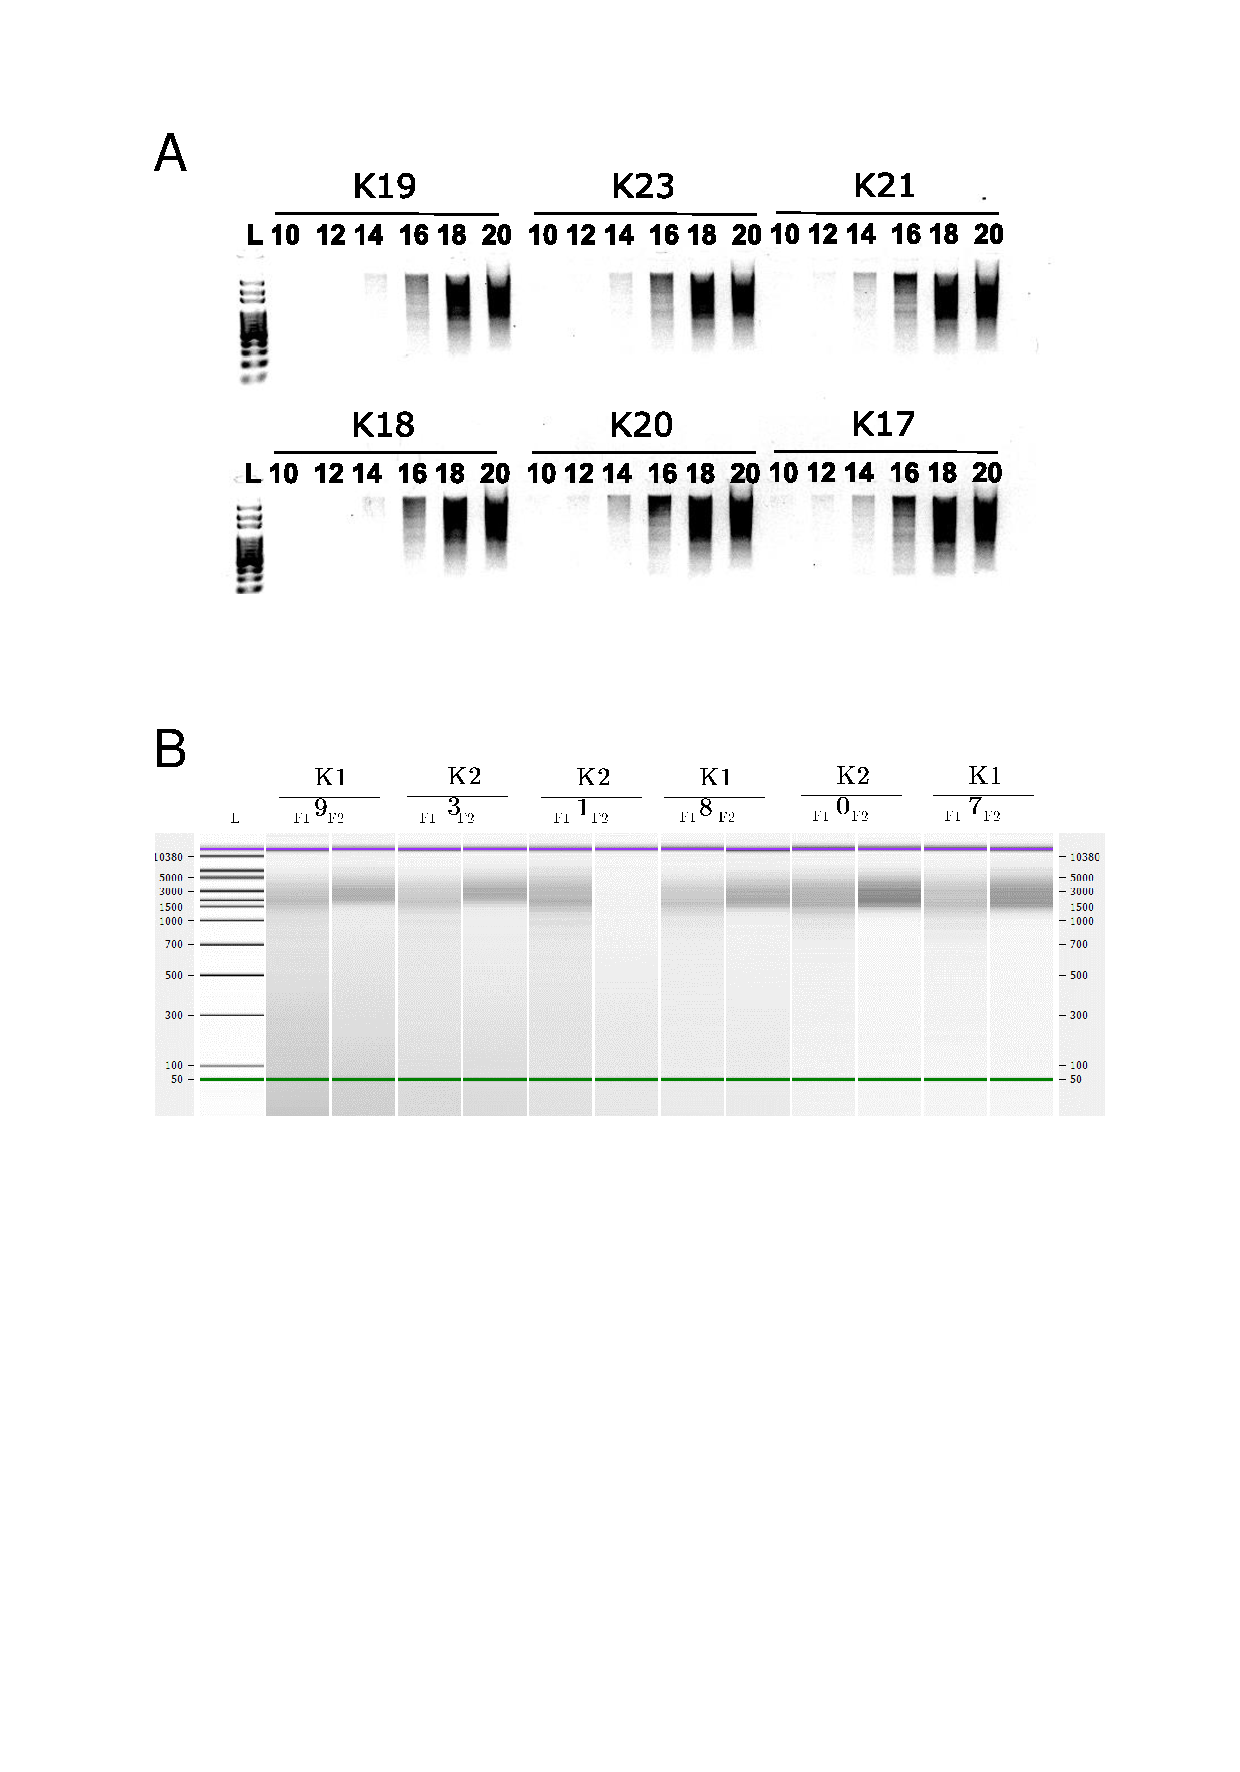
\includegraphics[page=1,trim={0 10cm 0 0cm},clip,scale = 0.75]{Figures/TargetedTranscriptome_LabResults.pdf}
	\captionsetup{width=0.95\textwidth}
	\caption[Iso-Seq targeted profiling - PCR cycle optimisation]%
	{\textbf{Samples for targeted profiling were amplified with 14 PCR cycles.} Shown is \textbf{(A)} an example of an agarose gel image from PCR cycle optimisation of six mouse samples after cDNA synthesis. Analogous to global transcriptome profiling (\cref{fig:isoseq_whole_pccresults}), 14 cycles were determined to be optimal for large scale amplifications. Ladder (L) denotes to a 100bp DNA ladder. \textbf{(B)} A Bioanalyzer gel of amplified cDNA after purification with 1X (F1) and 0.4X (F2) AMPure beads. Size distribution for each fraction was determined from the start to the end point of the smear. Ladder (L) denotes to a 12kb DNA ladder, whereby the green and purple line represent the lower marker at 50bp and the upper marker at 12kb, respectively.}
	\label{fig:isoseq_targeted_pccresults}
\end{figure}


\begin{figure}[!htp]
	\centering
	\vspace{20pt}
	\includegraphics[page=2,trim={0 15cm 0cm 1cm},clip,scale = 0.75]{Figures/TargetedTranscriptome_LabResults.pdf}
	\captionsetup{width=0.95\textwidth}
	\caption[Iso-Seq targeted profiling - target capture \& SMRTbell library preparation]%
	{\textbf{Successful target capture and Iso-Seq library preparation.} Shown are Bioanalyzer electropherograms of \textbf{(A)} batch 1 (n = 6 samples) after target enrichment and \textbf{(B)} Iso-Seq library preparation, and \textbf{(C)} batch 2 (n = 9 samples) after target enrichment and \textbf{(D)} Iso-Seq library preparation. 
	\\
	\\
	Illustrating successful target enrichment, we observed peaks that correspond to enriched transcript lengths from genes of interest, which notably differs from the broad peaks seen in Iso-Seq global dataset (\cref{fig:isoseq_whole_bioresults}). Iso-Seq library preparation retained these target transcripts with detection of similar peaks, albeit less pronounced due to a lower cDNA input for Bioanalyzer assays in order to conserve cDNA for maximum sequencing yield.}  
	\label{fig:isoseq_targeted_libresults}
\end{figure}

\begin{figure}[!htp]
	\centering
	\vspace{20pt}
	\includegraphics[page=3,trim={0 17cm 0cm 0cm},clip,scale = 0.75]{Figures/TargetedTranscriptome_ppt.pdf}
	\captionsetup{width=0.95\textwidth}
	\caption[ONT targeted profiling - target capture \& library preparation]%
	{\textbf{Successful target capture and ONT library preparation.} Shown in \textbf{(A)} is the TapeStation gel of batch 2 (n = 9) and batch 3 (n = 9) after target enrichment and ONT library preparation, and \textbf{B)} is the respective TapeStation electropherogram of batch 3. 
	\\
	\\
	Illustrating successful target enrichment analogous to \cref{fig:isoseq_targeted_libresults}, we observed peaks that correspond to enriched transcript lengths from genes of interest. Lower cDNA input was used for TapeStation assays to maximise the amount of cDNA available for sequencing. L - Ladder, B2 - batch 2, B3 - batch 3.}  
	\label{fig:ONT_targeted_libresults}
\end{figure}

\newpage
\subsection{SMRT sequencing QC and data processing}
The processing of raw reads was performed using the Iso-Seq bioinformatics pipeline (outlined in \cref{section:isoseq_bioinformatics}), in an approach analogous to that used in the processing of the Iso-Seq global dataset with the exception of sample demultiplexing using barcode-specific sequences. Briefly, CCS reads were generated from a minimum of 1 pass (\textit{Iso-Seq3 CCS}, v3.4.1) for each batch followed by removal of primers and barcode sequences using \textit{Lima} (v1.9) to generate full-length (FL) reads for each sample. After removal of artificial concatemer reads and trimming of polyA tails using \textit{Iso-Seq3 Refine}, full-length reads were then merged and collapsed to high quality transcripts using \textit{Cupcake} (parameters: -c 0.85 -i 0.95 --dun-merge-5-shorter), and mapped to the mouse reference genome (mm10) using \textit{Minimap2} (v2.17). Full-length Iso-Seq read counts from each individual sample were extracted from \textit{Cupcake's} read\_stat.txt file using the CCS read ID as sample identifier.

\subsection{ONT nanopore sequencing QC and data processing}
The QC of raw reads was performed using PycoQC followed by subsequent analysis using the ONT bioinformatics pipeline (details are provided in \cref{section:ont_bioinformatics}). Briefly, raw reads were basecalled using \textit{Guppy} (v4.0) and reads with Phred (Q) < 7 were filtered. Primers and ONT adapters were then removed using \textit{Porechop} (v0.2.4) to generate full-length reads for each sample. After trimming of polyA tails using \textit{Cutadapt} (v2.9), full-length reads were then mapped to the reference mouse genome (mm10) using \textit{Minimap2} (v2.17, parameters: "-ax splice"). Owing to the high error rate of ONT nanopore sequencing, artefactual non-canonical splice junctions from mapped reads were corrected with \textit{Transcript Clean}. Corrected reads were then processed using \textit{TALON} (v5.0) for annotation, quantification and filtering for intrapriming (--maxFracA = 0.5). Novel transcripts were only retained if they were covered by >5 full-length reads and detected in >2 samples. \textit{TALON} was chosen as the preferred tool for ONT processing after trialling multiple tools (more details are provided in \textbf{Appendix} \textbf{\ref{ONT_Bioinformatics_appendix}}). 

\subsection{Comparison of Iso-Seq and ONT datasets}
The Iso-Seq targeted dataset (n = 24 samples) was examined with other datasets using \textit{Gffcompare}; such datasets included Iso-Seq-derived transcripts identified from global transcriptome profiling (n = 12 samples, \cref{tab:isoseq_wholerun_result}, Iso-Seq global dataset) and ONT-derived transcripts from targeted profiling (n = 18 samples, \cref{tab:mouse_samples_sequenced}, ONT targeted dataset). For a fair comparison, the Iso-Seq global dataset was re-annotated with \textit{SQANTI3} with no splice junction filtering from short-read RNA-Seq data, and only transcripts derived from matched samples were used for comparison. Conversely, all processed but unfiltered ONT reads were used for a comprehensive comparison between the two technologies with Iso-Seq derived transcripts as reference. 

\begin{figure}[htp]
	\centering
	\includegraphics[page=16,trim={0cm 8cm 0cm 0cm},clip,scale = 0.8]{Figures/ProjectDevelopment_Figures}
	\captionsetup{width=0.95\textwidth,singlelinecheck=off}
	\caption[Detailed ONT bioinformatics pipeline for targeted profiling]%
	{\textbf{Detailed ONT bioinformatics pipeline for targeted profiling.} Shown is a detailed bioinformatics pipeline for processing ONT reads from targeted profiling after sequencing of the rTg4510 cortex (S\textsubscript{n}) on two flow cells (referred as batch 2 and batch 3 of the Iso-Seq targeted dataset, summarised in \cref{tab:mouse_samples_sequenced}). Supplementing \cref{fig:ONT_PacBio_bioinformatics}, raw ONT reads from each flow cell were processed and demupliplexed using \textit{Porechop} to generate sample-specifici reads, which were subsequently processed independently for collapse and transcript quantification. Samples from both batches were then merged into one dataset, while retaining sample-specific transcript expression. 
	}
	\label{fig:ONT_Targeted_bioinformatics}
\end{figure}

\subsection{Merged annotation and quantification}
\label{ch6: methods_quantification}
For a comprehensive characterisation of the target genes enriched in the rTg4510 cortex, full-length transcripts from the Iso-Seq and ONT targeted datasets were merged using \textit{Gffcompare} (depicted in \cref{fig:Targeted_bioinformatics_pipeline}). A custom python script ("identify\_common\_targeted\_transcripts.py") was then applied to: i) identify transcripts detected using both PacBio Iso-Seq and ONT nanopore sequencing, which were defined as a complete exact match in \textit{Gffcompare} output (class code: "="), ii) retain ONT-derived novel transcripts that did not pass \textit{TALON} filtering (>5 reads and detected in >2 samples), but were detected in the Iso-Seq targeted dataset, iii) retain all transcripts unique to the Iso-Seq targeted dataset given the stringent processing and high accuracy of Iso-Seq reads, and iv) generate an abundance file for each sample and transcript, either tabulating counts from \textit{Cupcake} for Iso-Seq-derived-transcripts, counts from \textit{TALON} for ONT-derived-transcripts or the count summation for commonly detected transcripts. The merged dataset was then annotated with \textit{SQANTI3} in combination with mouse reference gene annotations (mouse GENCODE, vm22), FANTOM5 CAGE peaks and \textit{STAR}-aligned RNA-Seq junctions. Isoform were subsequently classified as either FSM, ISM, NIC, NNC, antisense, fusion, and intergenic (described in \cref{section: sqanti_annotations}). Isoforms classified as ISM with 3'fragment were assumed to be partial 5'RNA degraded products and removed. 

\begin{figure}[htp]
	\centering
	\includegraphics[page=5,trim={0.5cm 7cm 0cm 0cm},clip,scale = 0.8]{Figures/TargetedTranscriptome_LabResults}
	\captionsetup{width=0.95\textwidth,singlelinecheck=off}
	\caption[Bioinformatics pipeline for merging targeted Iso-Seq and ONT datasets]%
	{\textbf{Bioinformatics pipeline for merging targeted Iso-Seq and ONT datasets.} Shown is a outline of the bioinformatics pipeline for processing Iso-Seq reads and ONT reads 1D reads from the targeted profiling of the mouse cortex. 
	}
	\label{fig:Targeted_bioinformatics_pipeline}
\end{figure}

\subsection{Quantification of human MAPT transgene expression} 
The presence of human- and mouse-specific \textit{Mapt/MAPT} sequences was determined in full-length transcripts as QC check of sample identity (as detailed in \cref{ch5: hmapt_quant}). 

\newpage
\subsection{Characterisation of AS events and transcript visualisation}
\label{ch6: methods_characterisation}
Existing tools for assessing alternative splicing events were developed for analysing short-read RNA-Seq data and fail to capture the connectivity and complexity of long-read-derived isoforms, particularly in targeted profiling where deep sequencing coverage is achieved. A custom python script ("annotate\_common\_targeted\_transcripts.py") was therefore developed to accurately assess the occurrence of alternative splicing events by comparing splice sites (exon) coordinates between long-read-derived transcripts and reference transcripts (mm10) (depicted in \cref{fig:Targeted_bioinformatics_pipeline}). Common alternative splicing events such as alternative first exons (AF), alternative last exons (AL), alternative 5' splice sites (A5), alternative 3' splice sites (A3), intron retention (IR) and exon skipping (ES) were assessed (depicted in \cref{fig:AS_events}). Alternative 5' and 3' splice sites were defined as splice sites differing by more than 10bp from the known splice site, and an intron was considered retained if the exon splice site differed by more than 100bp from the known splice site (depicted in \cref{fig:Targeted_isoforms_annotate}). Other regulatory mechanisms such as alternative transcription initiation (defined by alternative TSS) and termination (defined by alternative TSS), and the presence of novel exons, were also evaluated. 

Open reading frames were predicted using the Coding-Potential Assessment Tool\cite{Wang2013b} (CPAT) (v3.0.2) under default parameters, and transcripts with coding potential score >0.44 (recommended threshold) were predicted as protein-coding. Isoforms were predicted as being characterised by nonsense-mediated decay if the distance between predicted open read frame and last exon-exon junction was >50bp. Finally, a separate custom python script ("colour\_common\_targeted\_transcripts.py") was applied to colour transcripts by coding potential (green for protein coding, red for non-protein coding) and also shade them by abundance. Isoforms were then grouped by splicing patterns and visualised using the UCSC genome browser. 

\begin{figure}[htp]
	\centering
	\includegraphics[page=7,trim={0cm 3cm 0cm 0cm},clip,scale = 0.75]{Figures/TargetedTranscriptome_LabResults}
	\captionsetup{width=0.95\textwidth,singlelinecheck=off}
	\caption[Characterisation of isoforms detected in targeted profiling]%
	{\textbf{Characterisation of isoforms detected in targeted profiling.} \textbf{(A)} Reference transcripts were "flattened" to obtain splice site coordinates. \textbf{(B)} Exon-level comparison of long-read-derived transcripts and reference transcripts was then performed by comparing splice site coordinates to assess occurrence of alternative splicing sites. Splice sites differing <10bp ("wobble") were considered identical, >10bp as truncation, >10bp but <100bp as extension ,and >100bp as intron retention.  
	}
	\label{fig:Targeted_isoforms_annotate}
\end{figure}

\begin{figure}[htp]
	\centering
	\includegraphics[page=8,trim={0cm 1cm 0cm 0cm},clip,scale = 0.75]{Figures/TargetedTranscriptome_LabResults}
	\captionsetup{width=0.95\textwidth,singlelinecheck=off}
	\caption[Visualising isoforms by coding potential, abundance and NMD status]%
	{\textbf{Visualising isoforms by coding potential, abundance and NMD status.} Shown is a flow-diagram for isoform visualisation. \textbf{(A)} Open reading frames were determined using \textit{CPAT} and \textbf{(B)} isoforms were subsequently coloured by protein coding potential (green for coding, red for non-coding, and gray for no open reading frame) and shaded by abundance (described in \cref{ch6: methods_quantification}). \textbf{(C)} A schematic figure illustrating approach for predicting nonsense-mediated decay (NMD). ORF - Open Reading Frame. 
	}
	\label{fig:Targeted_isoforms_cpat}
\end{figure}

\newpage
\subsection{Differential analysis}
Differential expression analysis was performed with \textit{tappAS} using full-length read counts from Iso-Seq and nanopore sequencing (fully described in \cref{ch3_tappas_explained}). Briefly, \textit{tappAS} filters out lowly-expressed isoforms, normalises read counts using TMM approach and performs differential expression analysis using \textit{maSigPro}\cite{Conesa2006,Nueda2014,Conesa2017} to elucidate effects for both genotype and age. Normalised counts generated from \textit{tappAS} were used to generate plots illustrating differential expression changes. Gene expression was deduced from the summation of normalised counts from associated isoforms. Plots showing the distribution of isoform expression (i.e. isoform usage) were determined by dividing the mean of each isoform across biological replicates (n = 3) over the total mean expression of all the isoforms. Minor isoforms with low expression (mean expression < 0.5 counts in WT and TG) were removed, and isoforms that make up < 5\% were classified under "Other". 

\newpage
\section{Results}
\subsection{Iso-Seq run performance and sequencing metrics}
Following Iso-Seq library preparation and SMRT sequencing, we generated a total of 62.8Gb sequencing data (n = 24 samples, mean yield = 20.9Gb, s.d = 2.84Gb, range = 19.25Gb - 24.2Gb, \cref{tab:targeted_mouse_run_output}). While the sequencing yield was comparable to global transcriptome profiling (\cref{tab:isoseq_wholerun_result}), the run performance varied across the three Iso-Seq targeted datasets, particularly between batch 1 (n = 6 samples) and batches 2 (n = 9 samples), 3 (n = 9 samples), which were sequenced pre- and post-Covid-19 lockdown respectively. The run performance metrics for batch 1 were optimal (\cref{tab:targeted_mouse_run_output}). Conversely, batches 2 and 3 had a poor loading rate (batch 1 P1:  71\%, batch 3 P1: 38.1\%) with sequencing yields that were comparable to batch 1, despite containing more samples. We suspect that this reduced run performance was likely a result of relative sample degradation, given samples were stored in -20\textdegree C for >9 months (due to Covid-19 lockdown) before sequencing. 

Following the Iso-Seq bioinformatics pipeline, raw reads were processed and clustered to unique consensus transcripts, which were then mapped to the mouse reference genome. A total of 966K CCS reads (mean = 332K, s.d = 126K, range =  221K - 469K) and 930K FLNC reads (mean = 310K, s.d = 77.7K, range = 2556K - 399K) were successfully generated (\cref{fig:isoseq_targeted_run_output}\textbf{A}). Where there was evident difference in the number of CCS reads obtained for batch 1 and batches 2,3 - a reflection of the run performance - batches 2 and 3 had a significantly greater coverage of target genes than batch 1 (\cref{fig:isoseq_targeted_rate}). These results indicate that the sub-optimal run performance and subsequent lower sequencing yield of batches 2 and 3 were compensated by a bigger sample size, generating more full-length reads associated to target genes. In contrast, the better run performance but lower sample size of batch 1 resulted in quicker saturation of target genes and the generation of more full-length reads associated to off-target genes. 

Finally, we noted that the number of full-length transcripts obtained per sample varied within each batch (\cref{fig:isoseq_targeted_run_output}\textbf{B}), despite the careful pooling of samples with equal molarity during library preparation. This variability was not associated with RIN (corr = 0.147, P = 0.492, Spearman's rank). However, no significant difference in the number of full-length transcripts was observed between WT and TG across the runs (Wilcoxon rank sum test, W = 73, P = 0.977, \cref{fig:isoseq_targeted_run_output}\textbf{C}). 


\begin{table}[]
	\captionsetup{width=1.0\textwidth}
	\caption[Iso-Seq sequencing yield for targeted profiling of rTg4510 mouse cortex]%
	{\textbf{Iso-Seq sequencing yield for targeted profiling of the rTg4510 mouse cortex.} rTg4510 cortex (n = 9 WT, n = 9 TG) was sequenced using the Iso-Seq approach on 3 runs (batch 1, 2 and 3) after multiplexing and enrichment of 20 AD-associated genes. Further details on evaluation of the performance of Iso-Seq sequencing runs are provided in \cref{sec: Isoseq_run_performance}. K - Thousand, Pol - Polymerase. N50 is defined as the sequence length of the shortest read at 50\% of all reads}
	\label{tab:targeted_mouse_run_output}
	\centering
	\setlength\tabcolsep{6pt} %reduced margin size in table
	\begin{tabularx}{\textwidth}{cccccccccc}
		\toprule
		\multirow{3}{*}{Runs} &
		\multirow{3}{*}{\begin{tabular}[c]{@{}c@{}}Total \\ Bases\\ (Gb)\end{tabular}} &
		\multirow{3}{*}{\begin{tabular}[c]{@{}c@{}}Polymerase\\  Reads (K)\end{tabular}} &
		\multicolumn{4}{c}{Read Length (kB)} &
		\multicolumn{3}{c}{Productivity} \\ \cmidrule(l){4-10} 
		&&&
		\multicolumn{2}{c}{Polymerase} &
		\multicolumn{2}{c}{Subread} &
		\multirow{2}{*}{P0} &
		\multirow{2}{*}{P1} &
		\multirow{2}{*}{P2} \\
		&&&
		Mean & N50 & Mean & N50 &&&
		\\ \midrule
		batch 1 & 24.2 & 712 & 34.0 & 70.5 &	1.4 & 1.85 &
		\begin{tabular}[c]{@{}c@{}}4.62\% \\ (46613)\end{tabular} &
		\begin{tabular}[c]{@{}c@{}}71.58\% \\ (722026)\end{tabular} &
		\begin{tabular}[c]{@{}c@{}}24.76\% \\ (249707)\end{tabular} \\
		batch 2 &
		&&&&&&&
		&
		\\
		batch 3 &	19.3 &	384 &	50.5 &	100 &	1.6 &
		2.02 &
		\begin{tabular}[c]{@{}c@{}}18.68\% \\ (189549)\end{tabular} &
		\begin{tabular}[c]{@{}c@{}}38.11\% \\ (386743)\end{tabular} &
		\begin{tabular}[c]{@{}c@{}}43.56\% \\ (442054)\end{tabular} \\ \bottomrule
	\end{tabularx}
\end{table}


\begin{figure}[!htp]
	\begin{center}
		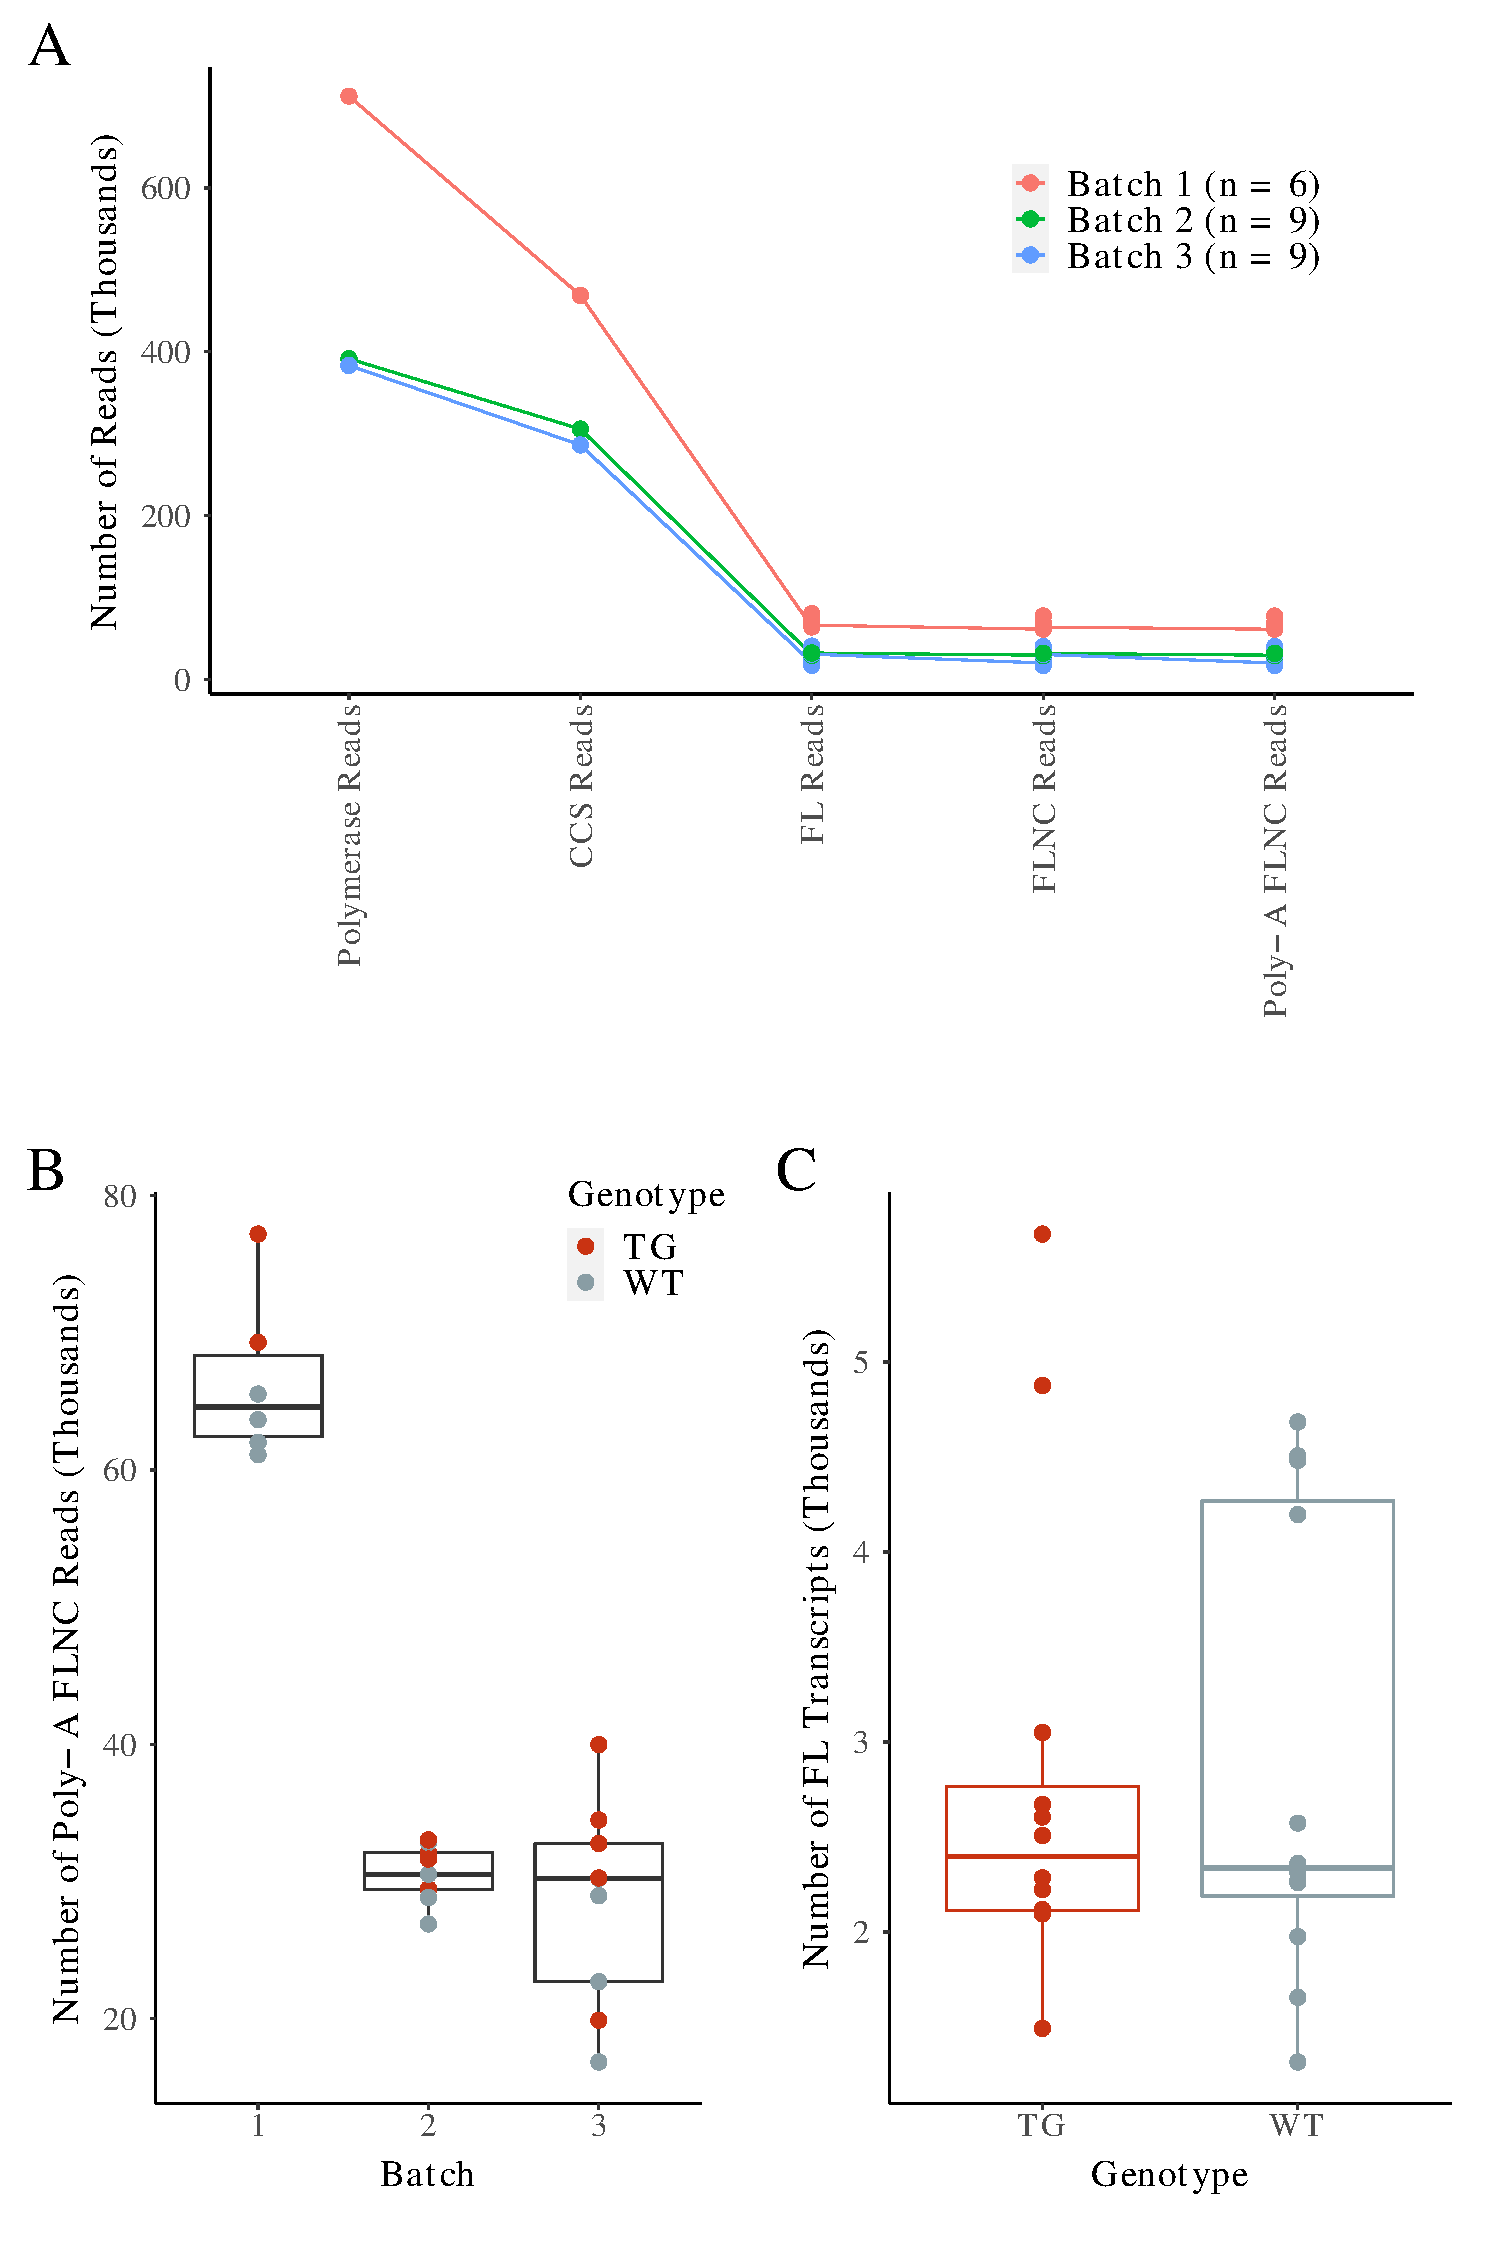
\includegraphics[page=1,trim={0 1cm 0 0},clip,scale = 0.55]{Figures/TargetedTranscriptome.pdf}
	\end{center}
	\captionsetup{width=0.95\textwidth}
	\caption[Iso-Seq sequencing metrics from targeted profiling of rTg4510 mice]%
	{\textbf{Despite batch variability in Iso-Seq targeted datasets, no difference was reported in the number of FL transcripts between WT and TG mice.} Shown is \textbf{(A)} a scatter plot of the number of reads generated through the Iso-Seq bioinformatics pipeline from initial generation of CCS reads, to FL reads with primer removal, and poly-A FLNC reads with removal of artificial concatemers and trimming of poly(A) tails. Samples were multiplexed and sequenced in three runs (batch 1, 2 and 3). Shown are box-plots of the \textbf{(B)} number of poly-A FLNC reads by batch and genotype and \textbf{(C)} final number of FL transcripts by genotype. CCS - Circular Consensus Sequence, FLNC - Full-Length Non-Concatemer, FL - Full-Length, WT - Wild-type mice, TG - rTg4510 transgenic mice}
	\label{fig:isoseq_targeted_run_output}
\end{figure}

\begin{figure}[!htp]
	\centering
		\includegraphics[page=2,trim={0 25cm 0 0},clip,scale = 0.55]{Figures/TargetedTranscriptome.pdf}
	\captionsetup{width=0.95\textwidth}
	\caption[On-target rate of Iso-Seq targeted profiling]%
	{\textbf{Higher coverage of target genes in batches 2 and 3 due to more samples multiplexed and sequenced.} Shown is a box-plot of the on-target rate, defined as the proportion of mapped transcripts associated with target genes (AD-associated genes) with overlapping sequences to at least one target probe. Of note, a difference in the on-target rate between WT and TG in batch 1 is a likely reflection of the sample variability in sequencing (\cref{fig:isoseq_targeted_run_output}\textbf{B}). WT - Wild-type, TG - rTg4510 transgenic mice.}
	\label{fig:isoseq_targeted_rate}
\end{figure}

\newpage
\subsection{Iso-Seq targeted profiling approach detects many novel, rare isoforms annotated to AD-associated genes}
\label{ch6: wholevstargeted}
Following stringent quality-control and filtering of technical artefacts, we detected 19,659 isoforms in the Iso-Seq targeted dataset of which 2,015 isoforms (10.2\%) were annotated to 20 AD-associated genes enriched in the rTg4510 cortex (n = 12 WT, n = 12 TG). This was in stark contrast to the global transcriptome profiling dataset, where we detected 175 isoforms (0.25\% of total number of isoforms detected from global transcriptome profiling) annotated to the same AD-associated genes, highlighting the power of targeted profiling for deep coverage of target genes. As expected, target enrichment and sequencing of matched samples (n = 6 WT, 6 TG, \cref{tab:whole_phenotype}) detected many more AD-associated transcripts than the whole transcriptome profiling approach (\cref{fig:targeted_vs_whole}\textbf{A}, Iso-Seq global dataset: n = 46 unique isoforms, Iso-Seq targeted dataset = 658 unique isoforms, Iso-Seq global and targeted dataset = 221 isoforms). The majority of these isoforms unique to the Iso-Seq targeted dataset were novel (\cref{fig:targeted_vs_whole}\textbf{B}, n = 525 isoforms, 79.8\%) as NIC (n = 218 isoforms, 33.1\%) and NNC (n = 307 isoforms, 46.7\%), and less abundant (\cref{fig:targeted_vs_whole}\textbf{D}), highlighting the greater sensitivity of the targeted profiling approach to detect the novel, rarer transcripts. Strikingly, the global transcriptome profiling approach detected all the target genes with the exception of \textit{Trpa1}, the most lowly-expressed target gene in the mouse cortex (\cref{tab:target_genes_description}), which suggests that the gene sensitivity with 5.6 million CCS reads (n = 12 samples) using the Iso-Seq global transcriptome profiling approach was capped between 0.1 TPM (mouse cortex \textit{Trpa1} expression) and 0.5 TPM (mouse cortex \textit{Rhbdf2} expression, the second least expressed target gene). Given that our Iso-Seq global datasets approached saturation particularly at the gene level (\cref{fig:isoseq_whole_rarefaction}\textbf{A}), it is unlikely that we would have been able to detect \textit{Trpa1} transcripts with more samples using the global transcriptome profiling approach.

Further comparison of the isoform landscape of AD-associated genes in the Iso-Seq global and targeted datasets revealed a similar distribution of isoform length (Iso-Seq global dataset: mean = 2.67kb, s.d = 1.6kb, range = 300bp - 10.3kb, Iso-Seq targeted dataset: mean = 2.4kb, s.d = 1.2kb, range = 140bp - 10.3kb; Mann-Whitney-Wilcoxon test: W = 1.91 x 10\textsuperscript{6}, P = 0.068) and number of exons (Iso-Seq global dataset: mean = 12.9, s.d = 9.6, range - 1 - 50; Iso-Seq targeted dataset: mean = 11.7, s.d = 7.9, range = 1 - 50; Mann-Whitney-Wilcoxon test: W = 1.86 x 10\textsuperscript{6}, P = 0.22). Drawing parallels to the isoform landscape of the global transcriptome, approximately half of the isoforms identified in Iso-Seq targeted dataset were novel (n = 919 isoforms, 45.6\%) as NIC (n = 485, 24.1\%) and NNC (n = 434 isoforms, 21.5\%) (\cref{fig:isoseq_targeted_finalnumberiso}\textbf{A}), with the remaining half identified as known and predominantly ISM (n = 913, 45.3\%). However, AD-associated isoforms in Iso-Seq targeted dataset were less enriched near CAGE peaks from the FANTOM5 dataset (median distance from CAGE peak = 335 bp, 646 transcripts located within 50bp of a CAGE peak) than AD-associated isoforms detected in Iso-Seq global dataset (median distance from CAGE peak = 2 bp, 122 transcripts (69.7\%) located with 50bp of a CAGE peak), and were located further to annotated transcription start sites (Iso-Seq targeted dataset: median distance = 808bp, Iso-Seq global dataset: median distance = 8bp) and transcription termination sites (Iso-Seq targeted dataset: median distance = 2bp, Iso-Seq global dataset: median distance = 1bp). 

Generating highly parallel RNA-Seq data on the same samples (n = 24 samples, total number of uniquely mapped reads = 360 million), we further found that the vast majority of these isoforms were not supported by RNA-Seq reads spanning the junction (n = 1658 isoforms, 82.2\%). Given the stringent process of the Iso-Seq bioinformatics pipeline and target enrichment, this likely reflects the low coverage of RNA-Seq reads to comprehensively span these novel junctions and the elevated power of long-read sequencing to detect profile transcript structure. However, a strong correlation between gene-level expression level was observed across both methods (n = 20 genes, corr = 0.86, P = 1.18 x 10\textsuperscript{-6}), \cref{fig:isoseq_targeted_finalnumberiso}\textbf{B}). 

Finally, we observed a relatively high off-target rate of Iso-Seq targeted experiments with detection of isoforms (n = 17,644, 89.8\%) that were not associated with target genes. Comparison with the Iso-Seq global datasets using matched samples (n = 12, n = 7,925 off-target isoforms, 89.8\%) revealed that the overwhelming majority of these isoforms (n = 7,418, 93.6\% off-target isoforms) were also detected in the Iso-Seq global dataset. These isoforms were more abundant than isoforms unique to the Iso-Seq global dataset and isoforms associated to target genes (\cref{fig:targeted_vs_whole}\textbf{C}), suggesting that capture of off-target genes is predominantly driven by abundance rather than sequence homology to target genes (off-target binding).  

\begin{figure}[!htp]
	\centering
	\includegraphics[page=3,trim={0 1.5cm 0 0cm},clip,scale = 0.50]{Figures/TargetedTranscriptome.pdf}
	\label{fig:targeted_vs_whole}
	\captionsetup{width=0.95\textwidth}
	\caption[Comparison of Iso-Seq global transcriptome and targeted profiling]%
	{\textbf{Iso-Seq targeted approach detected many more novel and rarer transcripts than global transcriptome profiling of the mouse cortex.} Shown are \textbf{(A)} bar-plots of the number of isoforms per target gene that were uniquely detected using the Iso-Seq targeted profiling approach ("Targeted"), uniquely detected in the Iso-Seq global transcriptome profiling approach ("Whole") and in both datasets ("Both"), and the \textbf{(B)} bar-plots of the number of isoforms in the Iso-Seq targeted approach stratified by structural category. \textbf{(C)} A box-plot of the full-length read counts of isoforms associated to target and non-target genes in the Iso-Seq global and \textbf{(D)} targeted datasets. Target genes refer to the panel of 20 AD-associated genes that were enriched for targeted sequencing. Only transcripts from matched samples were compared. FSM - Full Splice Match, ISM - Incomplete Splice Match, NIC - Novel In Catalogue, NNC - Novel Not in Catalogue.}
\end{figure}

\begin{figure}[!htp]
	\begin{center}
		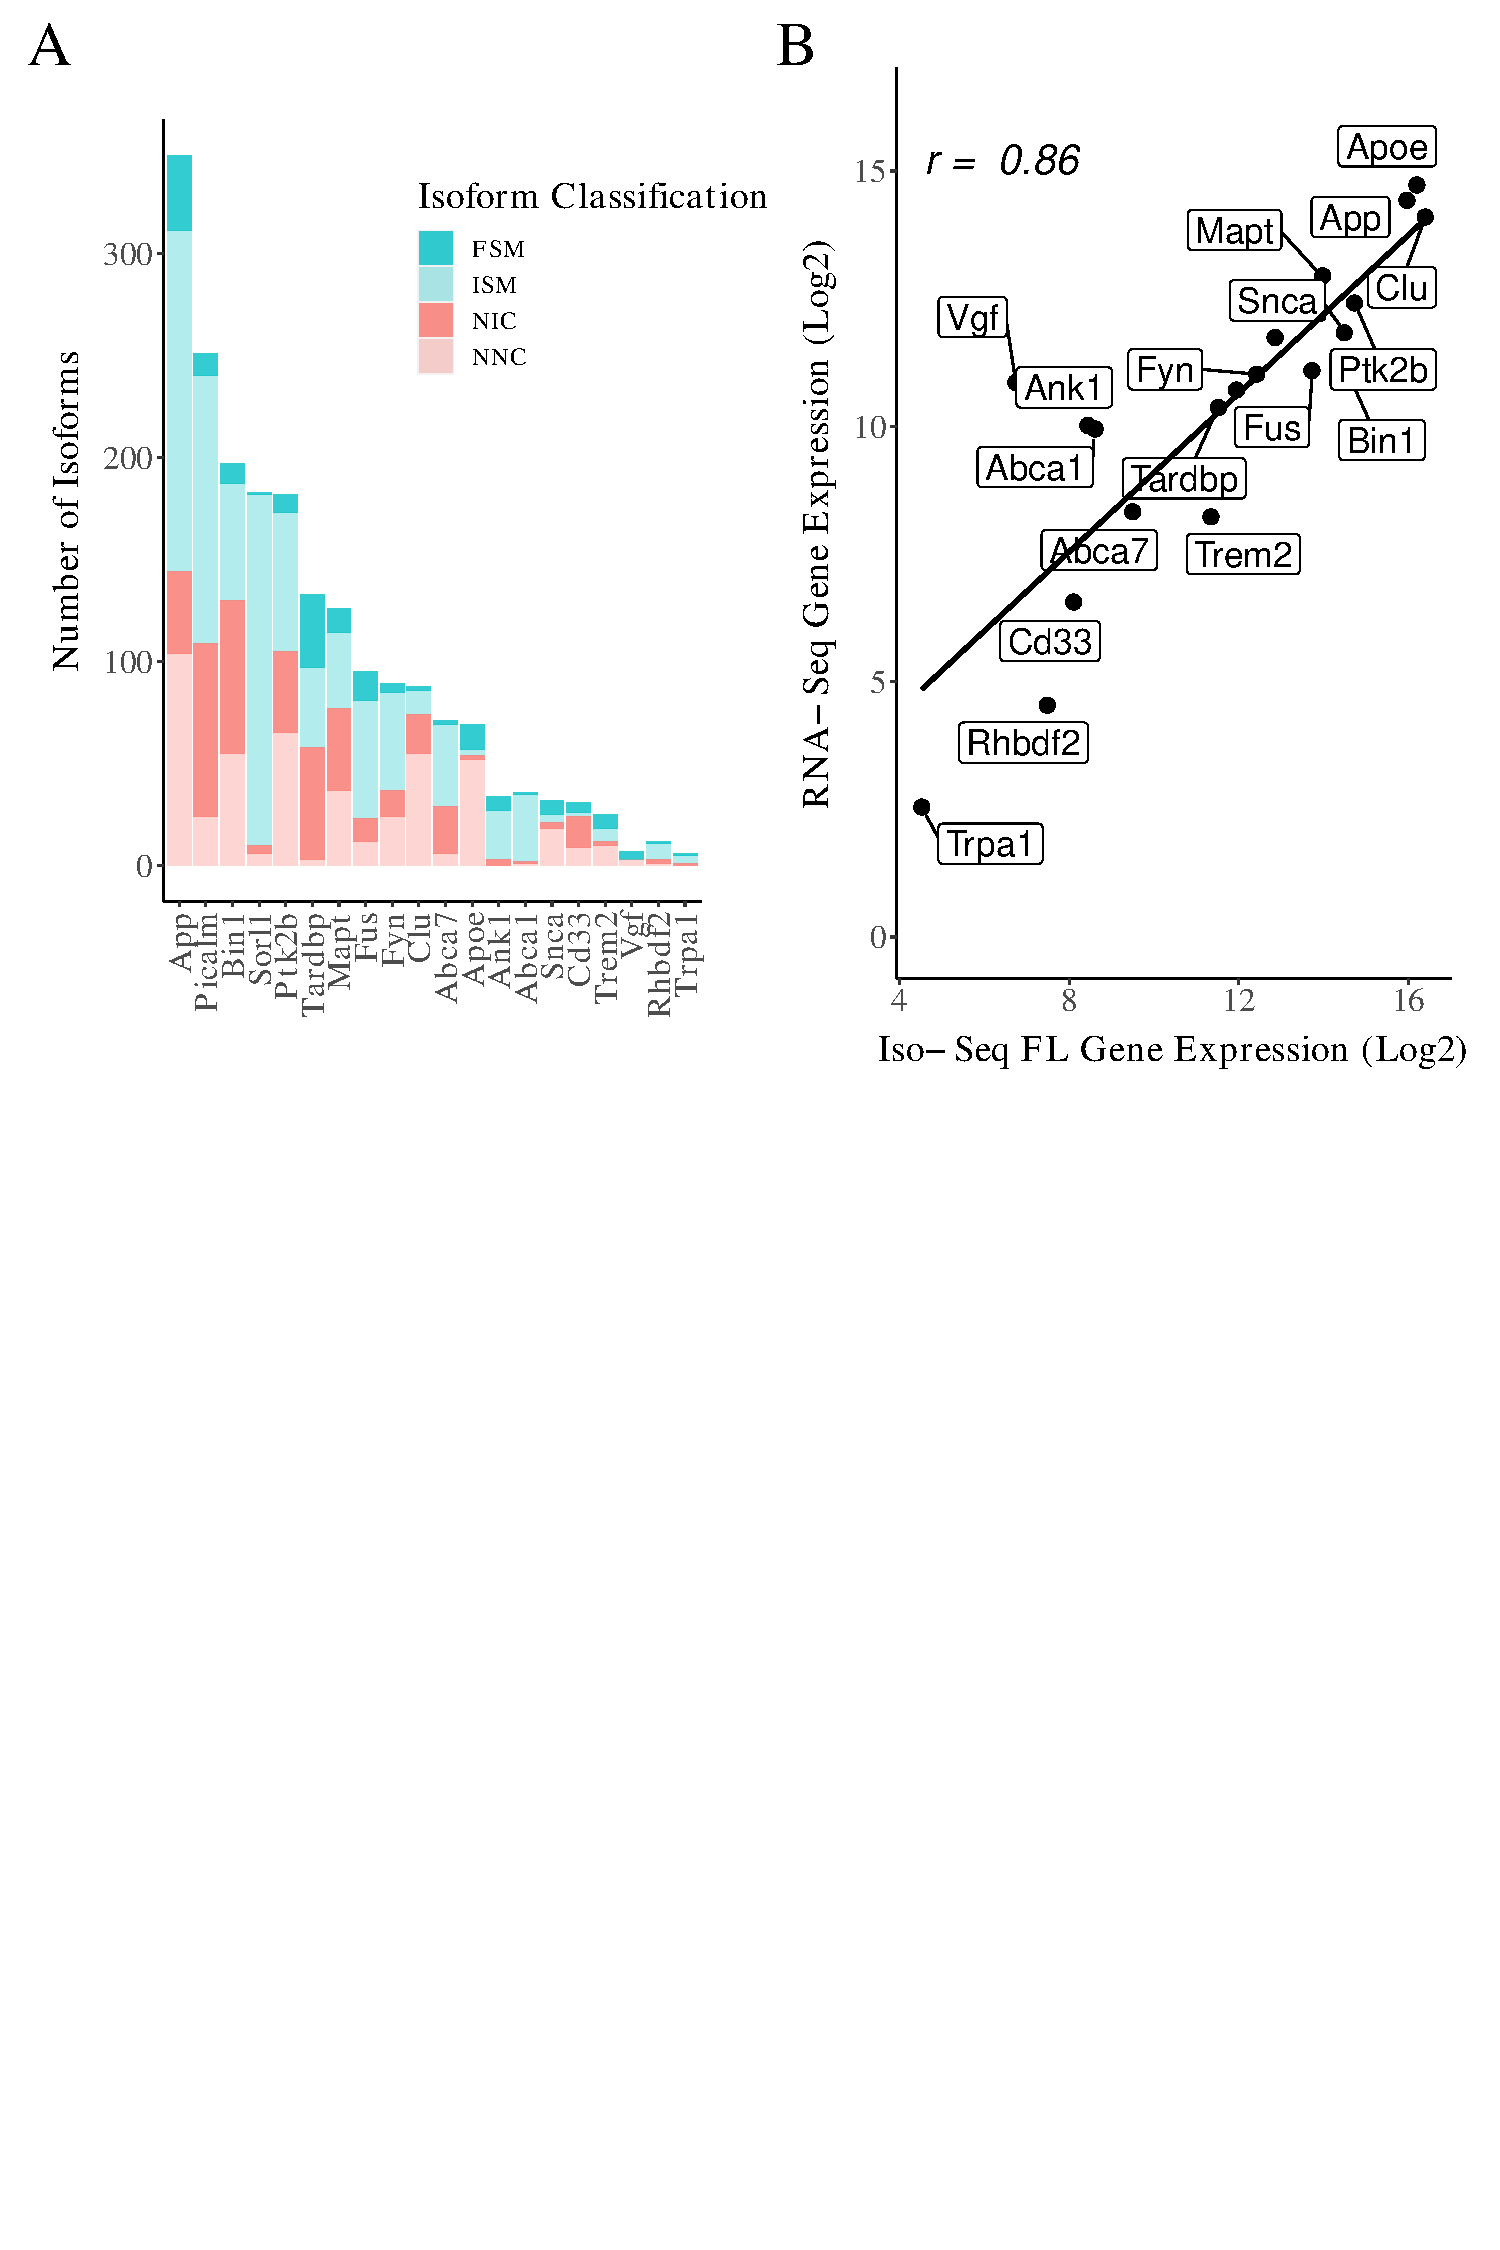
\includegraphics[page=1,trim={0 20cm 0 0cm},clip,scale = 0.60]{Figures/ONTvsIsoSeq.pdf}
	\end{center}
	\captionsetup{width=0.95\textwidth}
	\caption[Isoform landscape of AD-risk genes from Iso-Seq targeted profiling]%
	{\textbf{Widespread isoform diversity was observed in AD-risk genes with detection of many novel isoforms in the rTg4510 cortex.} Shown is \textbf{(A)} a bar plot of the number of isoforms detected per AD-risk gene from the Iso-Seq targeted dataset, classified by novel and known, after sequential processing and filtering in the bioinformatics Iso-Seq pipeline, and \textbf{(B)} a density plot of the RNA-Seq and Iso-Seq gene expression. Iso-Seq gene expression was determined from the summation of full-length read counts of associated transcripts, whereas RNA-Seq gene expression was deduced from the normalised \textit{DESeq} counts of aligned RNA-Seq reads to reference genome\cite{Castanho2020}.}
	\label{fig:isoseq_targeted_finalnumberiso}
\end{figure}

\newpage
\subsection{Confirmation that the \textit{MAPT} transgene is only expressed in rTg4510 TG mice}
The mouse \textit{Mapt} gene was one of the 20 target genes enriched for the targeted profiling of the rTg4510 mouse cortex. Given the high homology between the mouse \textit{Mapt} and human \textit{MAPT} coding sequence (as seen in \cref{mapt_transgene_whole} ), we anticipated that the target enrichment approach would also capture the human \textit{MAPT} transgene. As expected, BLAST analysis of the species-specific \textit{Mapt/MAPT} sequences showed only detection of the human-specific \textit{MAPT} sequences in reads from TG mice (\cref{fig:hmapt_ont_isoseq}\textbf{A,B}), confirming stable activation of the human \textit{MAPT} transgene. There was also an enrichment of full-length reads corresponding to the mouse \textit{Mapt} gene, which was not previously noticeable in the Iso-Seq global dataset (\cref{fig:isoseq_humanmapt}\textbf{A}), as a further testament to the success of the targeted experiments. Notably, there was a striking difference in the number of reads corresponding to the human \textit{MAPT} transgene and the mouse \textit{Mapt} gene in the ONT targeted dataset (\cref{fig:hmapt_ont_isoseq}\textbf{B}) - a likely reflection of the extra-deep sequencing coverage provided using ONT nanopore sequencing. 

\begin{figure}[!htp]
	\begin{center}
		\includegraphics[page=12,trim={0 20cm 0 0cm},clip,scale = 0.60]{Figures/ONTvsIsoSeq.pdf}
	\end{center}
	\captionsetup{width=0.95\textwidth}
	\caption[Quantifying human-specific \textit{MAPT} sequences in Iso-Seq targeted dataset]%
	{\textbf{Human-specific \textit{MAPT} sequences were only present in transgenic mice, with enrichment of mouse \textit{Mapt} reads.} Shown are two scatter plots of the ratio of full-length transcripts that were mapped to human-specific \textit{MAPT} and mouse-specific \textit{Mapt} sequences in the \textbf{(A)} Iso-Seq targeted dataset and \textbf{(B)} ONT targeted dataset. Dotted lines represent the mean paths across ages.}
	\label{fig:hmapt_ont_isoseq}
\end{figure}

\newpage
\subsection{ONT run performance and sequencing metrics}
\label{ch6: ont_run_performance}
Following library preparation and nanopore sequencing on a subset of samples (n = 8 WT, n = 10 TG, \cref{tab:mouse_samples_sequenced}), a total of 28.54M reads (39.68Gb) were generated across two flow cells (batch 2 and batch 3) and a total of 22.8M (80\%) reads were successfully basecalled using \textit{Guppy} (\cref{tab:ont_targetedrun_output}). Although both flow cells achieved good sequencing yield with similar read lengths, batch 3 had a significantly greater throughput, generating more basecalled reads (pre-filter: batch 2: 12.3M and batch 3: 16.3M; post-filter: batch 2: 9.68 (78.8\%); batch 3: 13.13M (80.7\%). Evaluation of the run performance and QC using \textit{PycoQC} revealed that this disparity was the result of lower sequencing channel activity in batch 2 with a number of inactive pores (\cref{fig:ont_targetedseq_channel}). The number of bases generated over the course of the run was thus significantly lower in batch 2 than in batch 3 (\cref{fig:ont_targetedtime_performance}).  


\vspace{1cm}
\begin{table}[!htp]
	\captionsetup{width=0.95\textwidth}
	\caption[ONT sequencing yield from nanopore targeted profiling of Tg4510 mice]%
	{\textbf{Comparable run performance and yield output from targeted nanopore sequencing of Tg4510 mice.} Tabulated is a summary of the sequencing yield generated on a subset of mouse samples (n = 18) after sequencing on the ONT MinION using two separate flow cells over 48hours (batch 2: WT = 4, TG = 5 samples; batch 3: WT = 4, TG = 5 samples). Following the ONT bioinformatics pipeline, raw ONT reads were basecalled and filtered by read accuracy (Phred, Q > 7). Active channels refer to the total number of channels that were detected with sequencing activity over the course of the run. N50 refers to the sequence length at which 50\% of reads are sized at or over. Gb - Gigabases, kb- kilobases, M - Million}
	\label{tab:ont_targetedrun_output}
	\centering
	\setlength\tabcolsep{4pt} %reduced margin size in table
	\begin{tabular}{@{}cccccccccc@{}}
		\toprule
		\multirow{3}{*}{Runs} &
		\multirow{3}{*}{\begin{tabular}[c]{@{}c@{}}Active\\  channels\end{tabular}} &
		\multicolumn{2}{c}{Basecalled reads} &
		\multicolumn{6}{c}{Filtered basecalled reads} \\ \cmidrule(l){3-10} 
		&
		&
		\multirow{2}{*}{\begin{tabular}[c]{@{}c@{}}Total \\ Bases\\  (Gb)\end{tabular}} &
		\multirow{2}{*}{\begin{tabular}[c]{@{}c@{}}Number \\ (M)\end{tabular}} &
		\multirow{2}{*}{\begin{tabular}[c]{@{}c@{}}Total\\  Bases \\ (Gb)\end{tabular}} &
		\multirow{2}{*}{\begin{tabular}[c]{@{}c@{}}Number\\  (M)\end{tabular}} &
		\multicolumn{3}{c}{Read Length (bp)} &
		\multirow{2}{*}{\begin{tabular}[c]{@{}c@{}}Mean \\ Read\\  Quality\end{tabular}} \\ \cmidrule(lr){7-9}
		&
		&
		&
		&
		&
		&
		Mean &
		N50 &
		\begin{tabular}[c]{@{}c@{}}Longest \\ Read (kb)\end{tabular} &
		\\ \midrule
		batch 2 &
		479 &
		16.9 &
		12.2 &
		14.2 &
		\begin{tabular}[c]{@{}c@{}}9.68 \\ (78.8\%)\end{tabular} &
		1,478 &
		1,779 &
		19.1 &
		10.2 \\
		batch 3 &
		425 &
		22.8 &
		16.2 &
		19.41 &
		\begin{tabular}[c]{@{}c@{}}13.1 \\ (80.7\%)\end{tabular} &
		1,468 &
		1,813 &
		20.5 &
		9.9 \\ \bottomrule
	\end{tabular}
\end{table}

\begin{figure}[htp]
	\begin{center}
		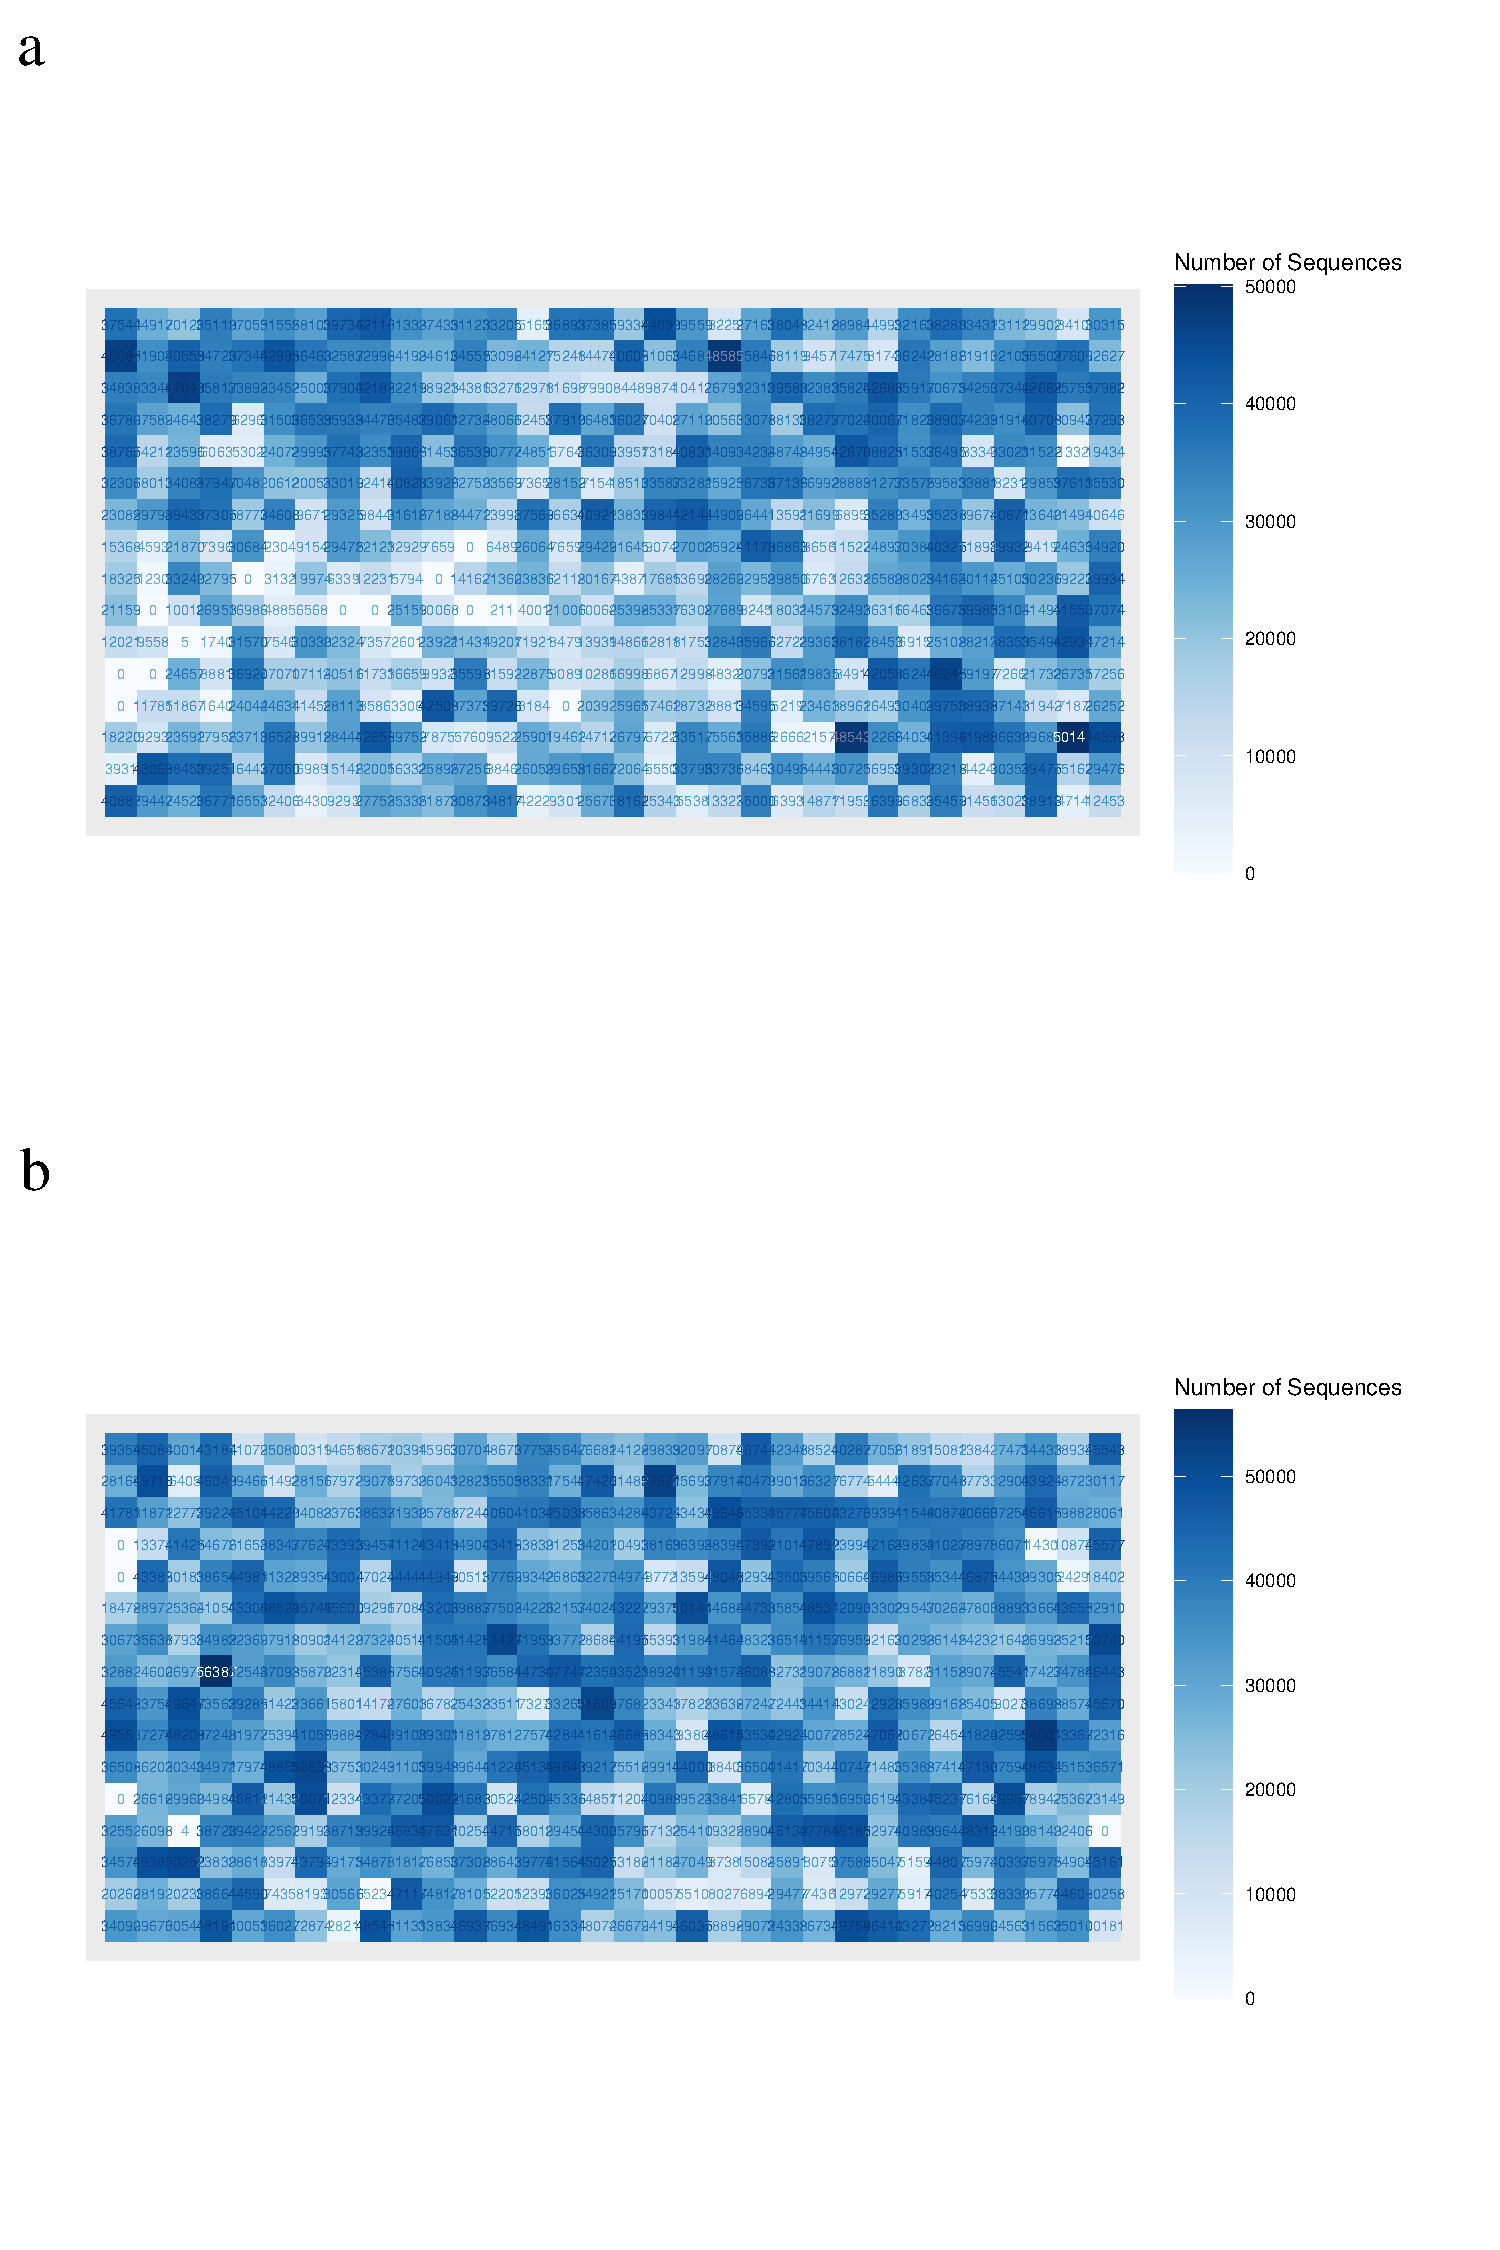
\includegraphics[page=1,trim={0 13cm 0 0},scale = 0.45]{Figures/ONTTargetedTranscriptome.pdf}
	\end{center}
	\captionsetup{width=0.95\textwidth}
	\caption[ONT sequencing channel activity for targeted profiling of the rTg4510 cortex]%
	{\textbf{High sequencing channel activity from nanopore sequencing of the rTg4510 cortex after target enrichment.} Shown is a spatial heatmap representation of channel productivity for \textbf{(A)} batch 2 (sequencing yield = 16.9Gb) and \textbf{(B)} batch 3 (sequencing yield = 22.8Gb). Each square is a channel that contains 4 nanopore nanopore, and the productivity is determined by the number of DNA sequences (represented here with a colour density from white to dark blue) that translocates through each pore in the duration of a given run. A contrast in activity can be seen across both runs: a concentrated patch of inactive channels(white box, 0 reads translocated through pore of interest) in the batch 2 run vs more active channels (dark blue, >50,000 reads translocated through pore of interest) in the batch 3 run. Similar amounts of cDNA were loaded into the flow cells (batch 2: 540ng, batch 3: 500ng)}
	\label{fig:ont_targetedseq_channel}
\end{figure}

\begin{figure}[htp]
	\begin{center}
		\includegraphics[page=2,,trim={0 0cm 0cm 10cm},clip, scale = 0.45]{Figures/ONTTargetedTranscriptome.pdf}
	\end{center}
	\captionsetup{width=0.95\textwidth}
	\caption[ONT temporal run performance for targeted profiling]%
	{\textbf{ONT temporal run performance for targeted profiling.} Shown are time-series plots with the \textbf{(A)} number of bases generated per hour over the course of the run for batch 2 and \textbf{(B)} batch 3, and \textbf{(C)} the reads generated cumulatively for batch 2 and \textbf{(D)} batch 3. The reads were classified as "pass" (dark blue) if QV >= 7 and "fail" (light blue) if QV < 7. T50 and T90 refer to the time (hours) at which 50\% and 90\% of the total number of bases were sequenced. Gb - Gigabases}
	\label{fig:ont_targetedtime_performance}
\end{figure}

\newpage
Although the sequencing yield from ONT nanopore sequencing was comparable to Iso-Seq after target enrichment (Iso-Seq: 19.3 - 24.2Gb, ONT: 16.9 - 22.8Gb), we detected significantly more ONT ID reads (range: 12.3M - 16.3M) than Iso-Seq polymerase reads (range: 0.3M - 0.7M) and subsequently more full-length reads per sample (ONT mean basecalled, filtered reads = 918K, range = 667K - 1.32M, \cref{fig:ONT_targeted_run_output}\textbf{A}; Iso-Seq mean PolyA-FLNC reads = 38.7K, range = 16.8K - 77.2K, \cref{fig:isoseq_targeted_run_output}\textbf{A}). The on-target rate from ONT nanopore sequencing was also comparable to that seen in Iso-Seq (\cref{fig:isoseq_targeted_rate}, \cref{fig:ont_targeted_rate}), suggesting that the ONT targeted dataset provides a deeper coverage of the target genes. We suspect that this reflects an inherent difference between the two technologies: an insert (cDNA sequence of interest) would be sequenced multiple times from multiple polymerase passes in Iso-Seq (\cref{fig:Mechanism}\textbf{A}), whereas the same insert would only be sequenced once following translocation in nanopore sequencing (\cref{fig:ONT_Mechanism}\textbf{A}). The yield in Iso-Seq was thus limited by the number of wells available for sequencing (1M ZMWs), whilst the yield in ONT nanopore sequencing was constrained by the amount of material and channel activity, which was easily maximised to ensure high throughput. However, we also observed that this high ONT sequencing yield was achieved at the expense of read accuracy given reads were only sequenced once; the average ONT read accuracy was 90\% (mean Phred Quality = 10; \cref{tab:ont_targetedrun_output}, \cref{fig:ont_targetedlengthquality}\textbf{A,B}) in comparison to the 99.9\% accuracy of Iso-Seq reads. Of note, this low ONT read accuracy was expected and in line with developments of nanopore chemistry at the time of research (summarised in \cref{fig:ONT_advances}).  

Finally, we noted that the number of full-length reads obtained per sample varied within each batch (\cref{fig:ONT_targeted_run_output}\textbf{B}), reflecting the data from Iso-Seq targeted profiling. We also detected slightly more reads for TG than WT mice in both batches (\cref{fig:ONT_targeted_run_output}\textbf{C}, batch 2: Wilcoxon rank sum test, W = 18, P = 0.063; batch 3: Wilcoxon rank sum test, W = 17, P = 0.11), although the difference was not significant at the 5\% level after merging both datasets (Wilcoxon rank sum test, W = 59, P = 0.10, \cref{fig:ONT_targeted_run_output}\textbf{D}). Deeper examination revealed that this variability was not associated with RIN (corr = -0.267, P = 0.284, Spearman's rank) or barcode from multiplexing (corr = -0.058, P = 0.819, Spearman's rank, \cref{fig:ONT_targeted_run_output}), but a reflection of sequencing more TG samples across both runs (batch 2: WT = 4, TG = 5 samples; batch 3: WT = 4, TG = 5 samples). Notably, this was not an issue with Iso-Seq targeted profiling where the number of WT and TG mice was overall balanced after including samples from batch 1. %Nonetheless, this is unlikely to have a significant impact on subsequent differential analysis given that counts are normalised to the sample 

\begin{figure}[]
	\centering
	\includegraphics[page=5,trim={0 27cm 0 0cm},clip,scale = 0.5]{Figures/ONTTargetedTranscriptome.pdf}
	\captionsetup{width=0.95\textwidth}
	\caption[On-target rate of ONT targeted profiling]%
	{\textbf{On-target rate of ONT nanopore targeted sequencing was comparable to Iso-Seq targeted profiling.} Shown is a box-plot of the on-target rate observed in ONT nanopore sequencing, which was similar to that observed in Iso-Seq targeted sequencing (\cref{fig:isoseq_targeted_rate}). Of note, a difference in the on-target rate between WT and TG in both batches is a likely reflection of the sample variability in sequencing (\cref{fig:ONT_targeted_run_output}\textbf{C,D}). WT - Wild-type mice, TG - rTg4510 transgenic mice}
	\label{fig:ont_targeted_rate}
\end{figure}

\begin{figure}[]
	\begin{center}
		\includegraphics[page=3,trim={0 0cm 0cm 11cm},clip, scale = 0.45]{Figures/ONTTargetedTranscriptome.pdf}
	\end{center}
	\captionsetup{width=0.95\textwidth}
	\caption[ONT run performance metrics from targeted profiling of rTg4510 mice]%
	{\textbf{Expected length and quality distribution of ONT basecalled reads.} Shown are histograms displaying the distribution of \textbf{(A)} mean read quality score of batch 2 and \textbf{(B)} batch 3, and \textbf{(C)} read lengths in batch 2 and \textbf{(D)} batch 3. The distribution is shaded by filtering: light blue for failed reads (Q < 7) and dark blue for passed reads (Q >= 7) }
	\label{fig:ont_targetedlengthquality}
\end{figure}

\begin{figure}[!htp]
	\centering
	\includegraphics[page=4,trim={0 0 0 0},clip,scale = 0.55]{Figures/ONTTargetedTranscriptome.pdf}
	\captionsetup{width=0.95\textwidth}
	\caption[ONT sequencing metrics from targeted profiling of rTg4510 mice]%
	{\textbf{The number of reads generated by ONT nanopore targeted sequencing varied by batch and genotype.} Shown are scatter plots of the \textbf{(A)} number of reads generated from the bioinformatics pipeline after basecalling and demultiplexing, \textbf{(B)} number of minus and plus reads for each sample after demultiplexing (see \cref{fig:ONT_cdnatemplate} for structure of ONT read template), and box-plots of the \textbf{(C)} number of filtered basecalled reads by batch and genotype, and \textbf{(D)} by genotype after merging data from both runs. WT - Wild-type mice, TG - rTg4510 transgenic mice}
	\label{fig:ONT_targeted_run_output}
\end{figure}

\clearpage
\subsection{The vast majority of ONT transcripts were lowly abundant and not detected across biological replicates}
Following the ONT bioinformatics pipeline, we detected a total of 1,367,866 isoforms in ONT targeted dataset of which 445,457 isoforms (32.5\%) were annotated to 20 AD-associated genes enriched in rTg4510 cortex (n = 8 WT, n = 10 TG). Filtering these isoforms by expression (minimum 5 reads across 2 samples) using \textit{Talon}, however, drastically reduced the number of isoforms (fold change = -0.988) to 5,947 (1.19\%) isoforms annotated to AD-associated genes. This suggests that the vast number of ONT transcripts were lowly abundant and not reproducibly detected across biological replicates. Nonetheless, we detected almost twice as many AD-associated isoforms (fold change = 1.66) using ONT nanopore sequencing (n = 5,331 isoforms) than Iso-Seq (n = 2,015 isoforms), despite sequencing fewer samples (Iso-Seq: n = 24 samples, ONT = 18 samples). In line with the sequencing yield generated by the respective technologies, this is again a reflection of the inherent differences in the two technologies (described in \cref{ch6: ont_run_performance}). 

In order to compensate the opposing drawbacks of the two long-read targeted sequencing approaches (high accuracy but relatively lower sequencing coverage of Iso-Seq targeted dataset vs relatively lower accuracy but high sequencing coverage of ONT targeted dataset), we merged both targeted datasets using \textit{Gffcompare} to comprehensively characterise the AD-associated target genes in the rTg4510 cortex (depicted in \cref{fig:Targeted_bioinformatics_pipeline} and described in \cref{ch6: methods_quantification}). This strategy further allowed us to perform stringent filtering, while also retaining ONT-derived isoforms detected in the Iso-Seq targeted dataset that would have otherwise been filtered. 

Comparison of the two datasets using custom scripts revealed that the majority of Iso-Seq-derived transcripts were also detected in ONT nanopore sequencing (n = 617 transcripts, 65.4\%), whereas only a relatively small proportion of filtered ONT-transcripts were detected in the Iso-Seq targeted dataset (n = 701 transcripts, 15.1\%) (\cref{fig:ont_isoseq_venn}). Examination of the unique filtered ONT-derived transcripts revealed them to be shorter (W = 3.14 x 10\textsuperscript{6}, P = 4.0 x 10\textsuperscript{-125}, \cref{fig:ontvsisoseq_description}\textbf{A}) and with fewer exons (W = 3.03 x 10\textsuperscript{6}, P = 1.37 x 10\textsuperscript{-100},\cref{fig:ontvsisoseq_description}\textbf{B}) than the commonly detected ONT-derived transcripts. In contrast, no difference in isoform length (W = 1.76 x 10\textsuperscript{5}, P = 0.72, \cref{fig:ontvsisoseq_description}\textbf{A}) was observed between the unique and commonly detected Iso-Seq derived transcripts, suggesting that these transcripts might be unique to the remaining samples that were not sequenced with ONT. Finally, we observed that the unique Iso-Seq-derived transcripts and ONT-derived transcripts were more abundant than the commonly detected transcripts (\cref{fig:ontvsisoseq_description}\textbf{C}), suggesting that transcript expression was not a differentiating factor for whether a transcript was detected in one technology and not the other. 

\vspace{2cm}
\begin{figure}[htp]
	\centering
	\vspace{20pt}
	\includegraphics[page=4,trim={0 4cm 0 14cm},clip,scale = 0.75]{Figures/TargetedTranscriptome_LabResults.pdf}
	\captionsetup{width=0.95\textwidth}
	\caption[Finalised output from Iso-Seq and ONT targeted profiling of the rTg4510 cortex]%
	{\textbf{Total number of transcripts detected from Iso-Seq and ONT targeted sequencing.} Shown is a Venn diagram of the total number of transcripts annotated to 20 AD-associated target genes detected in Iso-Seq (shaded red) and ONT (shaded blue) targeted datasets. "ONT filtered" transcripts refer to the subset of ONT transcripts that were retained after \textit{TALON} filtering (minimum 5 reads in at least 2 samples). Transcripts in the overlapping sector were defined as complete exact match (class code: "=") using \textit{Gffcompare}. The green dash encompasses the subset of transcripts from ONT and Iso-Seq targeted datasets that were taken further for downstream annotation and quantification analysis}
	\label{fig:ont_isoseq_venn}
\end{figure}

\begin{figure}[!htp]
	\begin{center}
		\includegraphics[page=4,trim={0 13cm 0 0cm},clip,scale = 0.60]{Figures/ONTvsIsoSeq.pdf}
	\end{center}
	\captionsetup{width=0.95\textwidth}
	\caption[Comparison of commonly-detected and unique isoforms from targeted datasets]%
	{\textbf{Transcripts detected in both Iso-Seq and ONT targeted datasets were more abundant, and longer with more exons than isoforms unique to ONT dataset.} Shown are box-plots of the \textbf{(A)} length, \textbf{(B)} exon number and \textbf{(C)} expression of transcripts annotated to AD-associated genes (target genes) that were either detected in both Iso-Seq and ONT targeted datasets, or unique to the Iso-Seq (n = 24 samples) and ONT dataset (n = 18 samples). "Both" refer to transcripts that are detected in Iso-Seq targeted and ONT targeted dataset, "Iso-Seq" and "ONT" refer to transcripts that are only detected in Iso-Seq and ONT targeted datasets, respectively. The Iso-Seq and ONT transcript expression refer to the respective full-length read count for the associated isoform.}
	\label{fig:ontvsisoseq_description}
\end{figure}

\newpage
\subsection{ONT nanopore sequencing achieves significantly deeper sequencing coverage than Iso-Seq with enrichment of shorter novel transcripts}

Following merging of the two targeted datasets, we detected a total of 6,645 isoforms annotated to the 20 AD-associated target genes (\cref{fig:ont_isoseq_venn}). Among these isoforms, the majority were solely derived from ONT nanopore sequencing (n = 4,630, 69.7\%) with a considerable overlap between the two targeted datasets (n = 1,318, 19.8\%) (\cref{fig:ont_isoseq_venn}). Landscape evaluation of these retained ONT-derived isoforms (\cref{fig:ont_targeted_finalnumberiso}\textbf{A}) revealed a striking contrast to the Iso-Seq targeted dataset (\cref{fig:isoseq_targeted_finalnumberiso}\textbf{A}), with an overwhelming majority of isoforms identified as novel and NNC (n = 4728) with novel combination of splice junctions. Significantly more isoforms were detected across the panel of target genes, particularly \textit{Apoe} with over 2000 isoforms detected. Conversely, \textit{Apoe} was one of the fewer "isoformic" gene in the Iso-Seq targeted dataset with only 69 isoforms detected (\cref{fig:isoseq_targeted_finalnumberiso}\textbf{A}), indicating robust differences between the two targeted datasets.

After further filtering of partial isoforms including 5' degradation products, examination of the AD-associated target isoforms (n = 5,587 isoforms) detected using Iso-Seq and ONT nanopore sequencing revealed a clear difference in isoform length and number of exons. While transcripts in the Iso-Seq targeted dataset were typically sized 2-3kb (mean = 2.38kb, s.d = 1.2kb, range = 0.14 - 10.3kb, \cref{fig:ont_isoseq_description}\textbf{A}) with 10 exons (s.d = 7.87, range = 1 - 50, \cref{fig:ont_isoseq_description}\textbf{B}), we noted a prominent enrichment of short transcripts in the ONT targeted dataset sized 1-2kb (mean = 1.79kb, s.d = 1.45kb, range = 0.153 - 10.7kb, \cref{fig:ont_isoseq_description}\textbf{A}) with 5 exons (s.d = 7.06, range = 1 - 50, \cref{fig:ont_isoseq_description}\textbf{B}). This suggests an over-representation of shorter transcripts in the ONT library, a phenomenon that has been previously reported and may be attributed to premature termination of ONT transcript sequencing\cite{Byrne2017}. However notably, we observed a similar distribution of distance to the nearest annotated CAGE peak (\cref{fig:ont_isoseq_description}\textbf{C}), annotated transcription start sites (\cref{fig:ont_isoseq_description}\textbf{D}) and termination sites (\cref{fig:ont_isoseq_description}\textbf{E}) with ONT-derived transcripts more likely to be annotated within 50bp of a CAGE peak, TSS and TTS. The proportion of isoforms with the presence of a known poly(A) site was also similar between Iso-Seq-derived and ONT-derived transcripts, with high support across all isoform categories (\cref{fig:ont_isoseq_description}\textbf{F}). Indicating transcript completeness at both the 5' and 3' end, these results support the validity of these ONT-derived transcripts. 

Finally, using RNA-Seq data generated on matched samples, we found that 80\% (n = 712, 77.7\%) of transcripts detected in both targeted datasets were supported by RNA-Seq reads. Unsurprisingly, this support was low for transcripts unique to the Iso-Seq targeted dataset (n = 243, 63.9\%), and significantly lower for ONT targeted dataset (n = 305, 6.63\%) - a reflection of the higher sensitivity of ONT targeted sequencing to detect rare novel transcripts and the insufficient coverage of RNA-Seq reads to span the junctions of such rare transcripts. In comparing the gene-expression level deduced from RNA-Seq data vs ONT targeted data, we observed an even stronger correlation (corr = 0.92, P = 1.27 x 10\textsuperscript{-8}, \cref{fig:ont_targeted_finalnumberiso}\textbf{B}) than when the comparison was made with Iso-Seq targeted data (corr = 0.86, P = 1.18 x 10\textsuperscript{-6}, \cref{fig:isoseq_targeted_finalnumberiso}\textbf{B}), a further testament to the deep nanopore sequencing coverage.  

%Examination of these novel transcripts not supported by RNA-Seq revealed them to be less abundant (median expression = XX FL reads) compared to those supported by RNA-Seq (median expression = XX FL reads). Nonetheless for transcripts that could be recapitulated in the Iso-Seq targeted data, there was a significant correlation at the between transcript length, exon number and transcript expression.

\begin{figure}[!htp]
	\begin{center}
		\includegraphics[page=2,trim={0 19cm 0 0cm},clip,scale = 0.60]{Figures/ONTvsIsoSeq.pdf}
	\end{center}
	\captionsetup{width=0.95\textwidth}
	\caption[Isoform landscape of AD-risk genes from ONT targeted profiling]%
	{\textbf{ONT is more sensitive than Iso-Seq with greater power to detect novel transcripts.} Shown is the \textbf{(A)} number of isoforms detected per target gene from the ONT targeted dataset, either classified as known (FSM, ISM) or novel (NIC, NNC), after sequential processing and filtering in the bioinformatics ONT pipeline. \textbf{(B)} A strong correlation was observed between ONT gene expression and RNA-Seq gene expression. ONT gene expression was determined from the summation of full-length read counts of associated transcripts, whereas RNA-Seq gene expression was deduced from the normalised \textit{DESeq} counts of aligned RNA-Seq reads to reference genome\cite{Castanho2020}.}
	\label{fig:ont_targeted_finalnumberiso}
\end{figure}

\begin{figure}[!htp]
	\begin{center}
		\includegraphics[page=3,trim={0 9cm 0 0cm},clip,scale = 0.60]{Figures/ONTvsIsoSeq.pdf}
	\end{center}
	\captionsetup{width=0.95\textwidth}
	\caption[Comparison of Iso-Seq and ONT targeted datasets]%
	{\textbf{While ONT-derived isoforms were generally shorter with fewer exons, the 5' and 3' ends are more within the range of annotated sites and CAGE peaks than Iso-Seq derived isoforms.} Shown are density plots of \textbf{(A)} the distribution of the transcript lengths and \textbf{(B)} exon number in the targeted Iso-Seq (n = 24 samples) and ONT datasets (n = 16 samples). Distance between \textbf{(C)} TSS and closest annotated CAGE peak (a negative value refers to a CAGE peak located upstream of TSS), \textbf{(D)} TSS and reference TSS (a negative value refers to a query start downstream of reference), \textbf{(E)} TTS and reference TSS (a negative value refers to a query end upstream of reference). {(E)} A bar plot of the proportion of isoforms in the Iso-Seq and ONT targeted dataset with a poly(A) site. Percentages denoted in green refer to the proportion of isoforms within the respective category with a poly(A) site. TSS - Transcription start site, TTS - Transcription termination site. Iso-Seq and ONT refer to isoforms from the Iso-Seq and ONT targeted profiling dataset, respectively.}
	\label{fig:ont_isoseq_description}
\end{figure}


\clearpage

\subsection{Characterisation of AS events in AD-associated genes}
The depth of sequencing coverage achieved with target gene enrichment, particularly with ONT nanopore sequencing, enabled us to identify hundreds of novel transcripts across the panel of AD-associated genes (\cref{fig:final_targeted_num}, \cref{tab: merged_targeted_num}). Using custom scripts developed to comprehensively annotate such transcripts (illustrated in \cref{fig:Targeted_isoforms_annotate} and described in \cref{ch6: methods_characterisation}), we identified widespread alternative splicing events (n = 17,826 events, \cref{tab: merged_targeted_ASevents}) in our panel of AD-associated target genes.

In line with our previous findings from global transcriptome profiling of the mouse cortex (\cref{ch4_AS}), we observed widespread usage of alternative 5' and 3' splice site (A5', A3') (n = 8,520 events) followed by exon skipping (n = 6,695 events). Usage of alternative splice sites, defined as a site differing by 10-20bp of the reference splice site, was detected for all AD-associated target genes (\cref{fig:A5A3_targeted}\textbf{A}). While there were gene-specific variations (\cref{fig:A5A3_targeted}\textbf{B}), such as \textit{Vgf} with notable usage of alternative splice sites of the final exon (alternative last exon) (\cref{fig: AS_Examples}\textbf{A}), the majority of genes were dominated by alternative 5' and 3' splice sites of internal exons.

Focusing on internal exons, we detected thousands of AD-associated target isoforms with exon skipping (n = 2,431 isoforms, \cref{fig:ES_targeted}\textbf{A}). Although the vast majority of transcripts were characterised with skipping of several exons, some genes were characterised by significantly more exon skipping events: isoforms annotated to \textit{App} (n = 23 isoforms, \cref{fig: AS_Examples}\textbf{B}) and \textit{Bin1} (n = 21 isoforms, \cref{fig: AS_Examples}\textbf{C}) were characterised with skipping of >10 exons (\cref{fig:ES_targeted}\textbf{B}). In contrast to the initial theory that exon skipping predominantly occurs with "alternative exons" (i.e. exons that are not present in all reference isoforms), deeper investigation revealed that over a third of the total exons skipped (n = 2,591 exons, 38.5\%) were "constitutive" (i.e. exons present in all reference isoforms) (\cref{fig:ES_targeted}\textbf{C}). Furthermore, several genes were characterised with widespread exon skipping; across the 358 isoforms annotated to \textit{Ptk2b}, 93.5\% (n = 29 exons)  of \textit{Ptk2b} exons (n = 31 total exons) were found skipped, the overwhelming majority of which were "constitutive" (n = 28, 96.6\% of skipped exons) (\cref{fig:ES_targeted}\textbf{C}). No correlation was observed between the known number of exons and number of exon skipping events (corr = -0.195, P = 0.409). 

\newpage
Conversely, intron retention (IR) was one of the least observed splicing event characterised (n = 747, 4.19\%), corroborating previous findings from global transcriptome profiling of the mouse cortex (\cref{ch4_AS}). Although the majority of IR-isoforms were characterised with only one distinct IR event (defined by the presence of an exon with retention of an intronic region >100bp from the splice site), several genes were associated with a few novel rare transcripts with multiple IR events (\cref{fig:IR_targeted}\textbf{A}); this was particularly evident in \textit{Abca7} (4 IR events = 1, 3 IR events = 3, \cref{fig: AS_Examples}\textbf{D}). The majority of IR-events were further found to span across at least two exons, with a significant proportion of isoforms characterised with extensive intron retention spanning across 4 exons (\cref{fig:IR_targeted}\textbf{B}). Finally, we found an association between increased intron retention events and transcript expression (\cref{fig:IR_targeted}\textbf{C}), corroborating our findings (described in \cref{ch4: IR}) and previous studies\cite{Braunschweig2014} suggesting that IR is associated with reduced transcript abundance.
%nonsense mediated decay

\newpage
\newgeometry{bottom=2cm, top=2cm}
\begin{figure}[]
	\centering
	\includegraphics[page=8,trim={0 26cm 0 0cm},clip,scale = 0.55]{Figures/ONTvsIsoSeq.pdf}
	\captionsetup{width=0.95\textwidth}
	\caption[Merged isoform landscape from Iso-Seq \& ONT targeted profiling]%
	{\textbf{Targeted profiling of the rTg4510 cortex identify hundreds of novel transcripts annotated to AD-associated target genes.} Shown is a bar plot of the final number of isoforms detected per AD-risk gene after merging Iso-Seq and ONT targeted datasets.}
	\label{fig:final_targeted_num}
\end{figure}

\vspace{1cm}
\begin{table}[]
	\centering
	\captionsetup{width=0.95\textwidth}
	\caption[Overview of the isoform landscape of AD-associated genes]%
	{\textbf{Overview of the isoform landscape of AD-associated genes.} Tabulated is a summary of the isoform landscape per AD-associated gene after targeted profiling of the rTg4510 cortex. Splice junctions were defined by the two pairs of dinucleotides present at the exon-intron boundary, and any other combinations aside from GT-AG, GC-AG and AT-AC pairs were considered non-canonical.}
	\label{tab: merged_targeted_num}
	\centering
	\setlength\tabcolsep{5pt} %reduced margin size in table
	\begin{tabular}{@{}cccccccc@{}}
		\toprule
		\multirow{3}{*}{Genes} & \multicolumn{7}{c}{Number of Isoforms}                                                                    \\ \cmidrule(l){2-8} 
		& \multicolumn{3}{c}{Classification} & \multicolumn{2}{c}{Coding potential} & \multicolumn{2}{c}{Splice junctions} \\ \cmidrule(l){2-8} 
		& All      & Known      & Novel      & Coding          & Non-Coding         & Canonical     & Non canonical    \\ \midrule
		\textit{Abca1}  & 7    & 1  & 2    & 7    & 0   & 7   & 0    \\
		\textit{Abca7}  & 41   & 3  & 34   & 40   & 1   & 41  & 0    \\
		\textit{Ank1}   & 17   & 9  & 3    & 15   & 2   & 17  & 0    \\
		\textit{Apoe}   & 2006 & 10 & 1987 & 1978 & 28  & 980 & 1030 \\
		\textit{App}    & 466  & 9  & 398  & 451  & 15  & 410 & 56   \\
		\textit{Bin1}   & 368  & 6  & 348  & 366  & 2   & 347 & 21   \\
		\textit{Cd33}   & 41   & 5  & 34   & 39   & 2   & 43  & 1    \\
		\textit{Clu}    & 773  & 7  & 756  & 757  & 16  & 457 & 316  \\
		\textit{Fus}    & 236  & 10 & 200  & 223  & 13  & 219 & 22   \\
		\textit{Fyn}    & 50   & 5  & 40   & 48   & 2   & 50  & 0    \\
		\textit{Mapt}   & 140  & 9  & 113  & 115  & 25  & 136 & 5    \\
		\textit{Picalm} & 144  & 12 & 126  & 117  & 27  & 144 & 2    \\
		\textit{Ptk2b}  & 563  & 7  & 528  & 553  & 10  & 413 & 150  \\
		\textit{Rhbdf2} & 5    & 1  & 4    & 5    & 0   & 5   & 0    \\
		\textit{Snca}   & 622  & 3  & 614  & 220  & 402 & 468 & 154  \\
		\textit{Sorl1}  & 113  & 3  & 12   & 104  & 9   & 113 & 1    \\
		\textit{Tardbp} & 127  & 21 & 80   & 105  & 22  & 124 & 3    \\
		\textit{Trem2}  & 140  & 3  & 61   & 63   & 77  & 66  & 4    \\
		\textit{Trpa1}  & 4    & 1  & 3    & 3    & 1   & 4   & 0    \\
		\textit{Vgf}    & 90   & 2  & 86   & 52   & 38  & 19  & 71   \\ \bottomrule
	\end{tabular}
\end{table}

\begin{figure}[]
	\centering
	\includegraphics[page=9,trim={0 26cm 0 0cm},clip,scale = 0.55]{Figures/ONTvsIsoSeq.pdf}
	\captionsetup{width=0.95\textwidth}
	\caption[Merged splicing landscape from Iso-Seq and ONT targeted profiling]%
	{\textbf{Targeted profiling of the rTg4510 cortex identify widespread usage of splicing events.} Shown is a bar plot of proportion of alternative splicing events identified per AD-risk gene after merging Iso-Seq and ONT targeted datasets.}
	\label{fig:AS_targeted}
\end{figure}

\begin{table}[]
	\centering
	\captionsetup{width=0.95\textwidth}
	\caption[Characterisation of alternative splicing events in AD-risk genes]%
	{\textbf{Characterisation of alternative splicing events in AD-risk genes.} Tabulated is a summary of alternative splicing events per AD-risk gene after targeted profiling of the rTg4510 cortex.}
	\label{tab: merged_targeted_ASevents}
	\setlength\tabcolsep{9pt} %reduced margin size in table
	\begin{tabular}{@{}ccccccccc@{}}
		\toprule
		\multirow{2}{*}{Genes} & \multicolumn{2}{c}{Number of  Transcripts} & \multicolumn{6}{c}{Number of Events} \\ \cmidrule(l){2-9} 
		& ES  & IR  & A5A3 & AF & AP  & AT & ES   & IR  \\ \midrule
		\textit{Abca1}  & 2   & 2   & 5    & 0  & 4   & 0  & 3    & 2   \\
		\textit{Abca7}  & 9   & 25  & 27   & 0  & 28  & 0  & 9    & 54  \\
		\textit{Ank1}   & 9   & 0   & 20   & 0  & 2   & 0  & 17   & 0   \\
		\textit{Apoe}   & 125 & 8   & 4054 & 0  & 40  & 2  & 156  & 16  \\
		\textit{App}    & 406 & 13  & 752  & 0  & 218 & 28 & 1872 & 17  \\
		\textit{Bin1}   & 290 & 52  & 295  & 0  & 101 & 9  & 1072 & 109 \\
		\textit{Cd33}   & 18  & 23  & 49   & 0  & 3   & 0  & 18   & 52  \\
		\textit{Clu}    & 270 & 119 & 844  & 0  & 169 & 0  & 660  & 241 \\
		\textit{Fus}    & 103 & 32  & 200  & 0  & 29  & 3  & 196  & 79  \\
		\textit{Fyn}    & 44  & 0   & 46   & 0  & 13  & 2  & 98   & 0   \\
		\textit{Mapt}   & 115 & 24  & 97   & 0  & 45  & 18 & 527  & 44  \\
		\textit{Picalm} & 83  & 0   & 114  & 0  & 81  & 1  & 148  & 0   \\
		\textit{Ptk2b}  & 358 & 33  & 632  & 0  & 301 & 0  & 873  & 57  \\
		\textit{Rhbdf2} & 2   & 0   & 6    & 0  & 2   & 0  & 2    & 0   \\
		\textit{Snca}   & 483 & 14  & 784  & 0  & 16  & 2  & 917  & 14  \\
		\textit{Sorl1}  & 3   & 0   & 193  & 0  & 99  & 96 & 6    & 0   \\
		\textit{Tardbp} & 8   & 38  & 104  & 0  & 0   & 2  & 10   & 42  \\
		\textit{Trem2}  & 28  & 12  & 118  & 0  & 2   & 0  & 36   & 18  \\
		\textit{Trpa1}  & 1   & 2   & 1    & 0  & 1   & 0  & 1    & 2   \\
		\textit{Vgf}    & 74  & 0   & 179  & 0  & 6   & 1  & 74   & 0   \\ \bottomrule
	\end{tabular}
\end{table}

\begin{figure}[]
	\centering
	\includegraphics[page=10,trim={0 20cm 0 0cm},clip,scale = 0.55]{Figures/ONTvsIsoSeq.pdf}
	\captionsetup{width=0.95\textwidth}
	\caption[Characterisation of alternative 5' and 3' splice sites in AD-risk genes]%
	{\textbf{Extensive usage of alternative 5' and 3' splice sites in AD-risk genes.} Shown are bar plots of the \textbf{(A)} number of isoforms annotated to AD-risk genes with alternative 5' (A5') and alternative 3' (A3') splice sites, further classified by the relative location of the novel splice site to the reference splice site, and of the \textbf{(B)} proportion of isoforms with alternative splice sites in the first, internal and last exons.}
	\label{fig:A5A3_targeted}
\end{figure}

\begin{figure}[]
	\centering
	\includegraphics[page=6,trim={0 20cm 0 0cm},clip,scale = 0.55]{Figures/ONTvsIsoSeq.pdf}
	\captionsetup{width=0.95\textwidth}
	\caption[Characterisation of exon skipping events in AD-risk genes]%
	{\textbf{Extensive occurrence of exon skipping events in AD-risk genes.} Shown are bar plots of the \textbf{(A)} number of isoforms annotated to AD-risk genes with exon skipping events, \textbf{(B)} number of unique exons skipped. Constitutive exons refer to exons that are present in all known reference isoforms.}
	\label{fig:ES_targeted}
\end{figure}

\begin{figure}[]
	\centering
	\includegraphics[page=11,trim={0 0cm 0 0cm},clip,scale = 0.55]{Figures/ONTvsIsoSeq.pdf}
	\captionsetup{width=0.95\textwidth}
	\caption[Characterisation of intron retention events in AD-risk genes]%
	{\textbf{Relatively few occurrence of intron retention events, which typically spanned across two exons in lowly-expressed transcripts.} Shown is \textbf{(A)} a bar-plot of the number of isoforms annotated to AD-associated gene with intron retention events, and \textbf{(B)} the number of exons for which intron retention events span across, and \textbf{(C)} a box-plot of the expression of transcripts with multiple intron retention events. Transcript expression is deduced from normalised ONT full-length read counts.}
	\label{fig:IR_targeted}
\end{figure}
\restoregeometry

\newgeometry{left=2cm, right = 2cm, bottom = 2cm, top = 2cm}
\begin{landscape}
\begin{figure}[]
	\centering
	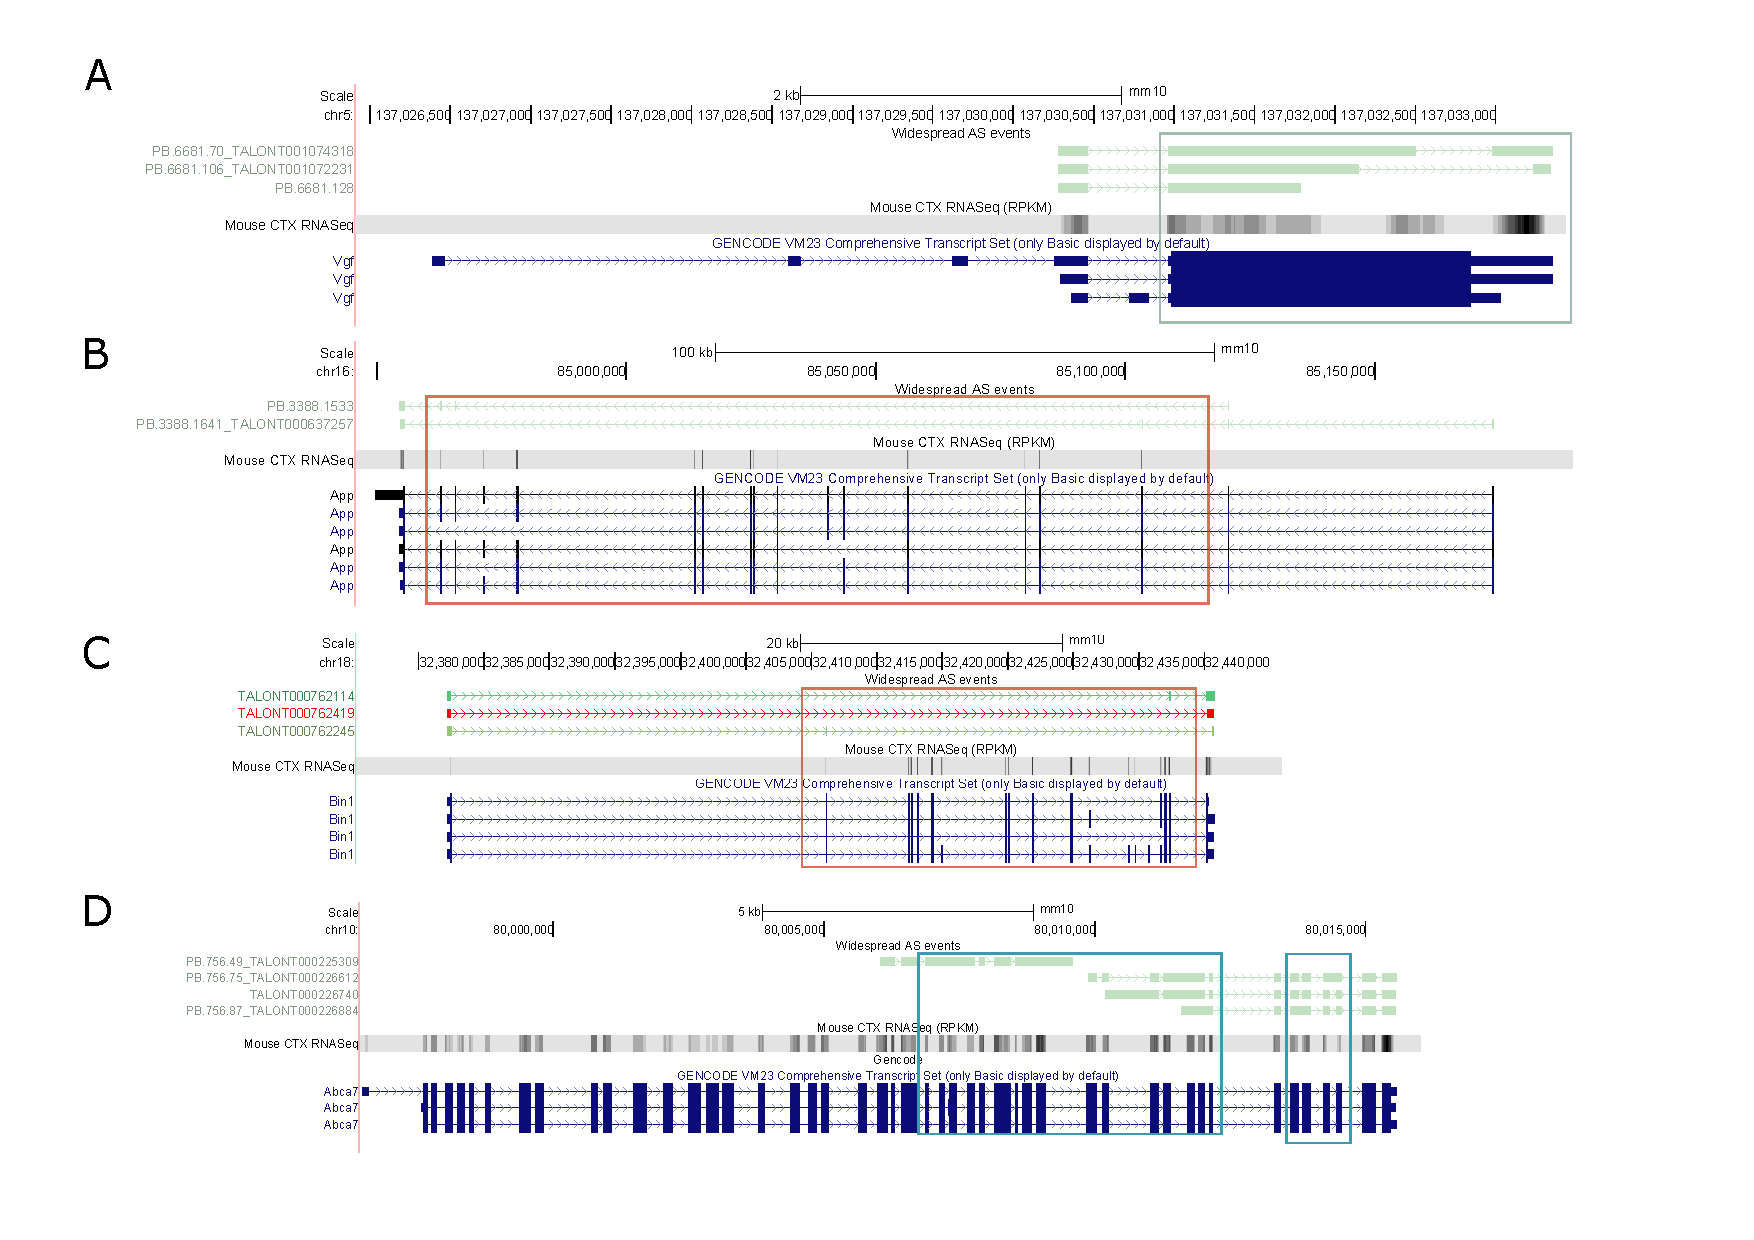
\includegraphics[page=1,trim={0 1.5cm 0 1cm},clip,scale = 0.85]{Figures/TargetGenesASExamples.pdf}
	\captionsetup{width=1.25\textwidth}
	\caption[Examples of AD-risk genes with extensive usage of splicing events]%
	{\textbf{Examples of AD-risk genes with extensive usage of splicing events.} Shown are UCSC genome browser tracks of \textbf{(A)} three \textit{Vgf}-associated isoforms with usage of alternative splice sites in last exon (green box), \textbf{(B)} two \textit{App}-associated isoforms \textbf{(C)} three \textit{Bin1}-associated isoforms with multiple exons skipped (>15 exons, red box), and \textbf{(D)} four \textbf{Abca7}-associated isoforms with multiple intron retention events (blue box).}
	\label{fig: AS_Examples}
\end{figure}
\end{landscape}
\restoregeometry

\clearpage
\subsection{Comprehensive characterisation of AD-associated genes} 
\label{ch6: target_gene_annotation}
This section details comprehensive transcript annotations from the merged Iso-Seq and ONT targeted long-read datasets generated for 20 AD-associated genes in the rTg4510 mouse entorhinal cortex. A series of UCSC genome browser tracks and cluster dendrogram were generated for visualisation each target gene. Examples of these can be found in \cref{fig:eg_heatmap} and \cref{fig:eg_heatmap}, respectively. 

\vspace{1cm}
\begingroup
\parindent=0em
\etocsettocstyle{\rule{\linewidth}{\tocrulewidth}\vskip0.5\baselineskip}{\rule{\linewidth}{\tocrulewidth}}
\etocsetnexttocdepth{5}
\localtableofcontents 
\endgroup

\begin{figure}[htp]
	\centering
	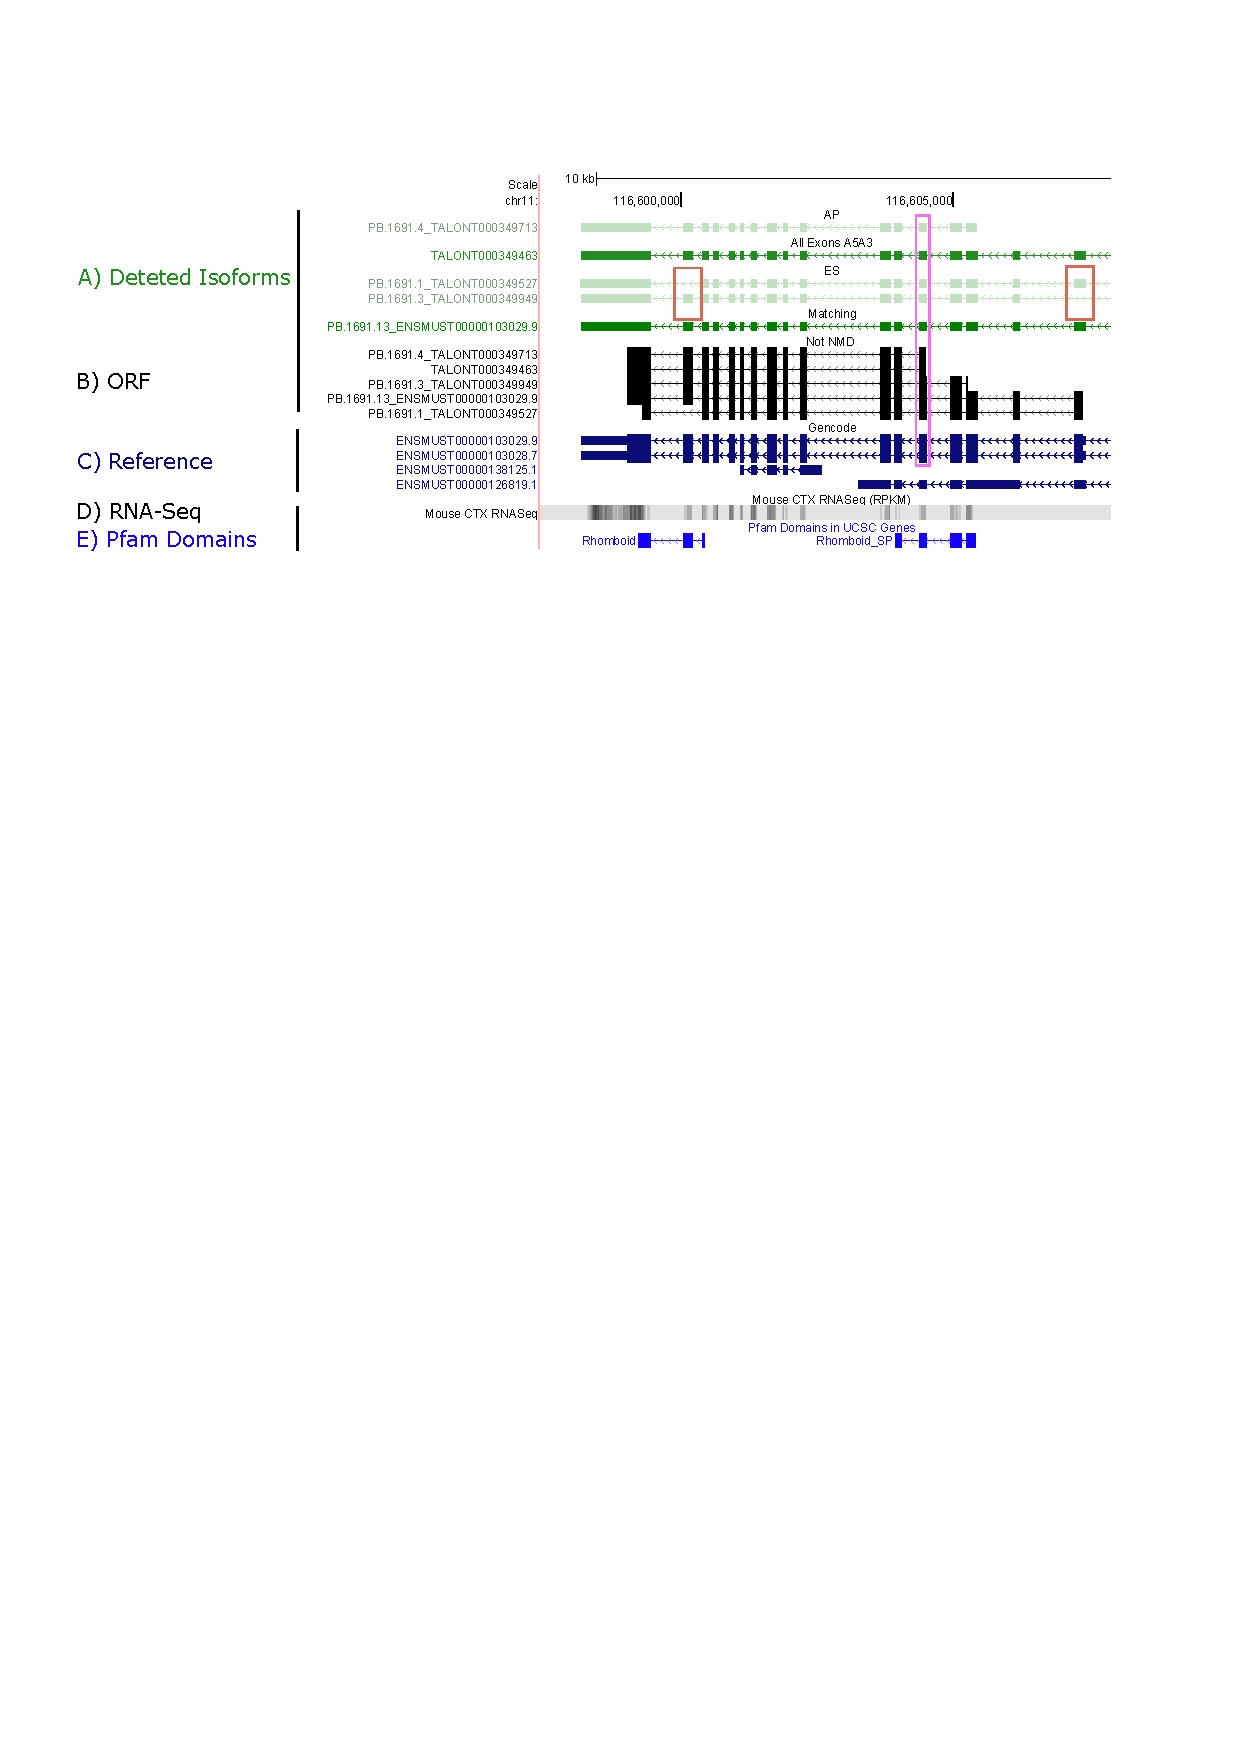
\includegraphics[page=1,trim={1cm 19cm 0 0},scale = 0.85]{Figures/ExamplePlots.pdf}
	\captionsetup{width=0.95\textwidth, singlelinecheck=off}
	\caption[Example of a UCSC genome browser track of an AD-risk target gene]%
	{\textbf{Example of a UCSC genome browser track of an AD-risk target gene.} Shown is an example of a UCSC genome browser track of isoforms annotated to \textit{Cd33}. Tracks are typically displayed in four panels in the following order: 
	\begin{enumerate}[label=\textbf{(\Alph*)}]
		\item isoforms detected from the merged targeted dataset of the rTg4510 cortex (n = 12 WT, n = 12 TG) coloured by protein coding potential (green for protein-coding, red for non-protein coding) and shaded by abundance. Isoforms detected using both Iso-Seq and ONT nanopore sequencing are labelled with two IDs separated by an underscore ("\_") with the first and second part denoting to the PacBio and ONT isoform IDs, respectively. Conversely, isoforms unique to the Iso-Seq and ONT targeted datasets are labelled as "PB.XXX" and "TALONTXXXX", respectively.   
		\item open reading frame (black) predicted for isoforms using \textit{CPAT} 
		\item known isoforms (blue) from existing reference mouse annotations (mm10, GENCODE vM22)
		\item RNA-Seq data from global transcriptome profiling of the rTg4510 cortex\cite{Castanho2020} (n = 30 WT, n = 29 TG)
		\item Pfam domains from the pfam database - a large curated collection of protein families and domains - as part of UCSC genome browser tracks	
		\\ \\	
	\end{enumerate} 

	Of note, only selected isoforms of interest are displayed given the extremely large number of isoforms detected from targeted sequencing. For genes supplemented with several UCSC tracks, some of the tracks exclude display of RNA-Seq and Pfam domains. Furthermore, some tracks are presented in "squish" mode with compression of intronic regions and exon-only display to ease visualisation. 
	}   
	\label{fig:eg_track}
\end{figure}

\begin{figure}[htp]
	\centering
	\includegraphics[page=2,trim={1cm 15cm 0 2cm},scale = 0.85]{Figures/ExamplePlots.pdf}
	\captionsetup{width=0.95\textwidth, singlelinecheck=off}
	\caption[Example of a cluster dendrogram of an AD-risk target gene]%
	{\textbf{Example of a cluster dendrogram of an AD-risk target gene.} Shown is an example of a cluster dendrogram of all detected isoforms annotated to \textit{Cd33}. Each row corresponds to an isoform and each column represents an exon. The isoforms are further clustered by exonic structure and two key splicing events - exon skipping (ES) and intron retention (IR), to ease visualisation. Providing an overview of the isoform landscape, we can evidently see occurrence of intron retention events (box blue) in almost all exons except for exon 1 and 3, and prevalent skipping of exon 8. 
	}   
	\label{fig:eg_heatmap}
\end{figure}

\clearpage
\subsubsection{Abca1}
The ATP-binding cassette transport A1 gene, \textit{ABCA1}, is hypothesised to be a risk gene for AD as a consequence of its role in cholesterol transport and lipid metabolism\cite{Nordestgaard2015}. Involved in ApoE lipidation, Abca1 has been shown to facilitate A$\beta$ clearance in mouse models\cite{Fitz2012}. 

Spanning over 129kb on chromosome 4, the mouse \textit{Abca1} gene is characterised with 50 unique exons and two known isoforms. Despite the large number of exons, we only detected 7 isoforms annotated to \textit{Abca1} in the rTg4510 mouse cortex (\cref{fig:abca1}\textbf{A}), including the known long canonical isoform (Abca1-201, ENSMUST00000030010.3). While most of the isoforms were significantly shorter, we identified a long isoform that spanned the length of Abca1-201 (\cref{fig:abca1}\textbf{A}). Sequenced using both Iso-Seq and ONT technologies, this isoform differed from Abca1-201 with skipping of exons 24 and 35 (\cref{fig:abca1}\textbf{B}) and the presence of a novel exon located between exons 24 and 25 (\cref{fig:abca1}\textbf{C}). Skipping of exon 35, which partially encodes the ABC2 membrane 3 (\textit{Abca1} transmembrane domain), was also observed in one of the shorter isoforms. Embedded in the membrane bilayer, the \textit{Abca1} transmembrane domain is involved in substrate transport across the membrane. While it is less conserved than the ATP-binding domain, the structure of the transmembrane domain is determines the specificity and binding affinity of substrates. ORF prediction showed that skipping of exon 35 shortened but maintained the open reading frame, and inclusion of the novel exon did not translate to additional protein domains. In contrast to this long isoform, we identified two shorter isoforms with intron retention in the last exon (\cref{fig:abca1}\textbf{A,B}). ORF prediction of such transcripts showed a shortened but similar reading frame with no prediction of nonsense-mediated decay. 

\newgeometry{left=2cm, right = 2cm, bottom = 2cm, top = 2cm}
\begin{landscape}
	\begin{figure}[htp]
		\centering
		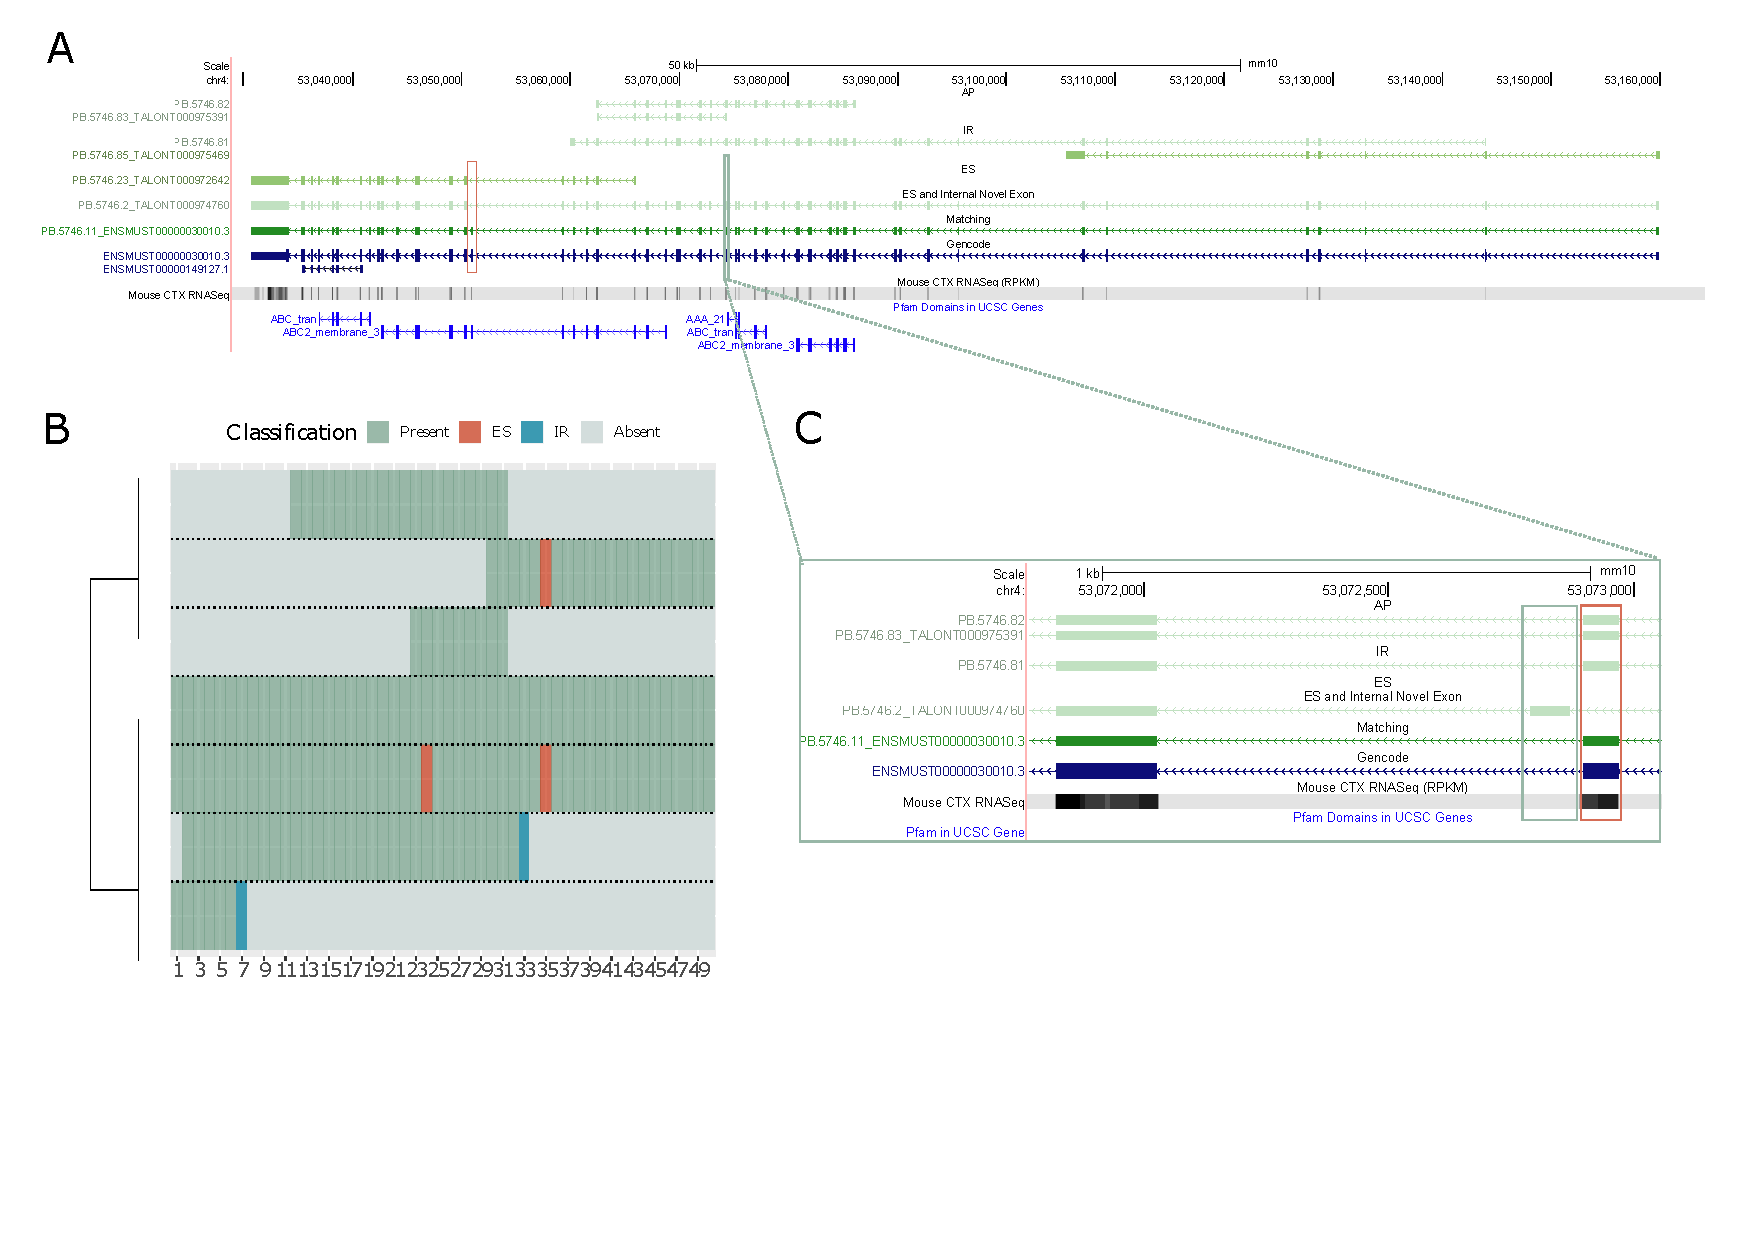
\includegraphics[page=1,trim={0 4cm 0 0},scale = 0.85]{Figures/TargetGenes_Annotation_Landscape.pdf}
		\captionsetup{width=1.3\textwidth}
		\caption[Characterisation of the \textit{Abca1} isoform landscape in the rTg4510 mouse cortex]%
		{\textbf{Characterisation of the \textit{Abca1} isoform landscape in the rTg4510 cortex.} Shown are \textbf{(A)} a UCSC genome browser track of isoforms annotated to \textit{Abca1}, \textbf{(B)} a cluster dendrogram for an overview of the \textit{Abca1} isoform landscape, and \textbf{(C)} a zoomed-in track showing skipping of exon 24 (boxed red) and inclusion of a novel exon (boxed green).}   
		\label{fig:abca1}
	\end{figure}
\end{landscape}
\restoregeometry

\newpage
\subsubsection{Abca7}
Another member of the ATP-binding cassette transporters, the ATP-binding cassette transport A7 gene, \textit{ABCA7}, is also a risk gene for AD with the identification of both common and rare variants associated with the disease\cite{Steinberg2015,Cuyvers2015,Guennec2016}. Analogous to ABCA1, ABCA7 is involved in regulating lipid transport and metabolism, including ApoE lipidation\cite{DeRoeck2019a}. 

Spanning 20kb on chromosome 10, the mouse \textit{Abca7} gene is characterised with 50 exons and three known isoforms. In contrast to \textit{Abca1}, we detected 41 isoforms associated with \textit{Abca7}. A reflection of the almost-identical structure of the three known isoforms (\cref{fig:abca7}\textbf{D}), we identified four novel isoforms that spanned the full-length of the gene, shared similar exonic structure, differing by minor wobble (<10bp) at the splice sites (\cref{fig:abca7}\textbf{D}). In contrast to these long isoforms, we also detected significantly shorter isoforms that broadly fell into 2 categories: i) isoforms that preserved the exonic structure at the 5'-end with an alternative last exon characterised with intron retention (n = 5 isoforms, 12.2\%), and ii) isoforms with an alternative first exon and a 3'-end characterised with exon skipping and intron retention events (n = 23, 56\%) (\cref{fig:abca7}\textbf{A}). Exon skipping was further found exclusive to exon 31 (n = 1, 2.4\%) and exon 32 (n = 8, 19.5\%) (\cref{fig:abca7}\textbf{B}), both of which partially encode the ABC2 membrane 3 (\textit{Abca7} transmembrane domain)\cite{DeRoeck2019a}. Intron retention was also particularly enriched between exons 37 and exon 39 (\cref{fig:abca7}\textbf{C}), both of which also encode the ABC2 membrane 3. Analogous in structure to Abca1, the transmembrane domain is involved in substrate transport across the membrane lipid bilayer by undergoing a conformational change. 
%check AUG promoter 

\newgeometry{left=1cm, right = 1cm, bottom = 2cm, top = 2cm}
\begin{landscape}
	\begin{figure}[htp]
		\centering
		\captionsetup{width=1.3\textwidth}
		\includegraphics[page=2,trim={0 1.5cm 0 0},scale = 0.85]{Figures/TargetGenes_Annotation_Landscape.pdf}
		\caption[Characterisation of the \textit{Abca7} isoform landscape]%
		{\textbf{Characterisation of the \textit{Abca7} isoform landscape in the rTg4510 cortex.} Shown are \textbf{(A)} a cluster dendrogram for an overview of the \textit{Abca7} isoform landscape, \textbf{(B)} a bar-plot of the number of isoforms with exon skipping, \textbf{(C)} the number of isoforms with intron retention (IR), and \textbf{(D)} a UCSC genome browser track of isoforms annotated to \textit{Abca7}. Intron retention events are further classified as "IR" it occurs at one exon or "IR Match" if it spans across multiple exons. }    
		\label{fig:abca7}
	\end{figure}
\end{landscape}
\restoregeometry

\subsubsection{Ank1} 
\label{ch6: ank1}
Recent epigenome-wide association studies (EWAS) have identified a number of genetic loci at which variable DNA methylation is associated with increased risk of AD pathology\cite{Smith2019, Lunnon2014}. One locus that is consistently hypermethylated in AD post-mortem brain tissues resides in \textit{ANK1}, a gene that encodes an integral membrane involved in mediating attachment of membrane proteins to the underlying cytoskeleton\cite{Smith2019, Lunnon2014}. Important for key activities such as cell mobility and proliferation, ANK1 is associated with multiple isoforms with varying lengths and affinity for target membrane proteins.

Spanning over 175kb on chromosome 8, the mouse \textit{Ank1} gene is characterised with 46 exons and 17 known isoforms. In our dataset, \textit{Ank1} stood out from the panel of target genes for enrichment of the significantly shorter known isoforms (\cref{fig:ank1}\textbf{A, B}). While we detected several of the longer known isoforms (n = 4, 23.5\%, length = 6.5 - 8.2kb), the majority of the 17 \textit{Ank1}-associated isoforms were less than \textasciitilde 2kb (n = 11, 64.7\%) in alignment with the shorter known \textit{Ank1}-associated isoforms (sAnk1) that span the 3'end. The two most abundant isoforms also corresponded to one of the short known isoforms (Ank1-208, ENSMUST00000121075.7) and the short non-coding isoform (Ank1-211, ENSMUST00000130311.1). Expression of such short, truncated isoforms have been previously found to be specific to striated muscles and is driven by the activity of second alternative promoter \cite{Gallagher1998}. Notably, recent studies have identified a type 2 diabetes risk allele that increases promoter activity and sAnk1 expression\cite{Yan2016}.  %Although we are unable to rule out the technical limits of sequencing the longer transcripts, given that \textit{Ank1} is one of the longer genes from the panel of target genes,  

Aside from the length disparities among the isoforms detected, we found that the splicing pattern was generally conserved across the gene with consistent skipping of certain exons, notably exons 44 and 47 (\cref{fig:ank1}\textbf{C}). Both exons were present in the majority of known isoforms (n = 11 isoforms, 64.7\%), and did encode for any ankyrin repeat domains. Strikingly ORF predictions indicated that while exon 44 skipping maintained the reading frame, inclusion of this exon resulted in a stop codon (\cref{fig:ank1}\textbf{D}). Isoforms without exon 44 skipping were subsequently predicted for nonsense-mediated decay. 

\newgeometry{left=1cm, right = 1cm, bottom = 2cm, top = 2cm}
\begin{landscape}
	\begin{figure}[htp]
		\centering
		\captionsetup{width=1.3\textwidth}
		\includegraphics[page=3,trim={0 1.5cm 0 0},scale = 0.85]{Figures/TargetGenes_Annotation_Landscape.pdf}
		\caption[Characterisation of \textit{Ank1} isoforms]%
		{\textbf{Characterisation of \textit{Ank1} isoforms in the rTg4510 cortex.} Shown are \textbf{(A)} a cluster dendrogram for an overview of the \textit{Ank1} isoform landscape, \textbf{(B)} a UCSC genome browser track of isoforms annotated to \textit{Ank1}. Isoforms with a black box and indicated by a black arrow contain exon 44 and are subsequently not predicted for nonsense-mediated decay (NMD). \textbf{(C)} A bar-plot of the number of isoforms with exon skipping, and \textbf{(D)} a zoomed-in track showing isoforms with exon 44 inclusion resulting in truncated reading frames and products predicted for nonsense-mediated decay. }    
		\label{fig:ank1}
	\end{figure}
\end{landscape}
\restoregeometry

\newpage
\subsubsection{Apoe}
\label{ch6: apoe}
To date, inheritance of the $\epsilon$4-allele of \textit{APOE}, which encodes the apolipoprotein E, is the strongest risk factor for late-onset AD (detailed in \cref{aetiologyAD}). Involved in regulating lipid homeostasis, ApoE facilitates lipid transport essential for CNS development and maintenance. Characterised with three well-known human isoforms, ApoE exhibit isoform-specific activity and binding affinity for substrates, including $\beta$-amyloid peptides\cite{Jablonski2021}. 

Despite only containing 4 exons (7 if the 3 alternative exons are included) and spanning just over 3kb on chromosome 7, the mouse gene \textit{Apoe} was the most "isoformic" gene among our panel of AD-associated target genes; we detected an overwhelming total of 2,006 isoforms. While the majority of isoforms contained all 4 exons (n = 1,390, 69.2\%) (\cref{fig:apoe}\textbf{A}), a deeper examination of \textit{Apoe} revealed complex variations of exon 6 (last/penultimate exon depending on the reference isoform of interest) and the 3'UTR (\cref{fig:apoe}\textbf{B}). Notably, this 831bp exon encodes the apolipoprotein domain that binds to lipids.  Supported by RNA-Seq data from matched samples, these variations included usage of alternative 5' and 3' splice sites of this exon, or of matched 5' and 3' end sites but skipping within the exon resulting in two enclosed exons (\cref{fig:apoe}\textbf{B}). Noteworthy, one of the known isoforms, Apoe-202 (ENSMUST00000167646.8) was also characterised with this "internal exon skipping" phenomenon.

In contrast to exon 6, the other exons were relatively conserved with significantly fewer variations of 5' and 3' splice sites (\cref{fig:apoe}\textbf{D}). However, unlike exon 6 which was present in nearly all isoforms, we detected skipping events of such exons (\cref{fig:apoe}\textbf{E}): exon 4 (n = 61 isoforms, 48.8\% of isoforms with ES) and exon 5 (n = 89, 71.2\% of isoforms with ES). Despite this widespread isoform diversity, we only detected four isoforms that contained the known alternative first exon present in one of the known isoforms, Apoe-204 (ENSMUST00000172983.7). Notably, one of these isoforms (TALONT00166063) was characterised with both the first canonical exon and the alternative first exon, indicating that these exons are not mutually exclusive. 

\begin{figure}[htp]
	\centering
	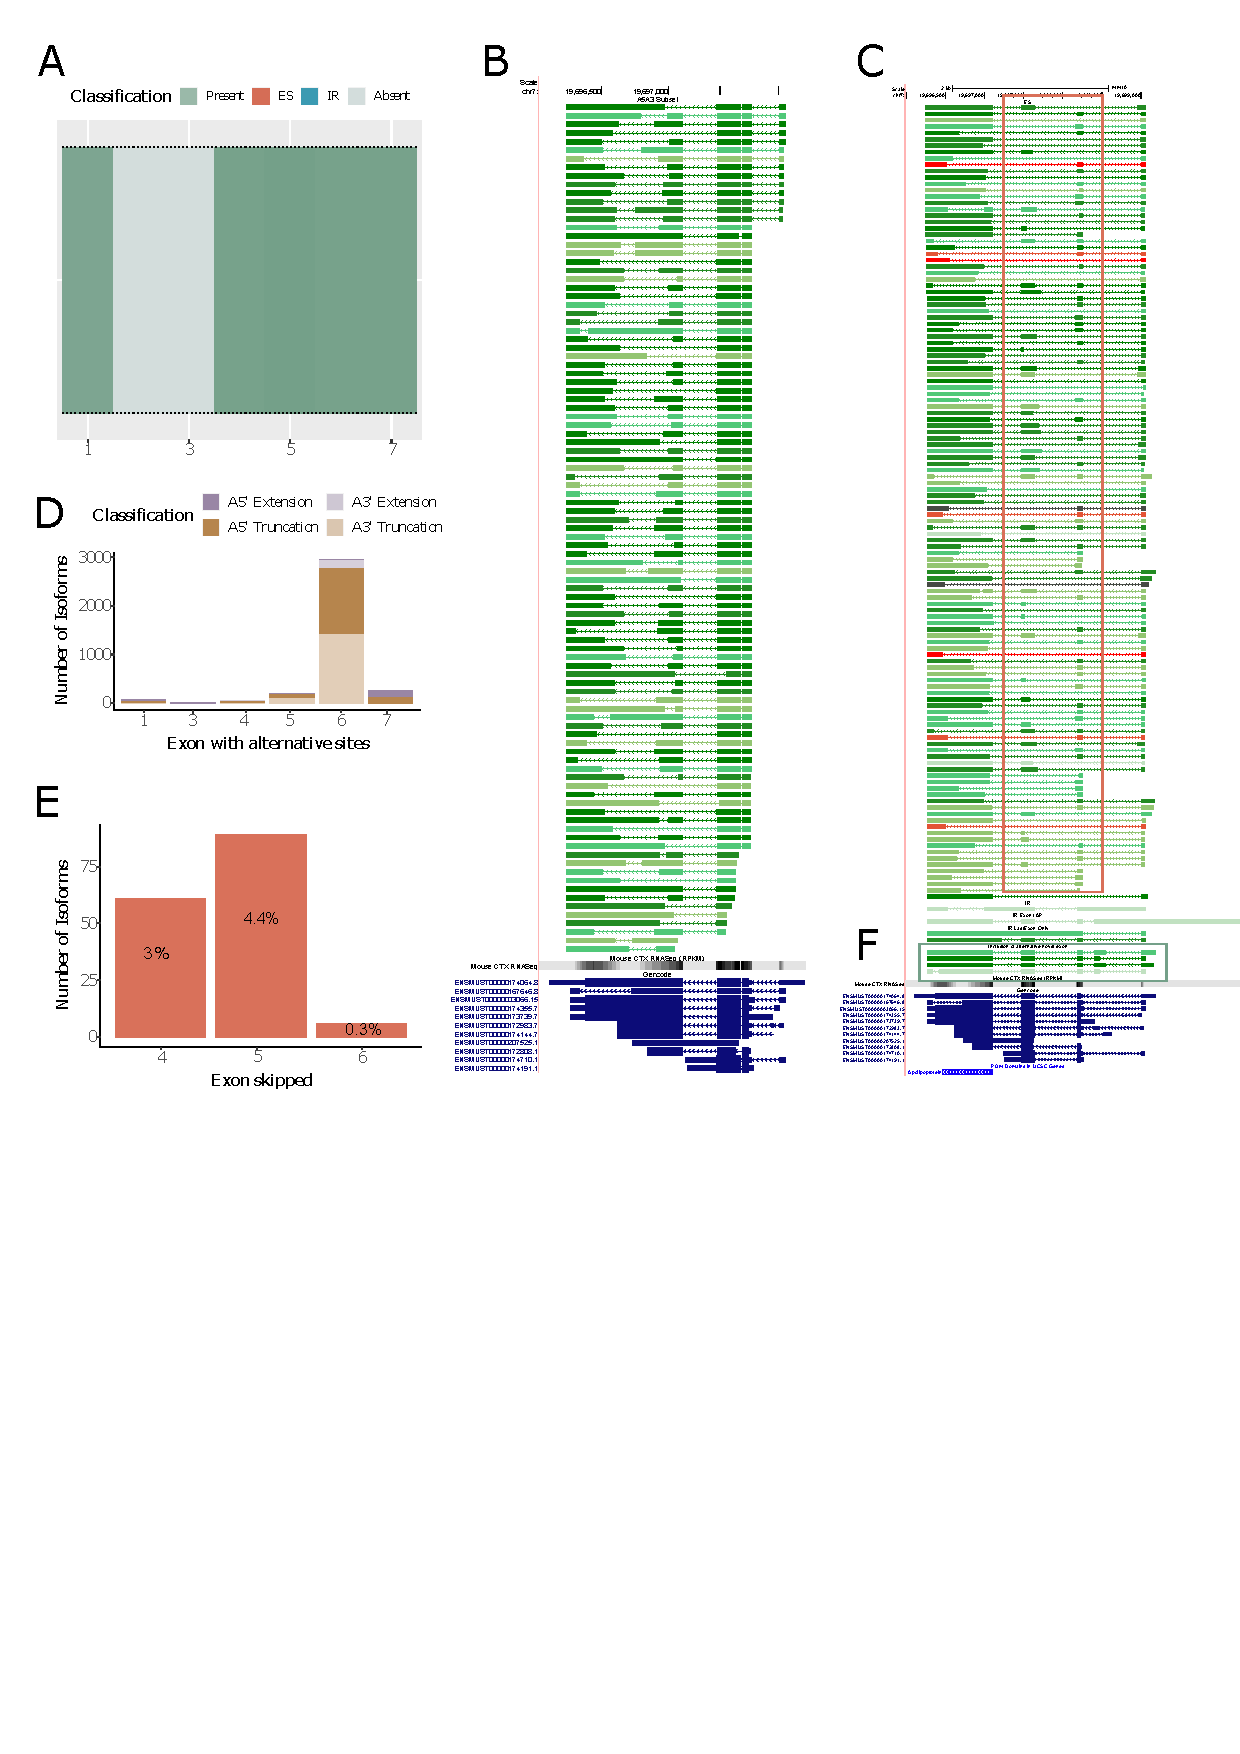
\includegraphics[page=1,trim={0cm 11cm 0 0},scale = 0.85]{Figures/TargetGenes_Annotation_Portrait.pdf}
	\captionsetup{width=0.95\textwidth}
	\caption[Characterisation of the \textit{Apoe} isoform landscape]%
	{\textbf{Characterisation of \textit{Apoe} isoforms in the rTg4510 cortex.} Shown are \textbf{(A)} a cluster dendrogram for an overview of the \textit{Apoe} isoform landscape (exons 2, 3 and 4 are alternative first exons from other known reference isoforms), \textbf{(B)} UCSC genome browser tracks of isoforms annotated to \textit{Ank1} with usage of alternative 5' and 3' splice sites, and \textbf{(C)} exon skipping events (box red), and \textbf{(D)} a bar-plot of the number of isoforms with alternative 5' and 3' splice sites, and \textbf{(E)} exon skipping events.}    
	\label{fig:apoe}
\end{figure}

\newpage
\subsubsection{App}
The amyloid precursor protein gene, \textit{APP}, is well-established in playing a key role in AD pathogenesis. Central to the amyloid cascade hypothesis (described in \cref{aetiologyAD}), \textit{APP} encodes the integral membrane protein that is sequentially cleaved to generate A$\beta$ peptides of varying lengths. Over 50 mutations are identified in \textit{APP} and are known to cause Familial's Alzheimer's Disease\cite{Li2019,D1996,JT1993}. 

Spanning over 224kb on chromosome 16, the mouse \textit{App} gene is characterised with 18 exons and 11 known isoforms. In contrast to the mouse reference annotations and in spite of the relatively few exons associated with \textit{App}, we detected 466 isoforms annotated to \textit{App}. We identified isoforms with varying lengths with less than half spanning the full length of the gene (n = 183, 39.9\%) (\cref{fig:app}\textbf{A}). A number of the shorter isoforms shared similar exonic structure to the two known short isoforms - App-205 (ENSMUST00000227654.1) and App-210 (ENSMUST00000228375.1) (\cref{fig:app}\textbf{H}). However, the majority of the shorter isoforms (n = 428, 91.8\%) were characterised with alternative first exons while preserving the 3'end exonic structure (\cref{fig:app}\textbf{A}), which contained the uncleaved $\beta$-amyloid peptide. 

Despite this variation in isoform length, we observed a consistent splicing pattern with exon skipping (n = 406 isoforms, 87.1\%) enriched in two regions of the gene (\cref{fig:app}\textbf{C}): i) exon 7 (n = 289 isoforms) and exon 8 (n = 304 isoforms) (\cref{fig:app}\textbf{B, F}), which encode the Kunitz protease inhibitor (KPI) domain, ii) exon 14 (n = 392 isoforms) and exon 15 (n = 390 isoforms) (\cref{fig:app}\textbf{B, E}), which were alternative last exons present in only two of the known \textit{App} isoforms (App-208, ENSMUST00000227753.1 and App-209, ENSMUST00000227990.1). With over 60\% of isoforms were characterised with four or more skipping events (n = 291 isoforms, 62.4\% of ES-isoforms) (\cref{fig:app}\textbf{D}), we also detected isoforms with skipping of exon 18 (n = 39 isoforms) and 19 (n = 54 isoforms) (\cref{fig:app}\textbf{B, G}), which encode the uncleaved beta-amyloid peptide. While the majority of known isoforms do not contain exons 7 and 8, most contain the KPI (KPI+) domain, a 57-amino-acid insert with homology to the Kunitz family of serine protease inhibitors. Recent studies investigating differential transcript expression in AD human post-mortem brains have revealed significant downregulation of two isoforms lacking the KPI domain\cite{Marques-Coelho2021}. Noteworthy, increased mRNA and protein expression of KPI(+) transcripts are associated with increased amyloid-beta accumulation\cite{Zhang2011}. 

\newgeometry{left=1cm, right = 1cm, bottom = 2cm, top = 1cm}
\begin{figure}[htp]
	\centering
	\includegraphics[page=2,trim={0 2.2cm 0 0},scale = 0.85]{Figures/TargetGenes_Annotation_Portrait.pdf}
	\captionsetup{width=0.95\textwidth}
	\caption[Characterisation of the \textit{App} isoform landscape]%
	{\textbf{Characterisation of \textit{App} isoforms in the rTg4510 cortex.} Shown are \textbf{(A)} a cluster dendrogram for an overview of the \textit{App} isoform landscape, \textbf{(B)} a UCSC genome browser track of a subset of \textit{App}-associated isoforms with exon skipping (boxed in red), \textbf{(C)} a bar-plot of the number of isoforms with exon skipping, and \textbf{(D)} isoforms with the total number of exons skipped, \textbf{(E)} zoomed-in UCSC genome browser tracks showing skipping of exons 14 and 15, \textbf{(F)} exon 7 encoding the KPI domain, \textbf{G} exons 18 and 19 encoding the uncleaved beta amyloid peptide, and \textbf{(H)} a UCSC genome browser track of the short isoforms that aligned with App-205 (ENSMUST00000227654.1).}    
	\label{fig:app}
\end{figure}
\restoregeometry

\newpage
\subsubsection{Bin1}
\label{ch5: bin1_annotation}
Bridging Integrator 1 gene, \textit{BIN1}, is a well-established AD risk gene with multiple AD-associated SNPs from GWAS studies, and remains second only after \textit{APOE} in genome-wide significance\cite{Kunkle2019}. Although the mechanisms underlying the role of \textit{BIN1} in AD pathogenesis is not fully understood, recent transcriptomic profiling studies on human post-mortem AD brains have revealed differential cell-specific \textit{BIN1} transcript expression associated with tau accumulation and AD-related traits\cite{Taga2020}. 

Spanning over 58kb on chromosome 18, the mouse \textit{Bin1} gene is characterised with 20 unique exon and 6 known isoforms. In our dataset, we detected 368 isoforms annotated to \textit{Bin1} and identified widespread occurrence of exon skipping, particularly within certain regions of the gene (\cref{fig:bin1}\textbf{A}). Drawing parallels to the human-equivalent \textit{BIN1} isoform landscape\cite{Taga2020}, inclusion of exons 14-16, which encode the CLAP domain involved in endocytosis, was highly variable among isoforms (\cref{fig:bin1}\textbf{B,C}) (Exon 14 skipping: 104 isoforms, Exon 15 skipping: 174 isoforms, Exon 16 skipping: 249 isoforms). Strikingly, the most abundant isoform detected in both our Iso-Seq (8,769 Iso-Seq full-length reads) and ONT targeted datasets (40,622 ONT full-length reads) was a novel isoform (PB.3915.2\_TALONT000761829) that shared a similar exonic structure to the known canonical isoform (ENSMUST00000025239.8, which was the second most abundant isoform with 4,120 Iso-Seq full-length reads and 18,451 ONT full-length reads) with the exclusion of exon 15. ORF prediction of this isoform showed that skipping of this exon maintained the reading frame. This region, encoding the CLAP domain, was also notably enriched with occurrence of intron retention events (n = 48 events, 25 isoforms) (\cref{fig:bin1}\textbf{D,E}). In contrast, the first 10 exons, which encode the N-BAR domain involved in membrane curvature, were relatively more conserved in these long isoforms with fewer splicing events. 

Despite the relatively conserved nature of the N-BAR domain, we detected a number of shorter isoforms that were characterised with an alternative first exon and subsequent exclusion of this domain (\cref{fig:bin1}\textbf{F}). Sharing similar exonic structure to Bin1-204 (ENSMUST00000234373.1), some of these isoforms were further characterised with a long alternative first exon that spanned across the CLAP domain. 

\newgeometry{left=1cm, right = 1cm, bottom = 2cm, top = 0.5cm}
\begin{figure}[htp]
	\centering
	\includegraphics[page=3,trim={0 1cm 0 0},scale = 0.85]{Figures/TargetGenes_Annotation_Portrait.pdf}
	\captionsetup{width=0.95\textwidth}
	\caption[Characterisation of the \textit{Bin1} isoform landscape]%
	{\textbf{Characterisation of \textit{Bin1} isoforms in the rTg4510 cortex.} Shown are \textbf{(A)} a cluster dendrogram for an overview of the \textit{Bin1} isoform landscape, \textbf{(B)} a UCSC genome browser track of the subset of \textit{Bin1}-associated with exon skipping (boxed in red), \textbf{(C)} a bar-plot of the number of isoforms with exon skipping, and \textbf{(D)} intron retention events, \textbf{(E)} a zoomed-in UCSC genome browser tracks showing intron retention events spanning across exons 16-17, and \textbf{(F)} a UCSC genome browser track of the short isoforms that aligned with Bin1-204 (ENSMUST00000234373.1) with the alternative long exon boxed in blue.}    
	\label{fig:bin1}
\end{figure}
\restoregeometry

\newpage
\subsubsection{Cd33}
\label{ch5: cd33_annotation}
Sialic acid-binding immunoglobulin-like lectin 3 gene, known as \textit{Cd33}, is implicated in AD by the identification of various AD-associated variants from GWAS studies. Encoding a myeloid-specific transmembrane receptor involved in key cell-signalling pathways, \textit{Cd33} is implicated in cell adhesion, immune cell growth and cytokine release\cite{Griciuc2019}. Notably, the protective \textit{CD33} AD-associated variant has been correlated with decreased levels of A$\beta$ peptides in AD brains as a consequence of enhanced phagocytosis\cite{Bhattacherjee2021}. 

Spanning across 16kb on chromosome 7, the mouse \textit{Cd33} gene is characterised with 9 unique exons and 6 known isoforms. In our dataset, we detected 41 isoforms annotated to \textit{Cd33}, including 5 of the known isoforms (\cref{fig:cd33}). Reflecting the isoform landscape of the mouse reference annotations, the majority of isoforms detected were similarly short, lacked the first two exons and skipped exon 8 (which was only present in one of the known isoforms Cd33-201, ENSMUST00000004728.11) (\cref{fig:cd33}\textbf{A}). ORF predictions showed that skipping of this exon slightly reduced but maintained the reading frame (\cref{fig:cd33_orf}\textbf{A}). In contrast, deeper evaluation revealed that truncation (alternative 3' splice site) of exon 4 shifted the reading frame as a result of generating a stop codon (\cref{fig:cd33_orf}\textbf{A}). Consequently, the reading frame of such isoforms appeared to be driven by a downstream initiator codon in exon 5, resulting in exon 4 exclusion. Notably, exons 4 and 5 encode the two immunoglobulin domains.  

Although the majority of isoforms were relatively short, we detected a few novel isoforms that spanned the length of the gene and incorporated features from different known isoforms. One example included a novel isoform that shared the 5' exonic structure of Cd33-202 (ENSMUST00000039861.6), while simultaneously harbouring the longer 3'UTR only present in Cd33-203 (ENSMUST00000205503.1) (\cref{fig:cd33}\textbf{D}). We further detected two novel isoforms with a novel exon present between exon 1 and exon 2  (66bp, Chr7:43529866-43529932, \cref{fig:cd33_orf}\textbf{B}). ORF predictions showed that inclusion of the novel exon did not alter the reading frame. 

While exon skipping was localised to exon 8, we observed widespread occurrence of intron retention (IR) events across \textit{Cd33}. Over a third of the isoforms detected (n = 14, 34.21\%) contained at least one IR event (\cref{fig:cd33}\textbf{B}), with one isoform containing an IR event that spanned across 4 exons (TALONT001237573, \cref{fig:cd33_orf}\textbf{C}). Deeper characterisation revealed that intron retention primarily occurred around exon 7 (\cref{fig:cd33}\textbf{C}) and extended to the final two exons, exon 8 and exon 9, with varying lengths (\cref{fig:cd33_orf}\textbf{C}). ORF predictions showed that an extended intron retention at exon 7 revealed a stop codon resulting in a shortened reading frame, whereas an intact exon 7 resulted in a slightly longer reading frame.

\newgeometry{left=1cm, right = 1cm, bottom = 2cm, top = 2cm}
\begin{landscape}
	\begin{figure}[htp]
		\centering
		\captionsetup{width=1.3\textwidth}
		\includegraphics[page=4,trim={0 3cm 0 0},scale = 0.85]{Figures/TargetGenes_Annotation_Landscape.pdf}
		\caption[Characterisation of the \textit{Cd33} isoform landscape]%
		{\textbf{Characterisation of \textit{Cd33} isoforms in the rTg4510 cortex.} Shown are \textbf{(A)} a cluster dendrogram for an overview of the \textit{Cd33} isoform landscape, \textbf{(C)} a bar-plot of the number of isoforms with intron retention events, and \textbf{(D)} the number of exons characterised with IR, and \textbf{(D)} a UCSC genome browser track of the detected isoforms that aligned with known \textit{Cd33} isoforms. Intron retention events are further classified as "IR" it occurs at one exon or "IR Match" if it spans across multiple exons.}    
		\label{fig:cd33}
	\end{figure}
\end{landscape}

\begin{landscape}
	\begin{figure}[htp]
		\centering
		\captionsetup{width=1.3\textwidth}
		\includegraphics[page=5,trim={0 3.5cm 0 0},scale = 0.85]{Figures/TargetGenes_Annotation_Landscape.pdf}
		\caption[Characterisation of the \textit{Cd33} splicing landscape]%
		{\textbf{Characterisation of \textit{Cd33} splicing events in the rTg4510 cortex.} Shown are UCSC genome browser tracks of \textbf{(A)} \textit{Cd33} isoforms with exon skipping and the respective predicted open reading frame - the exon truncation and the shift in reading frame are denoted by the pink box and pink arrow, respectively - \textbf{(B)} two novel long isoforms with presence of a novel exon located between exon 1 and exon 2 (boxed), and \textbf{(C)} isoforms characterised with intron retention (IR) events - the isoform with IR spanning across 4 exons is highlighted in yellow.}    
		\label{fig:cd33_orf}
	\end{figure}
\end{landscape}
\restoregeometry 

\newpage
\subsubsection{Clu}
The clusterin gene, \textit{CLU}, is strongly associated with late-onset AD along with \textit{APOE} and \textit{BIN1}\cite{Lambert2013}. Encoding a glycoprotein with chaperone function, clusterin has been implicated in various pathways including immune regulation, lipid homeostasis and apoptosis\cite{Foster2019}. While the role of clusterin in AD pathology is not fully understood, recent studies have reported upregulation of clusterin in AD brains with a suggestive role in altering A$\beta$ aggregation\cite{Jackson2019}. 

Spanning over 13kb on chromosome 14, the mouse \textit{Clu} gene is characterised with 14 unique exons and 9 known isoforms. In our dataset, we identified 733 isoforms annotated to \textit{Clu} in the mouse rTg4510 cortex. Although the isoform diversity in the mouse reference genome annotations was predominantly driven by alternative first exons (n = 6 alternative first exons across 9 known isoforms), the majority of isoforms detected (n = 402, 55\%) were derived from the first upstream exon from Clu-201 (ENSMUST00000022616.13) and spanned the full-length of the clusterin domain (\cref{fig:clu}\textbf{A,B}). Notably, we identified a handful of novel isoforms with novel alternative first exons (\cref{fig:clu}\textbf{B}), highlighting the extensive usage of alternative first exons as a transcriptional mechanism of \textit{Clu} expression. ORF predictions, however, showed that translation was initiated at the start site located in exon 7, bypassing all the alternative first exons. Drawing parallels to the human \textit{CLU} gene\cite{Foster2019}, alternative start codons were also identified in the upstream exons, though their functional importance are unknown. We further identified the N-terminal endoplasmic reticulum (ER)-signal peptide with a cleavage site (position 21-22) within exon 7, allowing generation of secreted CLU\cite{Foster2019}.   

Deeper characterisation of our dataset revealed that \textit{Clu} isoform diversity was primarily driven by extensive usage of alternative 5' and 3' splice sites, and occurrence of exon skipping and intron retention events localised to certain regions of the gene (\cref{fig:clu}\textbf{A}), notably: skipping of exon 9 (n = 143 isoforms  19.5\%), exon 10 (n = 129 isoforms, 17.6\%) and exon 11 (n = 165 isoforms, 22.5\%) (\cref{fig:clu}\textbf{C,D}). ORF predictions showed that skipping of these exons reduced but maintained the reading frame. Conversely, intron retention events (n = 217 events) predominantly occurred at the 5'-end of the gene with intron retention spanning across exons 6, 7 and 8 (\cref{fig:clu}\textbf{E}). Noteworthy, exon 6 refers to an alternative first exon from Clu-206 (ENSMUST00000144619.1). ORF prediction of these isoforms showed that there was a shift in open reading frame with initiation of translation at exon 10. On the other hand, the effect of IR spanning across exons 7 and 8 on the reading frame appeared to be dictated by the upstream first exon: usage of the first exon from the canonical isoform, Clu-201 (ENSMUST00000022616.13), resulted in a truncated protein from translation at exon 10, whereas usage of the first exon from Clu-207 (ENSMUST00000146990.1) resulted in a truncated protein destined for nonsense-mediated decay (\cref{fig:clu}\textbf{F}). 



\newgeometry{left=1cm, right = 1cm, bottom = 2cm, top = 2cm}
\begin{landscape}
	\begin{figure}[htp]
		\centering
		\captionsetup{width=1.3\textwidth}
		\includegraphics[page=6,trim={0 1.5cm 0 0},scale = 0.85]{Figures/TargetGenes_Annotation_Landscape.pdf}
		\caption[Characterisation of the \textit{Clu} isoform landscape]%
		{\textbf{Characterisation of \textit{Clu} isoforms in the rTg4510 cortex.} Shown are \textbf{(A)} a cluster dendrogram for an overview of the \textit{Clu} isoform landscape, \textbf{(B)} UCSC genome browser tracks of isoforms annotated to \textit{Clu} that shared exonic structure with the long \textit{Clu} isoform (Clu-201), and \textbf{(C)} isoforms characterised with exon skipping events, \textbf{(D)} bar plots of the number of isoforms with exon skipping, \textbf{(E)} number of isoforms with intron retention events, and \textbf{(G)} a UCSC genome browser tracks of two \textit{Clu} isoforms with intron retention spanning across exon 7 and 8, resulting in two different open reading frames.}    
		\label{fig:clu}
	\end{figure}
\end{landscape}
\restoregeometry



\newpage
\subsubsection{Fus}
The Fused in sarcoma gene, \textit{Fus}, is a well-established causative gene for a number of neurodegenerative diseases, including ALS and FTD. Encoding the subunit of the heterogeneous nuclear ribonucleoprotein complex, a multi-functional DNA/RNA-binding protein,  \textit{Fus} is implicated in key cellular processes including transcriptional regulation, DNA repair and alternative splicing\cite{Shelkovnikova2014}. Increasing evidence suggests that aggregates of the FUS proteins followed by formation of intracellular inclusion bodies are key initiator events in disease onset and pathology\cite{Shelkovnikova2014}. Notably, \textit{Fus} neuronal aggregates has become the characteristic pathological hallmark for the subset of sporadic FTD cases that lack the more established inclusion markers of TDP-43 and tau\cite{Seelaar2010}.

Spanning across 18kb on chromosome 7, the mouse \textit{Fus} gene is a complex gene characterised with multiple known isoforms of varying lengths. However, in contrast to the \textit{Fus} isoform landscape in the mouse reference genome annotations, the \textit{Fus} splicing pattern in our dataset was relatively simpler (\cref{fig:fus}\textbf{A}): a quarter (n = 53, 25.7\%) of the isoforms detected (n = 236 isoforms) largely shared the exonic structure of the long known isoform that spanned the full-length of the gene, differing only by minor variations (<10bp, "wobble") at the splice site (\cref{fig:fus}\textbf{B}). 

Despite this relatively simple isoform landscape, we detected widespread occurrence of exon skipping (\cref{fig:fus}\textbf{C,D}) and intron retention events (\cref{fig:fus}\textbf{E,F}) that were not existing in the reference mouse genome. Over 40\% of isoforms detected (n = 103, 43.6\%) were characterised with at least one exon skipping event, with exon 8 skipped in half of the these isoforms (n = 50 isoforms, n = 48.5\% of isoforms with exon skipping, \cref{fig:fus}\textbf{D}). Intron retention events were further localised to this region of the \textit{Fus} gene: 17 isoforms were identified with intron retention events spanning across exons 6, 7 and 8. While such IR events were also present in the known isoforms - Fus-206 (ENSMUST00000128851.7) - the majority of the detected IR events spanning across this region belonged to the first exon rather than an internal exon (\cref{fig:fus}\textbf{F}). Consequently, the isoforms detected contained an alternative first exon. Finally, we also detected a number of intron retention events at the 3'end of the \textit{Fus} gene between exons 12 and 14 (\cref{fig:fus}\textbf{F}), which encode the zinc-finger-containing RGG-Znf-RGG domain (zF-RanBP) essential for RNA recognition and binding\cite{Wang2015c}. 

\newgeometry{left=1cm, right = 1cm, bottom = 2cm, top = 1cm}
\begin{figure}[htp]
	\centering
	\includegraphics[page=4,trim={0 4cm 0 0},scale = 0.85]{Figures/TargetGenes_Annotation_Portrait.pdf}
	\captionsetup{width=0.95\textwidth}
	\caption[Characterisation of the \textit{Fus} isoform landscape]%
	{\textbf{Characterisation of \textit{Fus} isoforms in the rTg4510 cortex.} Shown are \textbf{(A)} a cluster dendrogram for an overview of the \textit{Fus} isoform landscape, \textbf{(B)} UCSC genome browser tracks of the subset of isoforms that spanned the full-length of the \textit{Fus} gene with minor splice site variation, \textbf{(C)} isoforms characterised with exon skipping events, \textbf{(D)} bar-plots of the number of isoforms with exon skipping and \textbf{(E)} intron retention events, and \textbf{(F)} a zoomed-in UCSC genome browser tracks of isoforms with intron retention spanning across exons 6, 7 and 8 and between exons 12 and 14 (boxed in blue).}    
	\label{fig:fus}
\end{figure}
\restoregeometry

\newpage
\subsubsection{Fyn}
The non-receptor tyrosine kinase, FYN, is implicated in AD pathogenesis as a consequence of its interactions with tau\cite{Bhaskar2010}. Overexpression of FYN, which is known to directly phosphorylate tau\cite{Bhaskar2010}, was shown to accelerate synaptic and cognitive impairments in a mouse model of AD\cite{Chin2005}. Recent studies have further identified an isoform-specific role of \textit{FYN} in modulating neurofibrillary degeneration with evidence of isoform switching in the AD neocortex\cite{Lee2016b}. 

Spanning over 196 kb on chromosome 10, the mouse \textit{Fyn} gene is associated with 20 unique exons and 9 known isoforms that primarily differ by an alternative first exon. Detecting 50 isoforms annotated to \textit{Fyn}, we found these first exons (exons 1 - 6) were mutually exclusive with isoforms containing either exon 2, exon 3 or exon 4 (\cref{fig:fyn}\textbf{A}). Conversely, exon 1, 5 and exon 6 - the other three alternative first exons - were not solely featured in any of the isoforms except in an intron retention event (\cref{fig:fyn}\textbf{A}). Notably, we detected a number of novel isoforms with novel alternative first exons located at three distinct regions (\cref{fig:fyn}\textbf{C}): i) between exons 2 and 3, ii) exons 4 - 5 and ii) at exon 8. Despite the widespread usage of alternative first exons and promoter, ORF prediction showed that inclusion of these novel first exons did not alter the reading frame, which was still predicted to start from exon 7.  

In contrast to the complexity at the 5'end of the \textit{Fyn} gene, which does not encode for any protein domains, the exonic structure downstream of exon 7 was relatively conserved (\cref{fig:fyn}\textbf{A}). Exons that encode the SH3 domain (exons 7 to 12), which is known to interact with tau, were present in all the isoforms detected (\cref{fig:fyn}). Notably, exons 13 and 14, which encode the protein kinase domain, were found to be mutually exclusive (\cref{fig:fyn}\textbf{A,B,C}); the majority of detected isoforms contained exon 13 (n = 36) and skipped exon 14 (\cref{fig:fyn}). Finally, we noted a complete exclusion of exon 16, which was only present in Fyn-203 as an alternative first exon (\cref{fig:fyn}\textbf{A,C}). 

\newgeometry{left=1cm, right = 0.7cm, bottom = 2cm, top = 2cm}
\begin{landscape}
	\begin{figure}[htp]
		\centering
		\captionsetup{width=1.3\textwidth}
		\includegraphics[page=7,trim={0 1cm 0 0},scale = 0.85]{Figures/TargetGenes_Annotation_Landscape.pdf}
		\caption[Characterisation of the \textit{Fyn} isoform landscape]%
		{\textbf{Characterisation of \textit{Fyn} isoforms in the rTg4510 cortex.} Shown are \textbf{(A)} a cluster dendrogram for an overview of the \textit{Fyn} isoform landscape, \textbf{(B)} a bar-plot of the number of isoforms with exon skipping, and \textbf{(C)} a UCSC genome browser track of isoforms characterised with exon skipping (boxed red) events and presence of novel exons (boxed green).}    
		\label{fig:fyn}
	\end{figure}
\end{landscape}
\restoregeometry

\newpage
\subsubsection{Mapt}
The microtubule-associated protein tau gene, \textit{MAPT}, is a well-established gene in AD pathogenesis. Central to the tau hypothesis (described in \cref{aetiologyAD}), \textit{MAPT} encodes the tau protein essential for microtubule stability and maintenance. Tau mutations associated with frontotemporal dementia and parkinsonism (FTDP), which result in altered ratio of tau isoforms, are known to induce tau phosphorylation and aggregation\cite{Bowles2022}. While no causative \textit{MAPT} mutations have been identified in AD, tau aggregation and subsequent formation of neurofibrillary tangles are one of the key hallmarks of AD pathology (described in \cref{ch1: ad_pathology}). 

Spanning over 100kb on chromosome 11, the mouse \textit{Mapt} gene is characterised with 16 unique exons and 12 known isoforms. In our dataset, we detected 140 isoforms annotated to \textit{Mapt}, including 7 of the known isoforms. Deeper examination of the \textit{Mapt} isoform landscape revealed consistent exon skipping events that alternated across the gene (\cref{fig:mapt}\textbf{A,B,C}); exons 4, 6, 8, 10 and 13 were typically skipped, whereas exons 2, 7, 11, 12 and 14 were typically included. The majority of isoforms were characterised with at least one exon skipping event (n = 115, 82.1\%) with most isoforms skipping 3 or more exons (n = 98, 70\%). ORF prediction showed that all these exon skipping events reduced but maintained the reading frame. 

Finally, using Iso-Seq and ONT nanopore sequencing, we detected some significantly shorter isoforms that were distinguished by the presence of a alternative first exon characterised with intron retention (\cref{fig:mapt}\textbf{F}). These broadly appeared between exons 9 and 11, which encode the tubulin-binding repeat domain. ORF predictions of these isoforms revealed that intron retention that significantly spanned across exons 7, 8 and 9 generated a truncated product destined for nonsense-mediated decay, whereas intron retention events that spanned across exons 10 and 11 maintained the reading frame (\cref{fig:mapt}\textbf{D}). 


\newgeometry{left=1cm, right = 1cm, bottom = 2cm, top = 1cm}
\begin{figure}[htp]
	\centering
	\includegraphics[page=5,trim={0 10cm 0 0},scale = 0.85]{Figures/TargetGenes_Annotation_Portrait.pdf}
	\captionsetup{width=0.95\textwidth}
	\caption[Characterisation of \textit{Mapt} isoforms in the rTg4510 cortex]%
	{\textbf{Characterisation of \textit{Mapt} isoforms in the rTg4510 cortex.} Shown are \textbf{(A)} a cluster dendrogram for an overview of the \textit{Mapt} isoform landscape, \textbf{(B)} a UCSC genome browser track of a subset of isoforms with exon skipping (boxed in red), \textbf{(C)} a bar-plot of the number of isoforms with exon skipping, and \textbf{(D)} a zoomed-in track of the shorter isoforms with an alternative first exon characterised with intron retention. The isoforms with intron retention spanning across exons 7 and 9 generated a truncated peptide destined for nonsense-mediated decay (highlighted in yellow), whereas the isoforms with intron retention spanning across exons 10 and 11 maintained the reading frame (highlighted orange).}    
	\label{fig:mapt}
\end{figure}
\restoregeometry

\newpage
\subsubsection{Picalm}
The phosphatidylinositol-binding clathrin assembly protein gene, \textit{PICALM}, is another reproducible AD-risk gene identified by GWAS. Emerging evidence suggest that \textit{PICALM}, which encodes an adaptor protein involved in clathrin-mediated endocytosis,  mediates AD-risk by modulating production, trafficking and clearance of A$\beta$ peptide\cite{Ando2016}. Recent studies further showed that increased expression of \textit{PICALM} rescued endocytic effects associated with \textit{APOE}4\cite{Narayan2020}.

Spanning over 83kb on chromosome 7, the mouse \textit{Picalm} gene is associated with 22 unique exons and 15 known isoforms. In our dataset, we detected 144 isoforms annotated to \textit{Picalm}, including all the known isoforms bar the non-coding isoform Picalm-208 (ENSMUST00000207949.1). Approximately a fifth of the isoforms detected (n = 31, 21.5\%) spanned the full-length of the \textit{Picalm} gene, while the remaining isoforms were significantly shorter and characterised with an alternative first exon (\cref{fig:picalm}\textbf{A,D}). Notably, we identified a novel isoform (PB.7635.2\_TALONT001254093) that contained a novel exon 59kb upstream of exon 1 (\cref{fig:picalm}\textbf{F}). ORF prediction of this isoform, which was detected using both PacBio Iso-Seq and ONT nanopore sequencing, predicted a reading frame initiated from this novel first exon.  

Although the exonic structure was broadly conserved across the isoforms (\cref{fig:picalm}\textbf{B,C}), we observed consistent exon skipping of exons 13, 18, and 21 (\cref{fig:picalm}\textbf{C,E}), which do not encode the ANTH or ENTH protein domains; the ANTH domain is a membrane binding domain implicated in the formation of clathrin-coated pits, while the ENTH domain mediates membrane curvature and subsequent endocytosis. ORF predictions showed that skipping of such exons shortened but maintained the reading frame. 

%However, the vast majority of coding isoforms were predicted to undergo nonsense mediated decay (n = 115, 98.3\%) including the known reference isoforms. Further examination revealed that while the reading frame varied at the 5'end from alternative first exon usage, all the reading frames 

\newgeometry{left=1cm, right = 1cm, bottom = 2cm, top = 2cm}
\begin{landscape}
	\begin{figure}[htp]
		\centering
		\captionsetup{width=1.3\textwidth}
		\includegraphics[page=8,trim={0 1cm 0 0},scale = 0.8]{Figures/TargetGenes_Annotation_Landscape.pdf}
		\caption[Characterisation of the \textit{Picalm} isoform landscape]%
		{\textbf{Characterisation of \textit{Picalm} isoforms in the rTg4510 cortex.} Shown are \textbf{(A)} a cluster dendrogram for an overview of the \textit{Picalm} isoform landscape, \textbf{(B)} UCSC genome browser tracks of the isoforms that aligned to the reference isoforms, \textbf{(D)} isoforms with exon skipping events (highlighted in red), \textbf{(D)} bar-plots of the number of isoforms with alternative first exons, \textbf{(E)} number of isoforms with exon skipping, and \textbf{(F)} a UCSC genome browser track of the novel isoform containing a novel exon upstream of the gene.}    
		\label{fig:picalm}
	\end{figure}
\end{landscape}
\restoregeometry

\newpage
\subsubsection{Ptk2b}
Compelling evidence implicates the Protein Tyrosine Kinase 2 Beta gene, \textit{PTK2B}, in AD pathology with consistent identification of genetic variants associated with AD risk\cite{Lambert2013,Kunkle2019}. Encoding a protein tyrosine kinase involved in key signalling pathways, Pyk2, \textit{Ptk2b} is involved in synaptic plasticity and activity. Of note, increased \textit{Ptk2b} expression in a mouse model corrected deficits in synaptic proteins and improved the behaviour phenotype of transgenic mice\cite{Giralt2018}. A recent study further revealed a direct association of AD-associated \textit{Ptk2b} genetic variant with altered splicing\cite{Raj2018}, though the mechanism underlying the role of \textit{Pkt2b} in AD pathology remains unclear.

Spanning over 127kb on chromosome 14, the mouse \textit{Pt2kb} gene is associated with 31 unique exons and 8 known isoforms. Drawing parallels to the human-equivalent \textit{PTK2B}, the mouse \textit{Pt2kb} gene is similarly characterised with a tyrosine kinase domain flanked by a N-terminal FERM domain and a C-terminal FAT (focal adhesion targeting) domain\cite{DePins2021}. In our dataset, we detected 563 isoforms annotated to \textit{Ptk2b}. Deeper examination of \textit{Pt2kb}-annotated isoforms revealed isoforms with varying lengths, containing exons that encode the kinase and FAT domain and not the N-terminal FERM domain (\cref{fig:ptk2b}\textbf{A}). Previous studies have similarly identified human-equivalent isoforms missing the FERM and kinase domains\cite{DePins2021}, and these isoforms were predicted to be transcribed from an alternative promoter as an endogenous regulator of Pyk2 activity\cite{DePins2021}.

Finally, we noticed that while the exonic structure was largely conserved across the gene (\cref{fig:ptk2b}\textbf{B}), we detected high occurrence of exon skipping events localised to exon 27 (n = 296, 52.5\%) (\cref{fig:ptk2b}\textbf{C,D}). ORF predictions showed that skipping of this 24bp exon, which was present across all the known isoforms (i.e. "constitutive"), shortened but maintained the reading frame. We also detected a few isoforms with intron retention events (n = 6, 1.1\%). Examination of these IR events found them to be localised to the first exon of the shorter isoforms  (\cref{fig:ptk2b}\textbf{E}), which shared a similar exonic structure to Ptk2b-205 (ENSMUST00000136216.7) in spanning across the 3'-end and containing exons encoding the FAT domain. ORF predictions revealed that intron retention events spanning across exons 29 and 30 resulted in a reading frame shift with a truncated isoform predicted for nonsense-mediated decay (\cref{fig:ptk2b}\textbf{E}). Conversely, intron retention events that spanned across exons 25 to 28, thereby keeping exons 29 and 30 intact, maintained the reading frame with translation of a 125-amino-acid-peptide containing the FAT domain (\cref{fig:ptk2b}\textbf{E}). 


\newgeometry{left=1cm, right = 1cm, bottom = 2cm, top = 1cm}
\begin{figure}[htp]
	\centering
	\includegraphics[page=6,trim={0 2cm 0 0},scale = 0.85]{Figures/TargetGenes_Annotation_Portrait.pdf}
	\captionsetup{width=0.95\textwidth}
	\caption[Characterisation of the \textit{Ptk2b} isoform landscape]%
	{\textbf{Characterisation of \textit{Ptk2b} isoforms in the rTg4510 cortex.} Shown are \textbf{(A)} a cluster dendrogram for an overview of the \textit{Ptk2b} isoform landscape, \textbf{(B)} a UCSC genome browser track of a subset of isoforms that shared a similar internal exonic structure but varied at the 5'end, \textbf{(C)} bar-plots of the number of isoforms with exon skipping, \textbf{(D)} zoomed-in tracks of isoforms with skipping of exon 27 and of \textbf{(F)} isoforms with intron retention events. Isoforms characterised with an intron retention event spanning across exons 29 and 30 were predicted for NMD (boxed yellow, isoforms not predicted for NMD are boxed in blue)}    
	\label{fig:ptk2b}
\end{figure}
\restoregeometry

\newpage
\subsubsection{Rhbdf2}
Aside from \textit{Ank1} (described in \cref{ch6: ank1}), AD EWAS studies have consistently identified a differentially-methylated region residing in \textit{RHBDF2}, a gene that encodes a rhomboid serine protease essential for  TNF$\alpha$ secretion. The role of \textit{RHBDF2} in AD pathogenies, however, remain poorly understood.   

Spanning across 29kb on chromosome 11 with known 19 unique exons, the mouse \textit{Rhbdf2} gene is the second least expressed gene from our panel of AD-associated target genes. In our dataset, we detected five isoforms, including the canonical isoform, Rhbdf2-202 (ENSMUST00000103029.9), and 2 exon skipping events (\cref{fig:rhbdf2}\textbf{A,B}): exon 3 and exon 18, the latter which encodes the rhomboid domain. While \textit{Rhbdf2} exhibited the least complex splicing pattern, ORF predictions of these isoforms revealed reading frame predictions of varying lengths (\cref{fig:rhbdf2}\textbf{B}): i) the known canonical isoform appeared to be translated from an alternative start codon present in exon 3, ii) skipping of exon 3 was associated with a reading frame initiated at exon 5, iii) skipping of exon 18 retained the reading frame from exon 3 but reduced the frame at the 3'-end, and iv) a 5bp-deletion at exon 7 (\cref{fig:rhbdf2}\textbf{C}), which encodes the protease domain, shifted the reading frame and subsequently resulted in usage of an alternative start codon at exon 7 rather than exon 3.  


\newgeometry{left=2cm, right = 2cm, bottom = 2cm, top = 2cm}
\begin{landscape}
	\begin{figure}[htp]
		\centering
		\includegraphics[page=9,trim={0 5cm 0 0},scale = 0.85]{Figures/TargetGenes_Annotation_Landscape.pdf}
		\captionsetup{width=1.3\textwidth}
		\caption[Characterisation of the \textit{Rbhdf2} isoform landscape]%
		{\textbf{Characterisation of \textit{Rhbdf2} isoforms in the rTg4510 cortex.} Shown are \textbf{(A)} a UCSC genome browser track of isoforms annotated to \textit{Rhbdf2}, \textbf{(B)} cluster dendrogram for an overview of the \textit{Rhbdf2} isoform landscape, and \textbf{(C)} a zoomed-in track showing the 5bp deletion at exon 7 which resulted in a reading frame shift and the subsequent usage of the downstream start codon at exon 7.}   
		\label{fig:rhbdf2}
	\end{figure}
\end{landscape}
\restoregeometry

\newpage
\subsubsection{Snca}
Aggregates of the α-synuclein protein, encoded by the \textit{SNCA} gene, are one of the defining hallmarks for a number of neurodegenerative diseases, collectively known as synucleinopathies. Notably, up to 50\% of AD patients are presented with co-morbid $\alpha$Syn pathology. While the precise mechanisms driving synucleinopathies pathogenesis are yet to be determined, there is increasing evidence for the role of altered \textit{SNCA} splicing as a key mechanism for disease development\cite{Beyer2012, Beyer2006}. Of note, recent studies have shown that skipping of exon 6 result in a truncated SNCA protein that exhibit increased propensity to aggregate\cite{Beyer2012, Beyer2006}. 

Spanning across 98kb on chromosome 6, the mouse \textit{Snca} gene is characterised with 8 unique exons and 4 known isoforms. Despite having relatively few exons, \textit{Snca} was the third most "isoformic" gene in our dataset with 622 isoforms. In line with findings from studying human \textit{SNCA} gene\cite{Tseng2019}, the mouse-equivalent full-length \textit{Snca} isoform (Snca-201, ENSMUST00000114268.4), was the most abundant transcript sequenced using Iso-Seq (15,469 Iso-Seq full-length reads) and nanopore sequencing (283,239 ONT full-length reads), making up ~60\% of the total \textit{Snca} mRNA transcripts. 

Comprehensive characterisation revealed widespread usage of alternative splicing events, including exon skipping (\cref{fig:snca}\textbf{A}), and alternative 5' and 3' splice sites (\cref{fig:snca}\textbf{B}). Over 75\% of isoforms (n  = 483, 77.7\%) were identified with at least one exon skipping event. Exon 4 and exon 5, which partially encode the Synuclein domain, were skipped the most (exon 4: n = 249 isoforms; exon 5: n = 206 isoforms) (\cref{fig:snca}\textbf{C,D}), despite being present in all the known isoforms (i.e constitutive). Extensive usage of alternative 5' and 3' sites, particularly A5' truncation, was also observed across the gene with the exception of exon 4 (\cref{fig:snca}\textbf{E}). Strikingly, approximately two-thirds of isoforms detected were either non protein-coding (n = 391, 62.8\%) or did not contain a reading frame (n = 11, 1.7\%) (\cref{fig:snca}\textbf{A,B}), a likely consequence of widespread usage of alternative splice sites combined with exon skipping. 

\newgeometry{left=1cm, right = 1cm, bottom = 2cm, top = 1cm}
\begin{figure}[htp]
	\centering
	\includegraphics[page=7,trim={0 10cm 0 0},scale = 0.85]{Figures/TargetGenes_Annotation_Portrait.pdf}
	\captionsetup{width=0.95\textwidth}
	\caption[Characterisation of the \textit{Snca} isoform landscape]%
	{\textbf{Characterisation of \textit{Snca} isoforms in the rTg4510 cortex.} Shown are \textbf{(A)} a cluster dendrogram for an overview of the \textit{Snca} isoform landscape, \textbf{(B)} UCSC genome browser tracks of the subset of isoforms with alternative 5' and 3' splice sites, and \textbf{(C)} subset of isoforms characterised with exon skipping events, particularly skipping of exons 4 and 5 (boxed in red). Isoforms are coloured by protein-coding potential (green for protein-coding and red for non protein-coding) and shaded by abundance. \textbf{(D)} Bar-plots of the number isoforms with exon skipping, and \textbf{(E)} the number of isoforms with alternative 5' and 3' splice sites.}    
	\label{fig:snca}
\end{figure}
\restoregeometry


\newpage
\subsubsection{Sorl1}
Genetic variation annotated to the sortilin-related receptor gene, \textit{SORL1}, has been repeatedly identified as associated with AD risk\cite{Fernandez2016}. Encoding an endocytic sorting receptor, \textit{SORL1} is involved in trafficking of APP and regulation of A$\beta$ production\cite{Knupp2020}. Of note, recent studies have found that deletion of \textit{SORL1} in hiPSCs (human induced pluripotent stem cells) resulted in cell-type specific endosome enlargement with altered APP localisation\cite{Knupp2020}. Studies on post-mortem AD brain tissues have further revealed altered splicing of \textit{SORL1} with decreased expression of the full-length SORL1 isoform, but consistent expression of the isoform lacking exon 2\cite{Grear2009}.  

Spanning over 160kb on chromosome 9, the mouse \textit{Sorl1} gene is characterised with 49 unique exons and 4 known isoforms. This was in significant contrast to our dataset where we detected 113 isoforms annotated to \textit{Sorl1}. Deeper examination of these isoforms, however, revealed that the majority largely shared the same internal exonic structure with few occurrences of exon skipping and intron retention events (\cref{fig:sorl1}\textbf{A, F}). In contrast, over 75\% (n = 88, 77.9\%) of the isoforms were characterised with an alternative first exon (\cref{fig:sorl1}\textbf{C}), and can be broadly classified into three distinct groups by their alternative last exons: i) exon 37, ii) exon 38 (\cref{fig:sorl1}\textbf{D}) and iii) exon 41 (\cref{fig:sorl1}\textbf{E}). While the alternative last exons of such isoforms were in perfect alignment with one another (\cref{fig:sorl1}\textbf{D,E}), they did not fully match the exon of interest, resulting in extensive variation of exons 37, 38 and 41 (\cref{fig:sorl1}\textbf{B}). Notably, exons 37 and 38 encode the Fibronectin type III (fn3) domain, where most of the rare AD-associated variants were found located \cite{Verheijen2016}. 

\textit{Sorl1} isoform variation in our dataset was thus driven by usage of alternative promoter and termination, generating isoforms of varying lengths that either contained the C-terminus Vps10-domain that binds to neurotrophic factors or the N-terminus fn3 domain. ORF prediction of these isoforms show a shortened, but otherwise intact reading frame with no prediction for nonsense-mediated decay. 

\newgeometry{left=1cm, right = 1cm, bottom = 2cm, top = 2cm}
\begin{landscape}
	\begin{figure}[htp]
		\centering
		\captionsetup{width=1.3\textwidth}
		\includegraphics[page=10,trim={0 0.5cm 0 0},scale = 0.8]{Figures/TargetGenes_Annotation_Landscape.pdf}
		\caption[Characterisation of the \textit{Sorl1} isoform landscape]%
		{\textbf{Characterisation of \textit{Sorl1} isoforms in the rTg4510 cortex.} Shown are \textbf{(A)} a cluster dendrogram for an overview of the \textit{Sorl1} isoform landscape, \textbf{(B)} a bar-plot of the number of isoforms with alternative splice sites, \textbf{(C)} a UCSC genome browser track of the isoforms that shared an identical internal exonic structure but contained an alternative first exon, \textbf{(D)} zoomed-in figure of these isoforms with alternative first exon overlapping exon 41, \textbf{(E)} isoforms with alternative first exon overlapping exon 38, and \textbf{(F)} a UCSC genome browser track displaying isoforms with exon skipping (boxed red) and intron retention (boxed blue) events.}    
		\label{fig:sorl1}
	\end{figure}
\end{landscape}
\restoregeometry

\newpage
\subsubsection{Tardbp}
Aggregates of the transactive response DNA binding protein (TDP-43), encoded by \textit{TARDBP}, has long been established as a hallmark for ALS and Frontotemporal lobar degeneration (FTLD)\cite{Meneses2021}. Notably, deposition of TDP-43 has been associated with the development of severe AD pathology with up to 60\% of AD patients also characterised by TDP-43 pathology \cite{Brouwers2010}. Furthermore, inheritance of APOE4 is associated with increased frequency of TDP-43 pathology, further implicating the role of TDP-43 in AD pathology\cite{Meneses2021}. 

Spanning over 14.6kb on chromosome 4, the mouse \textit{Tardbp} gene is characterised with 10 unique exons and 30 known isoforms. Despite only containing 10 exons, \textit{Tardbp} is one of the most complex gene from our panel of AD-associated target genes; multiple isoforms are characterised with multiple exon overlap across the 3'end of the gene. Detecting 127 isoforms annotated to \textit{Tardbp} in our dataset, we observe a similarly complex isoform landscape capturing the full complement of known non-coding and coding isoforms (\cref{fig:tardbp}\textbf{A,B}). Supplementing the complexity of the 3'end of \textit{Tardbp} gene, we further observed an enrichment of intron retention (IR) events between exons 6, 7 and 8 (\cref{fig:tardbp}\textbf{B,D}). Deeper examination of IR events revealed them to belong to the final exon of some of the shorter detected isoforms (\cref{fig:tardbp}\textbf{C}), resulting in the generation of a novel alternative last exon (\cref{fig:tardbp}\textbf{F}). ORF prediction of these IR-associated isoforms, which were further characterised with alternative 5' and 3' splice sites of the upstream exons (\cref{fig:tardbp}\textbf{E}), revealed a truncated reading frame with such isoforms predicted for nonsense-mediated decay. 


\newgeometry{left=1cm, right = 1cm, bottom = 2cm, top = 2cm}
\begin{landscape}
	\begin{figure}[htp]
		\centering
		\captionsetup{width=1.3\textwidth}
		\includegraphics[page=11,trim={0 1cm 0 0},scale = 0.8]{Figures/TargetGenes_Annotation_Landscape.pdf}
		\caption[Characterisation of the \textit{Tardbp} isoform landscape]%
		{\textbf{Characterisation of \textit{Tardbp} isoforms in the rTg4510 cortex.} Shown are \textbf{(A)} a cluster dendrogram for an overview of the \textit{Tardbp} isoform landscape, \textbf{(B)} UCSC genome browser tracks of the isoforms that aligned to reference isoforms, \textbf{(C)} isoforms with intron retention events, \textbf{(D)} bar-plots of the number of isoforms with intron retention and \textbf{(E)} usage of alternative 5' and 3' splice sites.}    
		\label{fig:tardbp}
	\end{figure}
\end{landscape}
\restoregeometry

\newpage
\subsubsection{Trem2}
\label{ch5: trem2_annotation}
The triggering receptor expressed on myeloid cells 2 gene, \textit{Trem2}, is a AD risk gene nominated by GWAS analyses. Encoding a microglial-specific receptor of the innate immune response, \textit{TREM2} is implicated in a range of microglial functions including inflammation, phagocytosis and proliferation. Notably, \textit{TREM2} AD-associated variants have been found to induce partial loss-of-function of the TREM2 protein and modulate TREM2 signalling in microglia, impacting their response to A$\beta$ plaques\cite{Kober2016, Guerreiro2013a}. This is supported by recent studies, which show reduced microglia recruitment and phagocytosis of amyloid plaques in mouse models lacking \textit{TREM2}\cite{Wang2015a}. 

Spanning across 7kb on chromosome 4, the mouse \textit{Trem2} gene is associated with 6 unique exons and 4 known isoforms. In our dataset, we detected 70 isoforms associated with \textit{Trem2}, including the 3 known isoforms. While we did not detect the fourth known isoform, \textit{Trem2-204} (ENMUST00000148545.1) - a non-coding transcript - we identified a novel isoform that incorporated the unique exon (exon 3) associated with this isoform (\cref{fig:trem2}\textbf{A}), thereby containing a total of six exons.   

Nonetheless, the vast majority of isoforms (n = 64, 91.4\%) were characterised with five exons or less (\cref{fig:trem2}\textbf{A, B}). These isoforms primarily differed in the usage of alternative 5' start and 3' splice sites (\cref{fig:trem2_orf}\textbf{B}), particularly in exon 2 which encodes the Ig-like V-type domain. This variability in exon 2 was further supported by RNA-Seq data from matched samples (\cref{fig:trem2_orf}\textbf{B}). Strikingly, exon 2 was observed with the fewest exon skipping events (n = 2 isoforms, 2.9\%) with such isoforms predicted to be non-coding (\cref{fig:trem2}\textbf{D}), highlighting the importance of exon 2. Noteworthy, the majority of AD-associated \textit{TREM2} variants were located to the Ig-like V-type domain in the human-equivalent \textit{TREM2} isoforms. In contrast, exon 4 was characterised with the fewest A5' and A3' splices sites (n = 5 isoforms, \cref{fig:trem2}\textbf{C,D}), but the most skipping events (n = 11 isoforms, 15.7\%). 

\newgeometry{left=1cm, right = 1cm, bottom = 2cm, top = 2cm}
\begin{landscape}
	\begin{figure}[htp]
		\centering
		\captionsetup{width=1.3\textwidth}
		\includegraphics[page=12,trim={0 2cm 0 0},scale = 0.8]{Figures/TargetGenes_Annotation_Landscape.pdf}
		\caption[Characterisation of the \textit{Trem2} isoform landscape]%
		{\textbf{Characterisation of \textit{Trem2} isoforms in the rTg4510 cortex.} Shown are \textbf{(A)} a cluster dendrogram for an overview of the \textit{Trem2} isoform landscape, \textbf{(B)} a UCSC genome browser track of the isoforms that aligned to reference isoforms, \textbf{(C)} a bar-plot of the number of isoforms with alternative splice sites, \textbf{(D)} a UCSC genome browser track of the isoforms with alternative 5' and 3' splice sites and exon skipping events (boxed red), and of \textbf{(E)} coding and non-coding isoforms with their respective open reading frames (ORF) }    
		\label{fig:trem2}
	\end{figure}
\end{landscape}
\restoregeometry 

Finally, we also detected 12 novel isoforms characterised with novel exons (\cref{fig:trem2_orf}), which were confined to the 5' end of the \textit{Trem2} gene: i)  upstream of the first known exon (n = 3 isoforms), and ii) located between exon 1 and exon 2 with two varying lengths (\textasciitilde49bp = 4 isoforms, \textasciitilde96 - 109bp = 5 isoforms). ORF predictions showed that the upstream novel exons did not encode a start codon with the reading frame generated from the known first exon. In contrast, the internal novel exons were retained with the reading frame (\cref{fig:trem2_orf}). 
%check on IR
%check on signalP

\begin{figure}[htp]
	\centering
	\captionsetup{width=0.95\textwidth}
	\includegraphics[page=8,trim={0 23cm 0 0},scale = 0.85]{Figures/TargetGenes_Annotation_Portrait.pdf}
	\caption[Characterisation of \textit{Trem2} novel exons]%
	{\textbf{Characterisation of \textit{Trem2} splicing events in the rTg4510 cortex.} Shown is a UCSC genome browser track of a subset of isoforms annotated to \textit{Trem2} containing novel exons located upstream of the gene and between exon 1 and 2. The predicted open reading frames from these isoforms are also shown (black tracks)}    
	\label{fig:trem2_orf}
\end{figure}



% Note: Crosstalk between Cd33 and Trem2 in 5xFAD
%% Differential expression in microglia, cross-reference results: https://actaneurocomms.biomedcentral.com/articles/10.1186/s40478-020-01099-x

\newpage
\subsubsection{Trpa1}
The transient receptor potential ankyrin 1 gene, \textit{TRPA1}, encodes a non-selective calcium channel that is implicated in astrocytic hyperactivity at AD onset\cite{Payrits2020}. Supporting evidence showed that inhibition of TRPA1 normalised astrocyte activity and subsequently preserved synaptic integrity\cite{Lee2016a}. Deletion of TRPA1 in mouse models further reduced morphological damage and memory loss after A$\beta$ injection, implicating a detrimental role of \textit{TRPA1} in the early stages of AD pathology.\cite{Payrits2020}

Spanning over 46kb on chromosome 1, the mouse \textit{Trpa1} gene is the least expressed gene amongst our panel of AD-associated target genes. Despite containing 27 exons, \textit{Trpa1} is only associated with only 2 known isoforms. Unsurprisingly, \textit{Trpa1} was thus characterised with the fewest isoforms in our dataset (n = 4 isoforms) (\cref{fig:trpa1}\textbf{A}). Apart from detecting one of the two known canonical isoform, Trpa1-201 (ENSMUST00000041447.4), we detected a short novel non-coding isoform and two novel isoforms that spanned the length of the \textit{Trpa1} gene (\cref{fig:trpa1}\textbf{A,B}). Blast analysis of these isoforms revealed that the two novel long isoforms generally shared the exonic structure of Trpa1-201, with the exception of exon 20 skipping and a 4-nucleotide addition at the end of exon 6 (extension of the 3' splice site) (\cref{fig:trpa1}\textbf{C}). ORF predictions showed that skipping of exon 20, which partially encodes the ion channel domain, shortened but maintained the reading frame (\cref{fig:trpa1}\textbf{A}). In contrast, ORF predictions revealed that the 4-nucleotide addition at exon 6, which was validated by RNA-Seq data (\cref{fig:trpa1}\textbf{C}), generated short product destined for nonsense-mediated decay as a consequence of in-frame stop codon (\cref{fig:trpa1}\textbf{A}). Any translation of these two novel isoforms were thus predicted from the alternative start codon at exon 7 (\cref{fig:trpa1}\textbf{A}), bypassing upstream exons that encode a subset of the ankyrin domains.     

\newgeometry{left=2cm, right = 2cm, bottom = 2cm, top = 2cm}
\begin{landscape}
	\begin{figure}[htp]
		\centering
		\includegraphics[page=13,trim={0 5cm 0 0},scale = 0.85]{Figures/TargetGenes_Annotation_Landscape.pdf}
		\captionsetup{width=1.3\textwidth}
		\caption[Characterisation of the \textit{Trpa1} isoform landscape]%
		{\textbf{Characterisation of \textit{Trpa1} isoforms in the rTg4510 cortex.} Shown are \textbf{(A)} a UCSC genome browser track of isoforms annotated to \textit{Trpa1} with exon 20 skipping and extension of exon 6 denoted in red and pink box respectively, \textbf{(B)} a cluster dendrogram for an overview of the \textit{Trpa1} isoform landscape, and \textbf{(C)} a zoomed-in track showing the 4bp addition at the end of exon 6, which resulted in a reading frame shift and the generation of a stop codon (marked with a pink circle).}   
		\label{fig:trpa1}
	\end{figure}
\end{landscape}
\restoregeometry

\newpage
\subsubsection{Vgf}
The VGF nerve growth factor inducible gene, \textit{VGF}, was first implicated in AD pathology after the repeated detection of decreased VGF-derived peptide levels in AD samples\cite{VanSteenoven2019}. As a neurosecretory protein, VGF undergoes proteolytic processing to generate at least 12 VGF-peptides, which are essential for neurogenesis and synaptogenesis \cite{VanSteenoven2019}. Administration of these peptides in AD mouse models reduced plaque burden, microglial activation and formation of defective dendrites\cite{Quinn2021}. Recent studies further showed that overexpression of VGF partially rescued memory impairment and neuropathology, suggesting a causal role for VGF in protecting against AD development\cite{Beckmann2020}. 

Spanning over 7kb on chromosome 5, the mouse \textit{Vgf} gene is characterised with 6 unique exons and 4 known isoforms. Despite containing relatively few exons, we detected 90 isoforms associated with \textit{Vgf} in our targeted dataset. Initial examination of this gene  remarkably suggested a relatively simple splicing pattern (\cref{fig:vgf}\textbf{A}): i) sole usage of the alternative first exon from Vgf-201 (ENSMUST00000041543.8) with no detection of the first three exons from the long isoform, Vgf-204 (ENSMUST00000190827.6), ii) skipping of exon 5, which was only present in Vgf-202 (ENSMUST00000186451.1), in the majority of isoforms, and iii) a few intron retention events. 

However, deeper examination revealed complex variations of the final exon and 3'UTR, supported by matched RNA-Seq data (\cref{fig:vgf}\textbf{B,C}). The vast majority of isoforms detected (n = 87, 96.7\%) were characterised with either usage of i) an alternative 5' splice site of the last exon (n = 35 isoforms, 38.9\%), ii) an alternative 3' splice site of the last exon (n = 4, 0.04\%), or iii) matched 5' and 3' splice site but skipping within the last exon resulting in two enclosed exons (\cref{fig:vgf}\textbf{B}). This phenomenon was observed in isoforms that were detecting using both Iso-Seq and ONT nanopore sequencing, and has been previously observed in \textit{Apoe} (\cref{ch6: apoe}). ORF predictions of these isoforms showed that while this internal skipping phenomenon did not result in nonsense-mediated decay, it generated significant variations of the reading frame particularly at the 3'end. Conversely, isoforms with an alternative 5' start site of the last exon were predicted as either non-coding or missing a reading frame (\cref{fig:vgf}\textbf{B}). We anticipate that this widespread isoform diversity, driven by an alternative last exon, result in the generation of multiple VGF protein isoforms with differing cleavage sites. 

\newgeometry{left=2cm, right = 2cm, bottom = 2cm, top = 2cm}
\begin{landscape}
	\begin{figure}[htp]
		\centering
		\includegraphics[page=14,trim={0 3cm 0 0},scale = 0.85]{Figures/TargetGenes_Annotation_Landscape.pdf}
		\captionsetup{width=1.3\textwidth}
		\caption[Characterisation of the \textit{Vgf} isoform landscape]%
		{\textbf{Characterisation of \textit{Vgf} isoforms in the rTg4510 cortex.} Shown are \textbf{(A)} a cluster dendrogram for an overview of the \textit{Vgf} isoform landscape, \textbf{(B)} a UCSC genome browser track of a subset of isoforms illustrating the complex variation of the last exon, and \textbf{(C)} a bar-plot of the number of exons with alternative 5' and 3' splice sites.}   
		\label{fig:vgf}
	\end{figure}
\end{landscape}
\restoregeometry

\newpage
\subsection{Improved sensitivity from targeted sequencing detects upregulation of AD-associated genes in rTg4510 TG mice}
Despite the success of capturing full-length transcripts from long-read sequencing of the global transcriptome, we have shown that this approach falls cannot robustly detect more-lowly abundant genes and isoforms (\cref{ch6: wholevstargeted}). In contrast, we have illustrated that target enrichment achieves deep sequencing of 20 AD-associated target genes, revealing unprecedented diversity of alternatively-spliced isoforms including hundreds of novel transcripts not previously described in existing annotations (\cref{ch6: target_gene_annotation}). We anticipated that this deep sequencing coverage would further allow more accurate quantification of gene and isoform expression using normalised full-length read counts (\cref{fig:isoform_quant_strategy}\textbf{C}), forgoing the need of short-read RNA-Seq data (\cref{fig:isoform_quant_strategy}\textbf{B}). Subsequently, we sought to characterise transcriptional differences of these well known AD-associated genes between rTg4510 WT and TG mice.

Using targeted Iso-Seq reads for annotation and expression, we identified three genes that were upregulated with progressive tau pathology in rTg4510 TG mice (summarised in \cref{tab: de_analysis}): \textit{Trem2} (log\textsubscript{2} fold change (FC) = 2.26, P = 2.45 x 10 \textsuperscript{-16}, R\textsuperscript{2} = 0.788), \textit{Cd33} (log\textsubscript{2}FC = 1.79, P = 4.5 x 10 \textsuperscript{-9}, R\textsuperscript{2} = 0.588) and \textit{Rhbdf2} (log\textsubscript{2}FC = 1.39, P = 3.06 x 10 \textsuperscript{-6}, R\textsuperscript{2} = 0.5). Upregulation of these genes were also observed using normalised ONT read counts, and were significantly more robust due to the greater sequencing depth achieved with ONT nanopore sequencing (\textit{Trem2}: log\textsubscript{2} fold change (FC) = 2.47, P = 1.91 x 10 \textsuperscript{-40}, R\textsuperscript{2} = 0.938; \textit{Cd33}: log\textsubscript{2}FC = 2.25, P = 2.97 x 10 \textsuperscript{-20}, R\textsuperscript{2} = 0.823; \textit{Rhbdf2}: log\textsubscript{2}FC = 1.31, P = 1.36 x 10\textsuperscript{-6}, R\textsuperscript{2} = 0.564). In each of these replicated genotype-associations, the direction of effect was the same (\cref{tab: de_analysis}). 

Finally, we detected a significant increase in \textit{Apoe} (log\textsubscript{2}FC = 1.44, P = 1.45 x 10\textsuperscript{-8},  R\textsuperscript{2} = 0.76), \textit{Clu} (log\textsubscript{2}FC = 1.36, P = 1.39 x 10\textsuperscript{-16}, R\textsuperscript{2} = 0.80) and \textit{Abca1} (log\textsubscript{2}FC = 1.56, P = 5.66 x 10\textsuperscript{-5}, R\textsuperscript{2} = 0.7) gene expression using normalised ONT but not Iso-Seq FL read counts. This corroborated with recent findings in a RNA-Seq study that reported upregulation of \textit{Trem2} and \textit{Apoe} in isolated-microglia from rTg4510 mice\cite{Sobue2021}. Notably, these gene expression differences were not recapitulated using normalised Iso-Seq read counts from the Iso-Seq global dataset, indicating the greater sensitivity of targeted sequencing to perform differential gene expression analyses. 

\begin{table}[]
	\centering
	\captionsetup{width=0.95\textwidth}
	\caption[Differential expression analysis from targeted profiling of the rTg4510 cortex]%
	{\textbf{Differential gene and transcript expression analysis from targeted profiling of the rTg4510 cortex.} Tabulated is a summary of the differential expression analyses performed using full-length counts derived from Iso-Seq and ONT nanopore sequencing. Grey blocks refer to no significant difference in expression.}
	\label{tab: de_analysis}
	\setlength\tabcolsep{4pt} %reduced margin size in table
	\begin{threeparttable}
	\begin{tabular}{@{}ccccccc@{}}
		\toprule
		&
		\multicolumn{2}{c}{Differential Gene Expression\tnote{a} } &
		\multicolumn{4}{c}{Differential Transcript Expression\tnote{b}} \\ \cmidrule(l){2-7} 
		&
		&
		&
		\multicolumn{2}{c}{Iso-Seq} &
		\multicolumn{2}{c}{ONT} \\ \cmidrule(l){4-7} 
		\multirow{-3}{*}{Target Gene} &
		\multirow{-2}{*}{Iso-Seq} &
		\multirow{-2}{*}{ONT} &
		Known &
		Novel &
		Known &
		Novel \\ \midrule
		\textit{Abca1} &
		\cellcolor[HTML]{EFEFEF} &
		1.56 (5.66e-05,0.7) &
		\cellcolor[HTML]{EFEFEF} &
		\cellcolor[HTML]{EFEFEF} &
		1 &
		\cellcolor[HTML]{EFEFEF} \\
		\textit{Abca7} &
		\cellcolor[HTML]{EFEFEF} &
		\cellcolor[HTML]{EFEFEF} &
		\cellcolor[HTML]{EFEFEF} &
		\cellcolor[HTML]{EFEFEF} &
		\cellcolor[HTML]{EFEFEF} &
		2 \\
		\textit{Ank1} &
		\cellcolor[HTML]{EFEFEF} &
		\cellcolor[HTML]{EFEFEF} &
		\cellcolor[HTML]{EFEFEF} &
		\cellcolor[HTML]{EFEFEF} &
		\cellcolor[HTML]{EFEFEF} &
		\cellcolor[HTML]{EFEFEF} \\
		\textit{Apoe} &
		\cellcolor[HTML]{EFEFEF} &
		1.44 (1.45e-08,0.76) &
		\cellcolor[HTML]{EFEFEF}&
		1 &
		4 &
		134 \\
		\textit{App} &
		\cellcolor[HTML]{EFEFEF} &
		\cellcolor[HTML]{EFEFEF} &
		3 &
		5 &
		1 &
		18 \\
		\textit{Bin1} &
		\cellcolor[HTML]{EFEFEF} &
		\cellcolor[HTML]{EFEFEF} &
		\cellcolor[HTML]{EFEFEF} &
		\cellcolor[HTML]{EFEFEF} &
		3 &
		48 \\
		\textit{Cd33} &
		1.79 (4.5e-09,0.588) &
		2.25 (2.97e-20,0.823) &
		\cellcolor[HTML]{EFEFEF} &
		\cellcolor[HTML]{EFEFEF} &
		2 &
		7 \\
		\textit{Clu} &
		\cellcolor[HTML]{EFEFEF} &
		1.36 (1.39e-16,0.802) &
		1 &
		\cellcolor[HTML]{EFEFEF} &
		1 &
		165 \\
		\textit{Fus} &
		\cellcolor[HTML]{EFEFEF} &
		\cellcolor[HTML]{EFEFEF} &
		\cellcolor[HTML]{EFEFEF} &
		\cellcolor[HTML]{EFEFEF} &
		\cellcolor[HTML]{EFEFEF} &
		21 \\
		\textit{Fyn} &
		\cellcolor[HTML]{EFEFEF} &
		\cellcolor[HTML]{EFEFEF} &
		\cellcolor[HTML]{EFEFEF} &
		\cellcolor[HTML]{EFEFEF} &
		\cellcolor[HTML]{EFEFEF} &
		2 \\
		\textit{Mapt} &
		\cellcolor[HTML]{EFEFEF} &
		\cellcolor[HTML]{EFEFEF} &
		\cellcolor[HTML]{EFEFEF} &
		\cellcolor[HTML]{EFEFEF} &
		2 &
		16 \\
		\textit{Picalm} &
		\cellcolor[HTML]{EFEFEF} &
		\cellcolor[HTML]{EFEFEF} &
		\cellcolor[HTML]{EFEFEF} &
		\cellcolor[HTML]{EFEFEF} &
		2 &
		3 \\
		\textit{Ptk2b} &
		\cellcolor[HTML]{EFEFEF} &
		\cellcolor[HTML]{EFEFEF} &
		\cellcolor[HTML]{EFEFEF} &
		1 &
		2 &
		12 \\
		\textit{Rhbdf2} &
		1.39 (3.06e-06,0.499) &
		1.31 (1.36e-06,0.564) &
		\cellcolor[HTML]{EFEFEF} &
		1 &
		\cellcolor[HTML]{EFEFEF} &
		1 \\
		\textit{Snca} &
		\cellcolor[HTML]{EFEFEF} &
		\cellcolor[HTML]{EFEFEF} &
		\cellcolor[HTML]{EFEFEF} &
		\cellcolor[HTML]{EFEFEF} &
		\cellcolor[HTML]{EFEFEF} &
		40 \\
		\textit{Sorl1} &
		\cellcolor[HTML]{EFEFEF} &
		\cellcolor[HTML]{EFEFEF} &
		\cellcolor[HTML]{EFEFEF} &
		\cellcolor[HTML]{EFEFEF} &
		1 &
		3 \\
		\textit{Tardbp} &
		\cellcolor[HTML]{EFEFEF} &
		\cellcolor[HTML]{EFEFEF} &
		\cellcolor[HTML]{EFEFEF} &
		\cellcolor[HTML]{EFEFEF} &
		\cellcolor[HTML]{EFEFEF} &
		2 \\
		\textit{Trem2} &
		2.26 (2.45e-16,0.788) &
		2.47 (1.91e-40,0.938) &
		1 &
		3 &
		3 &
		41 \\
		\textit{Trpa1} &
		\cellcolor[HTML]{EFEFEF} &
		\cellcolor[HTML]{EFEFEF} &
		\cellcolor[HTML]{EFEFEF} &
		\cellcolor[HTML]{EFEFEF} &
		\cellcolor[HTML]{EFEFEF} &
		\cellcolor[HTML]{EFEFEF} \\
		\textit{Vgf} &
		\cellcolor[HTML]{EFEFEF} &
		\cellcolor[HTML]{EFEFEF} &
		\cellcolor[HTML]{EFEFEF} &
		\cellcolor[HTML]{EFEFEF} &
		\cellcolor[HTML]{EFEFEF} &
		12 \\ \bottomrule
	\end{tabular}
	\begin{tablenotes}
	\footnotesize
	\item[a] Statistics reported as: log\textsubscript{2} fold change at 8 months TG vs WT (P-value, R\textsuperscript{2})
	\item[b] Total number of known and novel transcripts identified as differentially expressed 
\end{tablenotes}
	\end{threeparttable}
\end{table}


\newpage
\subsection{Gene-specific differential transcript expression and usage in TG mice}
Given the improved sensitivity of target enrichment and the extensive mapping of isoform landscape of AD-associated genes (detailed in \cref{ch6: target_gene_annotation}), we next sought to identify differences in transcript expression between rTg4510 TG and WT mice. In total, we detected 553 differentially expressed transcripts using normalised ONT reads counts (summarised in \cref{tab: de_analysis}), the majority (n = 485, 87.7\%) of which were associated with progressive tau pathology. Among these, 448 transcripts (81\%) were novel with the greatest number of differentially expressed transcripts annotated to \textit{Clu} (n = 151, 31.1\%). Of note, differential transcript expression was detected for all 20 AD-associated target genes with the exception of \textit{Ank1} and \textit{Trpa1}. 

Despite this unprecedented detection of novel transcripts whose expression altered with increased tau pathology, we found that the majority (n = 366, 75.4\%) of these isoforms were lowly-expressed ($<$20 normalised FL read counts) and accounted less than 5\% of the respective isoform fraction. Further examination revealed that the isoform landscape across the 20 AD-associated genes were characterised by a few dominant isoforms (\cref{fig:globalIF}). This corroborates with recent findings from the VastDB\cite{Tapial2017} (the largest resource documenting genome-wide AS events in vertebrates to date) that reported simultaneous expression of multiple major isoforms in more than 18\% of genes\cite{Tapial2017}. 

Reflecting the relatively lower sequencing depth of the Iso-Seq targeted dataset, we only detected 16 differentially expressed transcripts using Iso-Seq normalised read counts. Comparison of the ONT and Iso-Seq targeted dataset revealed six (37.5\%) that were commonly identified as differentially expressed (summarised in \cref{tab_diffcommon}): three transcripts were annotated to \textit{Trem2} (\cref{fig:diffcommon_1}), one novel transcript to \textit{Clu} (\cref{fig:diffcommon_2}\textbf{A,B,C}), one known transcript to \textit{Ptk2b} (\cref{fig:diffcommon_2}\textbf{D,E,F}) and one novel transcript to \textit{Apoe} (\cref{fig:diffcommon_2}\textbf{G,H,I}). All six transcripts were upregulated with progressive tau pathology in the rTg4510 mice with similar effect size in the Iso-Seq and ONT targeted datasets (\cref{tab_diffcommon}).  

The following sections describe the transcriptional variation of three genes: \textit{Trem2} (\cref{trem2_diff}), \textit{Cd33} (\cref{cd33_diff}) and \textit{Bin1} (\cref{bin1_diff}). These were chosen due to their prominent transcriptional profiles, which make them particularly suited to be investigated in more detail. Transcriptional profiles of the remaining 17 AD-risk genes can be found in \textbf{\cref{app_diff_adrisk_others}}.


\begin{landscape}
	\begin{figure}[htp]
		\centering
		\includegraphics[page=1,trim={0 0 0 0},scale =0.4]{Figures/GlobalIF.pdf}
		\captionsetup{width=1.5\textwidth}
		\label{fig:globalIF}
		\caption[Identification of major isoforms annotated to AD-risk target genes]%
		{\textbf{The isoform landscape for the majority of AD-risk genes were dominated by a few major isoforms.} Shown is a bar-plot of the proportion of major isoforms annotated to the 20 AD-risk target genes that were enriched for targeted sequencing of the rTg4510 cortex. Isoforms that constitute < 5\% of total counts are clustered as "Other". Known isoforms refer to isoforms existing in mouse reference annotations (mm10, GENCODE, vM22). The proportion of each isoform (isoform fraction) is determined using the mean normalised ONT full-length count across all of the samples in the ONT dataset (n = 8 WT, n = 10 TG). }   
	\end{figure}
\end{landscape}

\begin{landscape}
\begin{table}[]
	\centering
	\captionsetup{width=1.5\textwidth}
	\caption[Common differentially spliced transcripts identified targeted profiling]%
	{\textbf{Common differentially spliced transcripts identified from Iso-Seq \& ONT targeted profiling.} Tabulated is a summary of the six transcripts commonly identified as differentially expressed using Iso-Seq and ONT targeted profiling of rTg4510 mice. FDR - False Discovery Rate. R\textsuperscript{2} is a statistical measure that represents the amount of variance explained by the model.}
	\label{tab_diffcommon}
	\setlength\tabcolsep{5.5pt} %reduced margin size in table
	\begin{threeparttable}
	\begin{tabular}{@{}ccccccccccc@{}}
		\toprule
		\multicolumn{2}{c}{Transcript} & \multirow{2}{*}{Gene} & \multicolumn{4}{c}{Iso-Seq summary statistics} & \multicolumn{4}{c}{ONT summary statistics} \\ \cmidrule(r){1-2} \cmidrule(l){4-11} 
		PacBio ID   & ONT ID\tnote{a}                &       & FDR      & R\textsuperscript{2}     & log\textsubscript{2} FC\textsubscript{genotype}\tnote{b} & log\textsubscript{2} FC\textsubscript{age}\tnote{c} & FDR      & R\textsuperscript{2}     & log\textsubscript{2} FC\textsubscript{genotype}\tnote{b} & log\textsubscript{2} FC\textsubscript{age}\tnote{c} \\ \midrule
		PB.3742.3   & ENSMUST00000024791.14 & \textit{Trem2} & 1.75E-14 & 0.79  & 2.08   & 2.27   & 1.5E-41  & 0.939 & 2.42   & 2.46   \\
		PB.3742.1   & ENSMUST00000132340.1  & \textit{Trem2} & 0.000001 & 0.561 & Inf    & Inf    & 6.47E-22 & 0.873 & 1.93   & 2.18   \\
		PB.2634.256 & TALONT000465283       & \textit{Clu}   & 4.63E-07 & 0.593 & 1.12   & 1.3    & 1.47E-13 & 0.827 & 1.4    & 1.57   \\
		PB.2637.336 & ENSMUST00000089250.8  & \textit{Ptk2b} & 2.8E-13  & 0.74  & 2.05   & 1.65   & 2.62E-06 & 0.609 & 1.46   & 1.02   \\
		PB.3742.12  & TALONT000740634       & \textit{Trem2} & 1.98E-18 & 0.773 & 2.66   & 2.93   & 3.91E-06 & 0.577 & 2.34   & 2.64   \\
		PB.7333.32  & TALONT001163706       & \textit{Apoe}  & 0.000149 & 0.549 & 0.615  & 0.891  & 0.00107  & 0.546 & 0.976  & 1.17   \\ \bottomrule
	\end{tabular}
	\begin{tablenotes}
	\footnotesize
	\item[a] The isoform classification can be inferred from the ONT ID whereby the prefix "ENSMUST" and "TALONT" refers to known and novel isoform, respectively 
	\item[b] log\textsubscript{2} fold change of TG aged 8 months vs WT aged 8 months
	\item[c] log\textsubscript{2} fold change of TG aged 8 months vs TG aged 2 months
	\end{tablenotes}
	\end{threeparttable}
\end{table}	
\end{landscape}


\begin{figure}[htp]
	\centering
	\includegraphics[page=1,trim={0 3cm 0 0},scale =0.75]{Figures/DiffCommon.pdf}
	\captionsetup{width=0.95\textwidth}
	\label{fig:diffcommon_1}
	\caption[Three common differentially expressed transcripts annotated to \textit{Trem2}]%
	{\textbf{Three common differentially expressed transcripts annotated to \textit{Trem2}.} Shown is \textbf{(A)} a UCSC genome browser of the three \textit{Trem2} transcripts that were commonly identified as differentially expressed in Iso-Seq and ONT targeted dataset, and their respective transcript expression of WT (grey) and rTg4510 TG mice (red) measured using \textbf{(B, D, F)} normalised Iso-Seq full-length read counts and \textbf{(C, E, G)} normalised ONT full-length read counts. Dotted lines represent the mean paths across ages (months)}   
\end{figure}

\begin{figure}[htp]
	\centering
	\includegraphics[page=2,trim={0 0cm 0 0},scale =0.75]{Figures/DiffCommon.pdf}
	\captionsetup{width=0.95\textwidth}
	\label{fig:diffcommon_2}
	\caption[Common differentially expressed transcripts annotated to \textit{Clu, Ptk2b} and \textit{Apoe}]%
	{\textbf{Common differentially expressed transcripts annotated to \textit{Clu, Ptk2b} and \textit{Apoe}.} Shown are \textbf{(A, D, G)} UCSC genome browser tracks of the common (i.e. identified in both ONT and Iso-Seq targeted dataset) differentially expressed transcripts annotated to \textit{Clu, Ptk2b} and \textit{Apoe}, and their respective transcript expression of WT (grey) and rTg4510 TG mice (red) measured using \textbf{(B, E, H)} normalised Iso-Seq full-length read counts and \textbf{(D, F, I)} normalised ONT full-length read counts. Dotted lines represent the mean paths across ages (months).}   
\end{figure}

\clearpage
\subsubsection{Global increase of \textit{Trem2}-associated isoforms, particularly Trem2-201}
\label{trem2_diff}
The top ranked differentially expressed transcript between WT and TG mice was a known isoform (Trem2-201, ENSMUST00000024791.14, \cref{fig:trem2_diff_analysis}\textbf{A}) annotated to \textit{Trem2} (detailed annotations of \textit{Trem2} are provided in \cref{ch5: trem2_annotation}). Expression of this known isoform significantly dominated that of the novel isoforms (\cref{fig:trem2_diff_analysis}\textbf{C,G}), and was strongly upregulated with progressive tau pathology (\cref{fig:trem2_diff_analysis}\textbf{D,H}); this was evident in both the ONT and Iso-Seq targeted dataset adding confidence to this finding. Drawing parallels to \textit{Gfap} (\cref{fig:DEI_gfap}) and \textit{C4b} (\cref{fig:DEI_c4b}), upregulation of Trem2-201 mirrored that of \textit{Trem2} gene expression (\cref{fig:trem2_diff_analysis}\textbf{B,F}), indicating that the increased \textit{Trem2} gene expression in aged rTg4510 TG mice was primarily driven by one dominant isoform. Despite this upregulation of Trem2-201, we found that there was no change in isoform usage across genotype or with age (\cref{fig:trem2_diff_analysis}\textbf{E,I}); Trem2-201 occupied over 75\% of the isoform proportion in rTg4510 irrespective of genotype and age. The remaining isoform proportions were equally divided between the two other known isoforms (\cref{fig:trem2_diff_analysis}\textbf{I}) - Trem2-202 (ENSMUST00000113237.3) and Trem2-203 (ENSMUST00000113237.3) - and all of the other novel isoforms combined. These findings suggest that the drastic upregulation of the dominant isoform (Trem2-201) in aged rTg4510 TG mice was also accompanied with an increased expression of all minor isoforms by the same magnitude, resulting in a consistent isoform proportion. Hierarchical clustering of individual samples based on \textit{Trem2} isoform expression level confirmed the robust differences between TG and WT groups by age, reflecting the global increase of \textit{Trem2}-associated transcript expression with progressive tau pathology.  

\subsubsection{Drastic upregulation of Cd33-203 accompanied with reduced usage of other isoforms}
\label{cd33_diff}
Aside from \textit{Trem2}, we identified differences in expression of the canonical isoform annotated to \textit{Cd33} with accumulation of tau in rTg4510 TG mice (detailed isoform annotations of \textit{Cd33} are provided in \cref{ch5: cd33_annotation}). Using normalised ONT read counts, we noted a drastic increase in gene expression of \textit{Cd33} (\cref{fig:cd33_diff_analysis}\textbf{B,E}) and its known isoform, Cd33-203 (ENSMUST00000205503.1) in aged rTg4510 TG mice (\cref{fig:cd33_diff_analysis}\textbf{A,G}). However, unlike \textit{Trem2}, the \textit{Cd33} isoform landscape was relatively more complex (\cref{fig:cd33_diff_analysis}\textbf{C,F}), suggesting that increased \textit{Cd33} gene expression was not solely driven by this one isoform. Several novel isoforms were found to be abundantly expressed, occupying \textasciitilde50\% of \textit{Cd33} isoform proportion (\cref{fig:cd33_diff_analysis}\textbf{H}). Among these, two isoforms (TALONT001237522, TALONT001237572) were also significantly upregulated with progressive tau pathology (\cref{fig:cd33_diff_analysis}\textbf{G}) (TALONT001237572: log\textsubscript{2} FC = 2.65, P = 2.37 x 10\textsuperscript{-14}, R\textsuperscript{2} = 0.79, TALONT001237522: log\textsubscript{2} FC = 1.91, P = 7.62 x 10\textsuperscript{-25}, R\textsuperscript{2} = 0.90). Both isoforms differed from the known isoform by an alternative last exon characterised with an intron retention event spanning across exon 7 and exon 8 (\cref{fig:cd33_diff_analysis}\textbf{A}). Finally, we observed a notable change in isoform usage between rTg4510 TG and WT mice aged 8 months (\cref{fig:cd33_diff_analysis}\textbf{H}) with upregulation of Cd33-203 coupled with downregulation of a novel mono-exonic isoform (TALONT001237520, P = 2.38 x 10\textsuperscript{-5}, R\textsuperscript{2} = 0.50) that spanned the 3'UTR. 

  
\subsubsection{Gradual isoform switch in expression of \textit{Bin1} known isoforms}
\label{bin1_diff}
Drawing parallels to \textit{Cd33}, we similarly identified expression differences in known isoforms annotated to \textit{Bin1} (comprehensive characterisation of the \textit{Bin1} isoform landscape in the rTg4510 cortex is provided in \cref{ch5: bin1_annotation}). Using normalised ONT read counts, we observed a drastic increase in expression of the two known isoforms, Bin1-205 (ENSMUST00000234496.1) and Bin1-206 (ENSMUST00000234857.1) associated with progressive tau pathology (\cref{fig:bin1_diff_analysis}\textbf{A,G}). Both these isoforms spanned the full-length of the \textit{Bin1} gene, and differed by an additional exon skipping event (\cref{fig:bin1_diff_analysis}\textbf{A}): Bin1-205 and Bin1-206 were both characterised by skipping of exon 7, which partially encoded the N-BAR domain and exons 12 - 15, with exon 16 also skipped in Bin1-206. The significant upregulation of both isoforms were marked with a notable change in isoform usage between rTg4510 TG and WT mice aged 8 months (\cref{fig:bin1_diff_analysis}\textbf{H}) with downregulation of the two other major isoforms: Bin1-201, the know isoform which contains all the exons, (ENSMUST00000025239.8) and a novel isoform (PB.3915.2\_TALONT000761829), which shares a similar exonic structure to Bin1-201 bar the skipping of exon 16. Notably, these findings corroborate with a recent study that showed differential isoform expression in human AD post-mortem brain tissues\cite{Taga2020}: the downregulated mouse Bin1-201 isoform encodes for the human Bin1 isoform 1 (ENST00000316724.10, 87.2\% homology) similarly downregulated in human tissues, whereas the upregulated mouse Bin1-205 isoform corresponds to the upregulated human Bin1 isoform 9 (ENST00000409400.1, 88\% homology). Finally, despite these striking expression alterations at an isoform level, there was no significant gene expression difference between WT and TG mice, highlighting the importance of performing isoform-based analyses (\cref{fig:bin1_diff_analysis}\textbf{B,E}). 

\begin{landscape}
	\begin{figure}[htp]
		\begin{center}
			\includegraphics[page=18,trim={0 0.5cm 0 1.5cm},scale =0.85]{Figures/TargetGene_DifferentialAnalysis.pdf}
		\end{center}
		\captionsetup{width=1.5\textwidth}
		\caption[Differential \textit{Trem2} transcript expression from targeted profiling of rTg4510 mice]%
		{\textbf{Global increase of \textit{Trem2}-associated isoforms, particularly Trem2-201}: Shown are plots generated from the differential analyses of \textit{Trem2} in the rTg4510 cortex. \textit{Caption continues on the following page.}}   
		\label{fig:trem2_diff_analysis}
	\end{figure}
\end{landscape}
\begin{figure}
	\captionsetup{width=0.9\textwidth}
	\mycontcaption{Shown are three panels relating to \textbf{(A)} UCSC genome browser track of the \textit{Trem2}-associated isoforms of interest with the reference mouse annotations (mm10, GENCODE, vM22) and RNA-Seq data from matched samples, \textbf{(B - E)} differential analyses results using normalised Iso-Seq full-length counts and \textbf{(F - I)} differential analyses results using normalised ONT full-length counts.
	\vspace{0.5cm} 
	In detail, \textbf{(B)} and \textbf{(F)} are scatter plots of \textit{Trem2} gene expression determined using normalised Iso-Seq and ONT counts, respectively. Red and grey dots refer to TG and WT samples, and dotted lines represent the mean paths across ages.  
	
	\vspace{0.5cm} 
	\textbf{(C)} and \textbf{(G)} are heat-maps representing expression of all the \textit{Trem2}-associated isoforms detected in the Iso-Seq and ONT targeted dataset, respectively. Each row refers to an isoform, labelled using \textit{SQANTI} classification, and each column refers to a sample with the genotype and age provided.    	
	
	\vspace{0.5cm} 
	\textbf{(D)} and \textbf{(H)} are scatter plots of the top three ranked differentially-expressed \textit{Trem2} isoform using normalised Iso-Seq and ONT counts, respectively. The coloured isoforms correspond to those displayed on the UCSC genome browser track (Figure A). 
	
	\vspace{0.5cm} 
	\textbf{(E)} and \textbf{(I)} show the isoform proportion of \textit{Trem2} by age and genotype using normalised counts from Iso-Seq and ONT counts, respectively. The coloured isoforms correspond to those displayed on the UCSC genome browser track (Figure A). Light grey bars refer to the fraction of novel isoforms that individually account < 5\% of the total count.   
}     
\end{figure}

\begin{landscape}
	\begin{figure}[htp]
		\begin{center}
			\includegraphics[page=7,trim={0 0.5cm 0 1.5cm},scale =0.85]{Figures/TargetGene_DifferentialAnalysis.pdf}
		\end{center}
		\captionsetup{width=1.5\textwidth}
		\caption[Differential \textit{Cd33} transcript expression and usage]%
		{\textbf{Drastic upregulation of Cd33-203 accompanied with reduced usage of other isoforms}: Shown are plots generated from the differential analyses of \textit{Cd33} in the rTg4510 cortex. \textit{Caption continues on the following page.}}   
		\label{fig:cd33_diff_analysis}
	\end{figure}
\end{landscape}
\begin{figure}
	\captionsetup{width=0.9\textwidth}
	\mycontcaption{Shown are three panels relating to \textbf{(A)} UCSC genome browser track of the \textit{Cd33}-associated isoforms of interest with the reference mouse annotations (mm10, GENCODE, vM22) and RNA-Seq data from matched samples, \textbf{(B - D)} differential analyses results using normalised Iso-Seq full-length counts and \textbf{(E - H)} differential analyses results using normalised ONT full-length counts.   
	\vspace{0.5cm} 
	In detail, \textbf{(B)} and \textbf{(E)} are scatter plots of gene expression determined using normalised Iso-Seq and ONT counts, respectively. Red and grey dots refer to TG and WT samples, and dotted lines represent the mean paths across ages.  
	
	\vspace{0.5cm} 
	\textbf{(C)} and \textbf{(F)} are heat-maps representing expression of all the isoforms detected in the Iso-Seq and ONT targeted dataset, respectively. Each row refers to an isoform, labelled using \textit{SQANTI} classification, and each column refers to a sample with the genotype and age provided.    	
	
	\vspace{0.5cm} 
	Shown are scatter plots of \textbf{(D)} the top three most abundant isoforms detected using Iso-Seq, and \textbf{(G)} the top three most differentially-expressed isoform using normalised ONT counts, respectively. The coloured isoforms correspond to those displayed on the UCSC genome browser track (Figure A). No change in differential isoform expression was detected using Iso-Seq counts (Figure D) due to the relatively lower sequencing depth.
	
	\vspace{0.5cm} 
	\textbf{(H)} show the isoform proportion of by age and genotype using normalised ONT counts. The coloured isoforms correspond to those displayed on the UCSC genome browser track (Figure A). Light grey bars refer to the fraction of novel isoforms that individually account < 5\% of the total count. The respective plot for normalised Iso-Seq counts is not shown here given Iso-Seq failed to detect differential isoform expression changes.
	}
\end{figure}


\begin{landscape}
	\begin{figure}[htp]
		\begin{center}
			\includegraphics[page=6,trim={0 0.5cm 0 1.5cm},scale =0.85]{Figures/TargetGene_DifferentialAnalysis.pdf}
		\end{center}
		\captionsetup{width=1.5\textwidth}
		\caption[Differential \textit{Bin1} transcript expression and usage]%
		{\textbf{Gradual isoform switch in expression of \textit{Bin1} known isoforms}: Shown are plots generated from the differential analyses of \textit{Bin1} in the rTg4510 cortex. \textit{Refer to \cref{fig:cd33_diff_analysis} for the same caption.}}   
		\label{fig:bin1_diff_analysis}
	\end{figure}
\end{landscape}



\newpage
\section{Discussion}
In this chapter, we combined the advantages of long-read sequencing and target capture to map the transcriptional landscape of 20 AD-risk genes in the mouse entorhinal cortex. To our knowledge, this is the first study to apply this approach at such scale, and the first to profile a transgenic mouse model, rTg4510, enabling us to comprehensively characterise the transcriptional variation of these AD-risk genes as a consequence of tau accumulation.

\subsection{Overview of results}
Using custom-designed biotinylated probes, we successfully enriched and sequenced full-length transcripts using PacBio Iso-Seq and ONT nanopore sequencing. We revealed unprecedented diversity of alternatively-spliced isoforms numbering in the thousands, detecting many more novel isoforms annotated to AD-risk genes than previously detected using global transcriptome profiling of the mouse cortex. We subsequently developed an analysis pipeline to accurately document the complexity of these long-read-derived isoforms and extensive usage of alternative splicing events. 

Comparison of the datasets generated using PacBio Iso-Seq and ONT nanopore sequencing further revealed striking differences inherent in the technology of the two long-read sequencing platforms; notably, PacBio Iso-Seq generated fewer but more accurate raw reads, whereas ONT generated significantly more reads but with lower accuracy. Merging of these two datasets subsequently improved our confidence of the isoform annotations generated in these experiments.

Detailed annotations of the merged isoform landscape sheds light on the complexity of transcriptional regulation and highlights the significant extent to which alternative splicing events contribute to isoform diversity in the cortex. Although we identified widespread usage of alternative 5' and 3' splice sites, there were notable gene-specific variation in the splicing events that dominated the isoform landscape. These include i) extensive variation of the 3'UTR in isoforms annotated to \textit{Apoe} and \textit{Vgf}, ii) the consistent skipping of certain exons, which are often found constitutively expressed in mouse reference annotations, as illustrated in the \textit{Mapt, Fyn, Snca} isoform landscape, iii) the occurrence of intron retention events localised to certain regions of the gene, which may encode a protein domain, and iv) multiple alternative transcription initiation sites generating various alternative first exons, as seen in \textit{Clu, Fyn, Sorl1}, despite the open reading frame predicted to start from an exon downstream. Finally, our annotations provide further insights into the extreme precision of splicing, whereby a subtle change at a specific splice site resulted a shift in the reading frame and the prediction of a truncated product destined for nonsense-mediated decay. 

The deep sequencing depth achieved using target enrichment allowed us to reliably determine transcript expression using normalised full-length read counts derived from long-read sequencing, forgoing the need of RNA-Seq data. As such, we identified widespread transcriptional variation associated with progressive tau pathology across the vast majority of AD-risk genes with evidence of altered splicing and transcript expression. Among these alterations, we identified robust genotype-associated upregulation of transcripts annotated to microglial-specific genes, \textit{Trem2} and \textit{Cd33}. Of note, a recent study has revealed crosstalk between CD33 and TREM2, suggesting that TREM2 acts downstream of CD33 in modulating microglial cell response to A$\beta$ plaques\cite{Griciuc2019}. A working model of this crosstalk has been proposed in implicating the role of altered \textit{TREM2} and \textit{CD33} splicing in the dysregulation of intracellular signalling pathways essential for phagocytosis\cite{Griciuc2021}.

Finally, we detected robust differential expression changes in \textit{Bin1} with evidence of differential isoform usage in aged rTg4510 transgenic mice, in agreement with a recent RNA-Seq study in human AD post-mortem brain tissues\cite{Marques-Coelho2021}. We show that the differentially-expressed isoforms primarily differed by the presence/absence of exons encoding the clathrin-binding domain (CLAP) domain, which is involved in endocytosis and is also highly variable among human-equivalent \textit{BIN1} isoforms\cite{Taga2020}. Our results thus reflect altered exon splicing as a potential mechanism contributing to the role \textit{Bin1} in tau pathology, as observed in other studies of human AD brains\cite{Marques-Coelho2021, Taga2020}.  


\subsection{Limitations}
Our results should be interpreted in the context of several limitations. Firstly, in following the official Iso-Seq protocol, we did not perform 5'-cap selection. Although our cDNA synthesis kit preferentially enriched for full-length cDNA sequences and stringent filtering was performed as part of our bioinformatics pipeline, we cannot exclude the possibility that some of the shorter isoforms may be a reflection of 5' degradation. While sequencing the library using two separate long-read sequencing platforms allowed us to validate our isoform annotations and reduce the number of these artefacts, this caveat becomes particularly apparent when we still detect isoforms that only differ at the transcription start site. Of note, we did trial a protocol borrowed from the Wellcome Trust Advanced Course that I attended during my PhD; however we were unable to generate sufficient material for library preparation. Moving forward for new long-read sequencing studies, we should optimise and integrate some of the 5'-cap protocols recently released \cite{Kuo2020,Jiang2019} as part of the lab workflow to guarantee the generation of full-length transcripts.   

Secondly, PCR amplification was required following target enrichment. Our approach, as with most target enrichment methods, was thus constrained by the length of cDNA inserts used for library preparation as it becomes more challenging to amplify longer transcripts, particularly transcripts sized above 5-6kb\cite{Sheynkman2020}. Evaluation of both Iso-Seq and ONT targeted datasets, however, showed that we detected transcripts up to 10kb, with detection of many long isoforms (>8kb) known to span the full-length of the gene. Nonetheless, we acknowledge that there is an inherent length bias in preferentially sequencing the shorter transcripts. 

Finally, we observed a relatively high off-target rate and inter- and intra-batch variability, despite increasing the number of samples sequenced per run and conducting sample randomisation to ensure equal representation in each batch. While the assessment of off-target reads indicated that we had reached saturation of our target genes with off-target sequencing of other abundantly-expressed transcripts, we could have included significantly more samples per run, thereby reducing the number of batches and batch variability. Moving forward for new long-read targeted sequencing studies, a power calculation should be performed, with consideration of the number and expression of target genes, in order to maximise throughput of relevant reads per sequencing run.      
    
\subsection{Conclusion}
In summary, our study revealed unprecedented diversity of alternatively-spliced isoforms annotated to AD-risk genes. Importantly, we identified robust transcriptional and splicing differences in these AD-risk genes paralleling the development of tau pathology. Among these changes, we found global upregulation of \textit{Trem2}-associated isoforms and isoform switches in \textit{Bin1} and \textit{Cd33}, further supporting a role for the dysregulation of the immune response in the development of AD pathology. Altogether, our findings demonstrate the utility of performing targeted long-read sequencing to enable comprehensive characterisation of the AD transcriptomic landscape and accelerate the discovery of meaningful alterations in the AD brain.  


